% !TEX root = ../main.tex
%
\subsection{$\mathsf{Z\rightarrow\tau\tau/\ell\ell}$}
As Z bosons may decay into a pair of tau leptons ($\mathsf{Z\rightarrow \tau\tau}$), they are an important source of background in this analysis. The contribution is estimated using simulated events and is split into three groups according to the matching of the 
the tau lepton candidate to the generator objects, that are the actual particles as they were produced by the Monte Carlo event generator.
\begin{ct_version_list}
    \item ZTT: $\tau_\text{h}$'s are matched to the generated hadronically decaying tau lepton in the $e\tau_\text{h}$, $\mu\tau_\text{h}$ and $\tau_\text{h}\tau_\text{h}$ channels and electrons and muons to the 
    generated leptonically decaying tau leptons in the $e\mu$ final state.
    \item ZL: $\tau_\text{h}$'s are matched to a generated electron or muon and
    \item ZJ: $\tau_\text{h}$'s otherwise.
\end{ct_version_list}
The latter two contributions are denoted $\mathsf{Z\rightarrow \ell\ell}$ within this analysis.

\subsection{$t\bar{t}$}

The contribution of events with a  top-anti-top quark pair, that predominantly decay into a bottom quark and a W boson,
is the largest background in the $e\mu$ channel. The shape of the distribution is fully taken from simulated events. A first estimate of the normalization
is taken from simulation, but later dynamically adjusted in the final fit by including a $t\bar{t}$ control region. 
Again, the contribution is split according to the matching of the tau lepton candidate to the generated object.
\begin{ct_version_list}
    \item TTT: $\tau_\text{h}$ matches generated hadronically decaying tau leptons in the $e\tau_\text{h}$, $\mu\tau_\text{h}$ and $\tau_\text{h}\tau_\text{h}$ channels,
    \item TTJ: otherwise.
\end{ct_version_list}

To reduce its contribution a b-tag veto is applied in 
all channels, except for $\tau_\text{h}\tau_\text{h}$ where the $t\bar{t}$ contamination is negligible. As additional requirement, events must satisfy $D_{\zeta} < \text{-10\,{GeV}}$  as defined in Refs. \cite{Sirunyan:2017khh,nehrkorn} in the $e\mu$ channel.
$D_\zeta$ describes the collinearity of the visible and invisible decay products 
of the two tau leptons. If the decay products originate from the decay of a resonance such as a Z boson, $D_\zeta$ yields values close to zero. As shown in \figreft{dzeta} for the inclusive distribution in the $e\mu$ channel, this variable is a powerful discriminant to reject $t\bar{t}$ events.
% The $D_{\zeta}$ observable 
% \begin{align}
%     D_\zeta &= P_\zeta - 1.85 \cdot P_\zeta^{vis}, where \\
%         P_\zeta = \li  \vec{p}_{\mathrm{T}}^{vis} \li \tau_1 \re + \vec{p}_{\mathrm{T}}^{vis} \li \tau_2 \re + \vec{E}_{\mathrm{T}}^{vis} \re \frac{\vec{\zeta}}{\abs{\vec{\zeta}}}  &\mathrm{and} P_\zeta^{vis} = \li  \vec{p}_{\mathrm{T}}^{vis} \li \tau_1 \re + \vec{p}_{\mathrm{T}}^{vis} \li \tau_2 \re \re \frac{\vec{\zeta}}{\abs{\vec{\zeta}}} 
% \end{align}
%  is a measure for the alignment of the visible part and the missing transverse momentum of the di-tau pair. If the pair was produced by
%  a high-mass resonance such a Z boson it is expected that the taus are boosted and the direction of their decay products more or less coincide.
%  If the variable differs significantly from zero, the particles were most likely not produced by a single resonance. 
% Dzeta distribtuion - need to comment out diLepMetMT and nbtag cut in cutstrings.py
% HiggsAnalysis/KITHiggsToTauTau/scripts/makePlots_controlPlots.py -i /nfs/dust/cms/user/dwolfsch/artus/outputs_march/ -s ztt zll ttj vv wj qcd qqh data -x pZetaMissVis -c em -a " --x-label \"D_{#zeta} / GeV\" --no-cache   --live --formats pdf --x-bins "40,-250,150" "  --cpggh --background-method simeqn --www EventSelection/Categorization -r
\begin{figure}[h!]
    \centering
    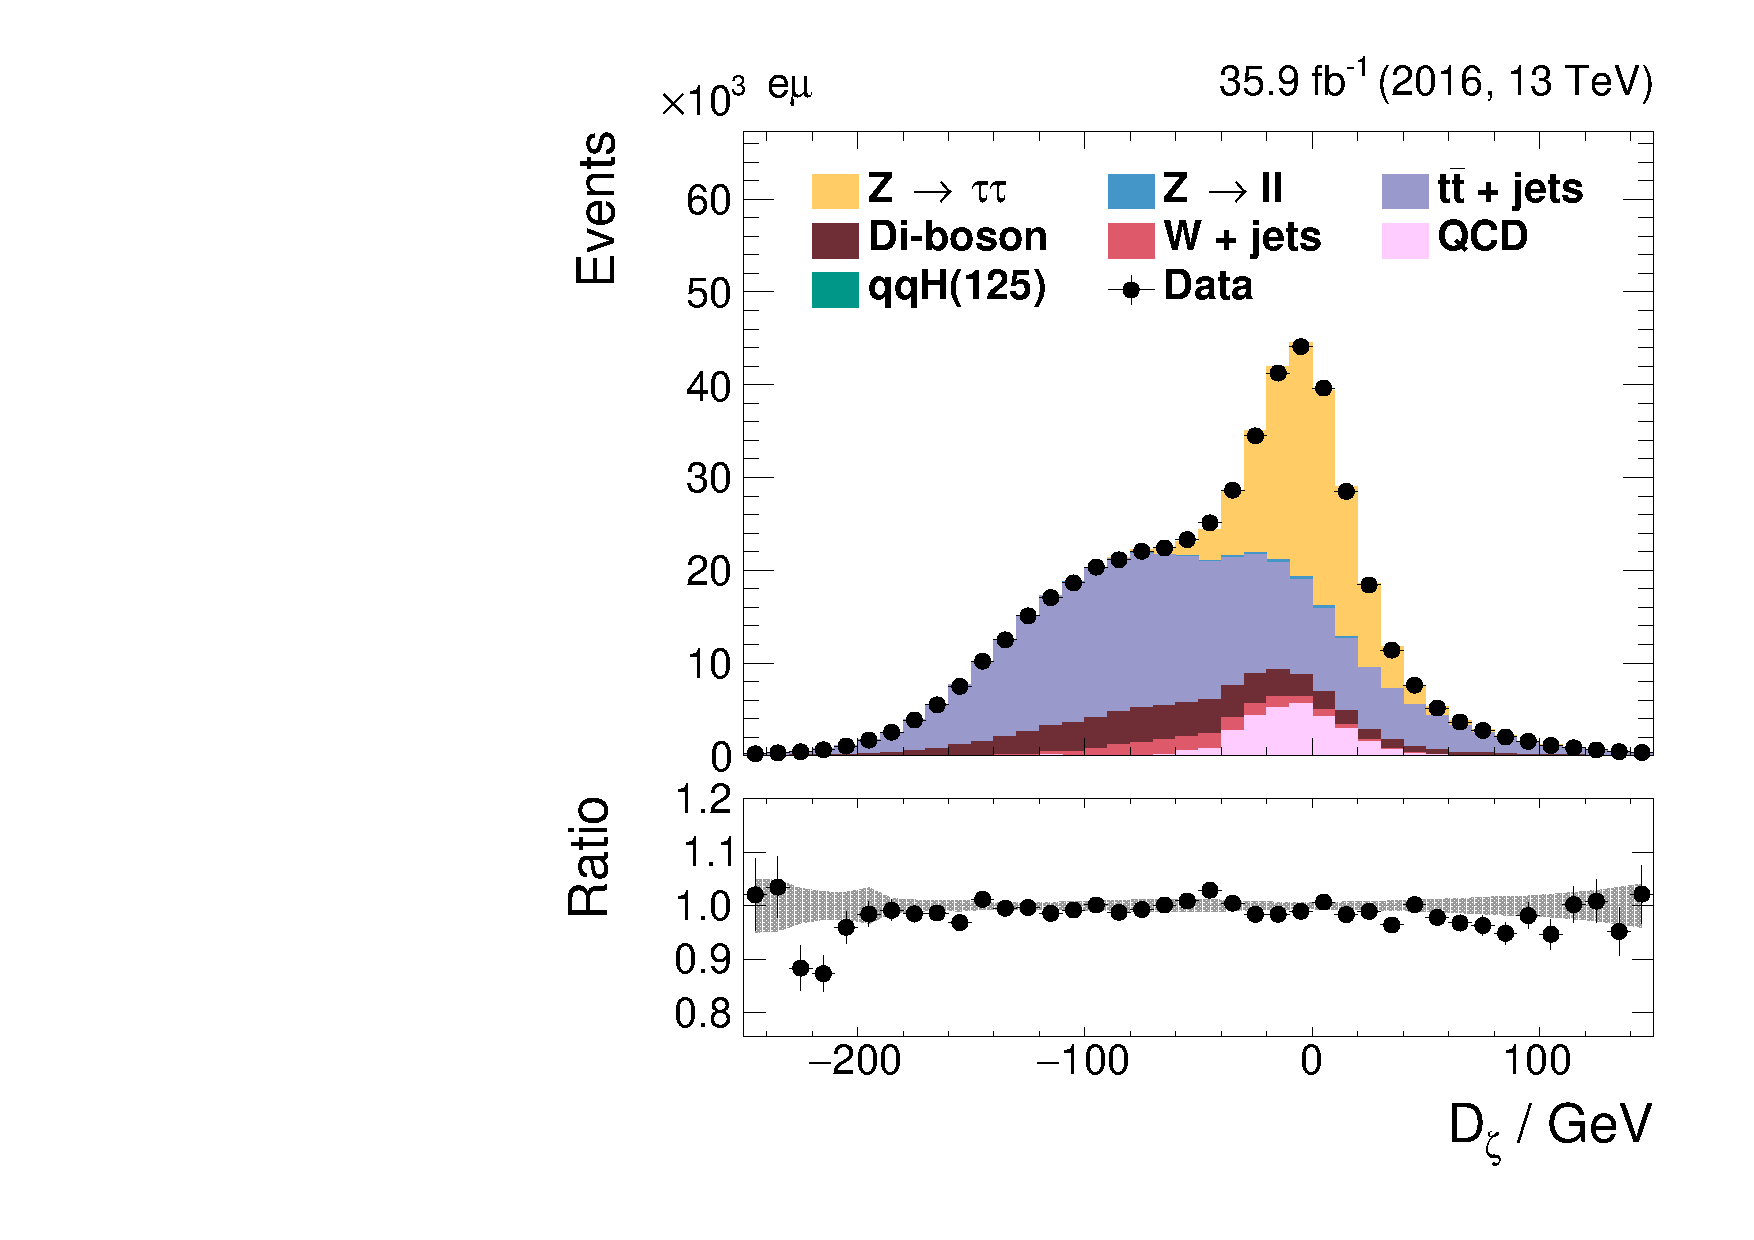
\includegraphics[width=0.47\textwidth]{Figures/eventselection/Categorization/em/pZetaMissVis.pdf}
    \caption[$D_{\zeta}$ inclusive distribution in the $e\mu$ channel.]{The inclusive background distribution and data of $D_{\zeta}$ neglecting the $m_\text{T}<\text{60\,{GeV}}$ baseline criterion and the b-tag veto for the $e\mu$ channel is shown. Requiring $D_{\zeta} < \text{-10\,{GeV}}$ the $t\bar{t}$ contribution is significantly reduced.}\label{dzeta}
\end{figure}%

\subsubsection{$t\bar{t}$ control region}

The initial normalization is derived taking into account the theory cross section, reconstruction and identification efficiencies, and the integrated luminosity. Later, a dedicated
$t\bar{t}$ control region is added to the final fit to adjust the $t\bar{t}$ normalization dynamically. The control region (CR) is 
constructed in the $e\mu$ channel by requiring 
\begin{equation}
    D_\zeta < \text{-50\,{GeV}} \text{\,and \,} m_\text{vis} > \text{90\,GeV} 
\end{equation}
and keeping all other selection criteria as defined in \textreft{sec:categorization} fixed.
The visible mass criterion is applied to reduce the small contamination of $\mathsf{Z\rightarrow\tau\tau}$ events leading to a purity of 82\% $t\bar{t}$ events in the control region.
The event content of the control region is shown in \figreft{bkg:ttbar:control_region}. 

% makePlots_controlPlots.py -i /nfs/dust/cms/user/dwolfsch/htautau/artus/2018-08-07_18-44_Run2CPStudies_Nominal_Summer16_plusHToTauTauM110-140/merged/ -s ztt zll ttj vv wj qcd ggh data -c em -x m_sv -e pzeta bveto -w "(pZetaMissVis<-50)*(m_vis>90)" --cpggh --background-method simeqn -a " --live --x-bins 1,0,250 --x-label \" m_{#tau#tau} / GeV\" --format png pdf " -r --www tt_controlregion --analysis-modules PrintInfos
\begin{figure}[h!]
    \centering
    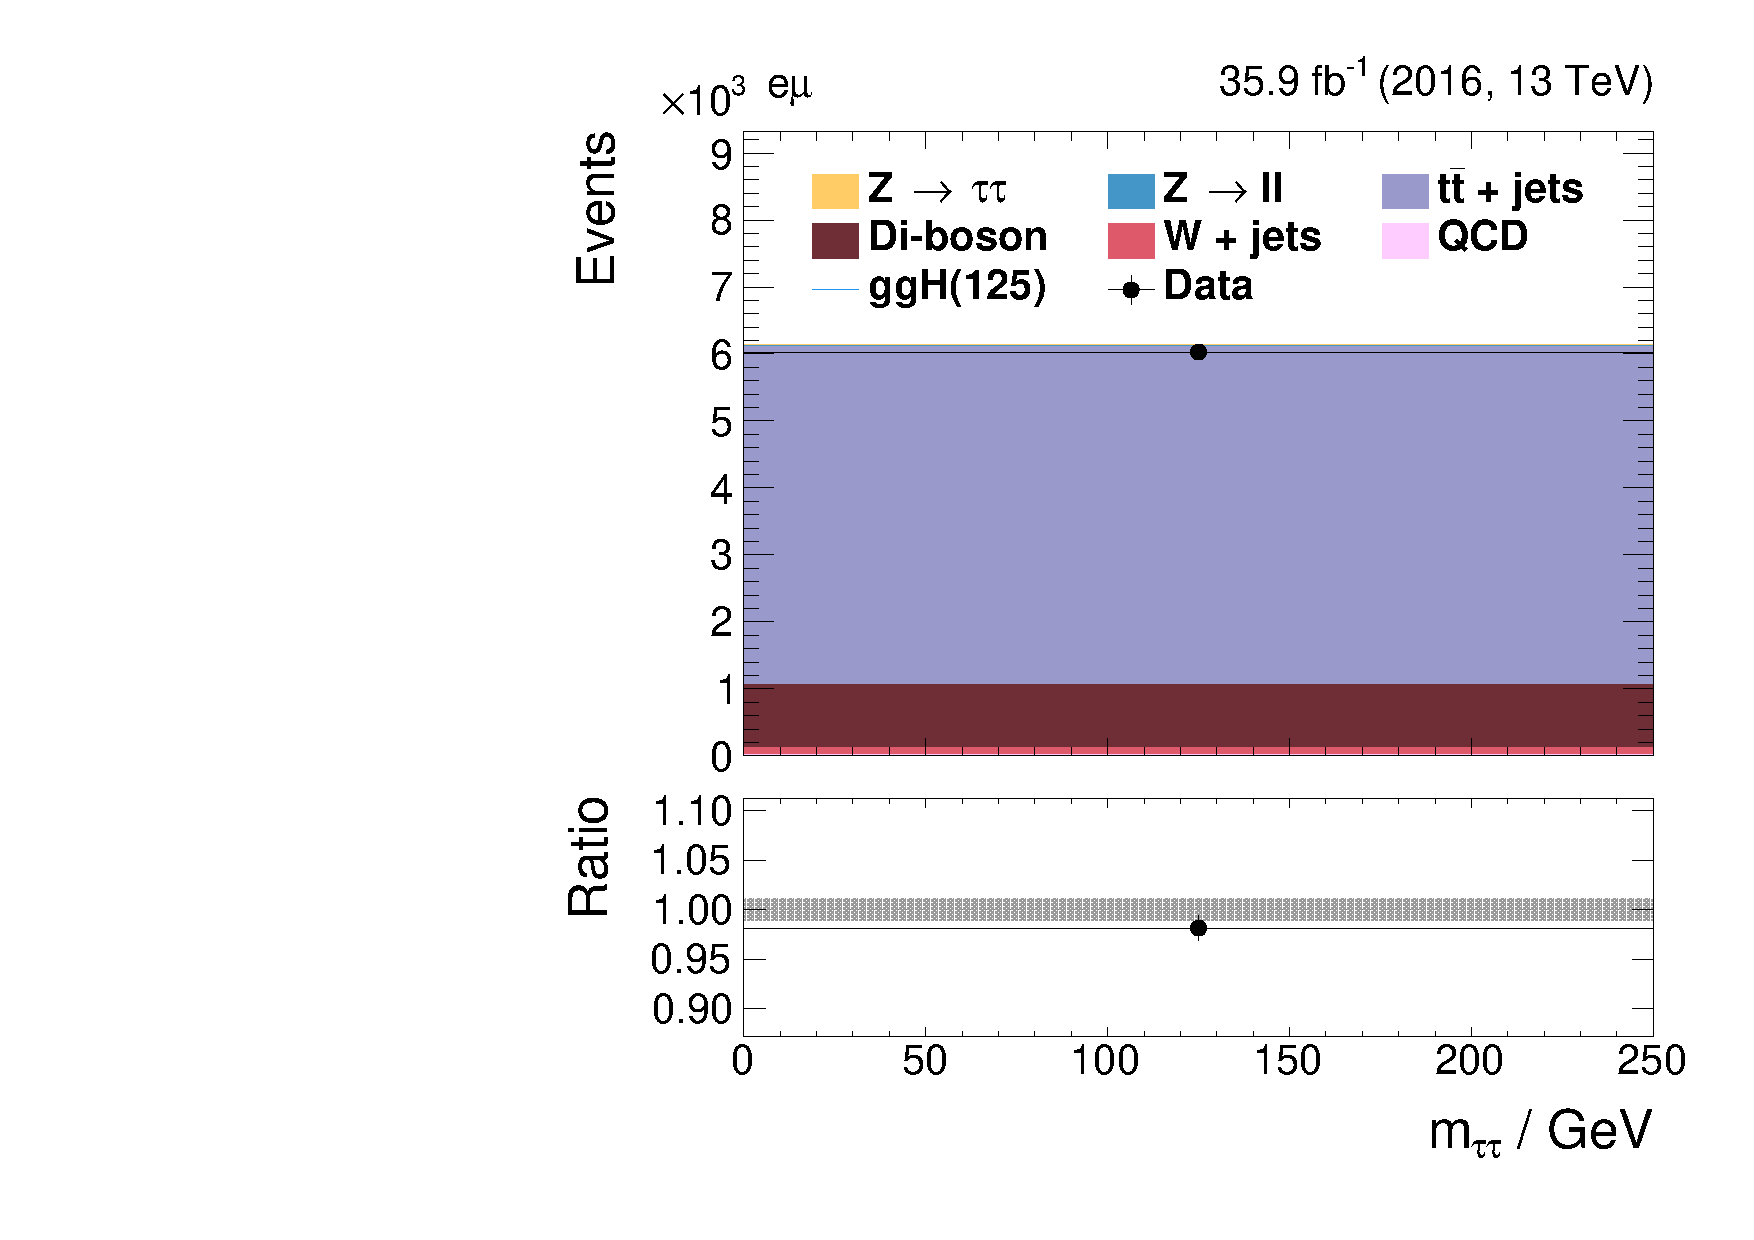
\includegraphics[width=.5\textwidth]{Figures/background_estimation/ttbar/m_sv.pdf}
    \caption[$t\bar{t}$ control region.]{Expected number of background events and data in the $t\bar{t}$ control region as given to the final fit.}\label{bkg:ttbar:control_region}
\end{figure}%

\subsection{W+jets}\label{sec:BackgroundEstimations:W}

\textit{W+jets} events are a major background of $\mathsf{H\rightarrow \tau\tau}$ events. Especially in the semileptonic channels \textit{W+jets} becomes large
if the W boson decays leptonically and one jet in the event is identified as a hadronically decaying tau lepton.
The estimation of \textit{W+jets} and \textit{QCD multijet} backgrounds distinguishes from the estimation of the other backgrounds as Monte Carlo 
generated events in that case do not provide a trustworthy prediction of the shape and yield of these backgrounds leading to large uncertainties.
Therefore, a new data-driven estimation technique is applied that provides 
a simultaneous estimation of both backgrounds in the semileptonic channels. 
Throughout this thesis \textit{QCD multijet background} is abbreviated by \textit{QCD}.  

\subsubsection{$e\mu$ and $\tau_\text{h}\tau_\text{h}$ channels}

In the $e\mu$ and $\tau_\text{h}\tau_\text{h}$ channels shape and yield are predicted from simulated \textit{W+jets} events.

\subsubsection{$e\tau_\text{h}$ and $\mu\tau_\text{h}$ channels}\label{sec:BackgroundEstimations:W:etmt}

\begin{figure}[h!]
    \centering
    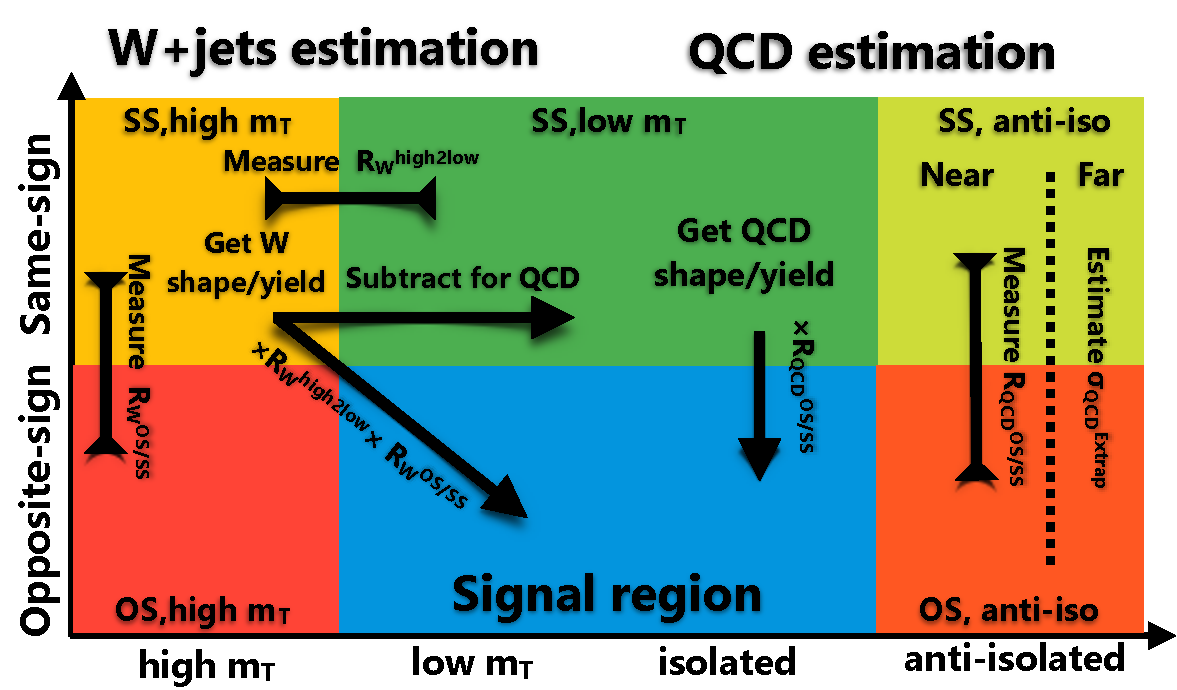
\includegraphics[width=.8\textwidth]{Figures/background_estimation/Wjets_etmt/Simeqn_method_2-crop.pdf}
    \caption[Simultaneous equation method.]{Procedure of the \textit{simultaneous equation method} - a data-driven estimation of \textit{W+jets} and \textit{QCD} backgrounds in the semileptonic ditau decay channels. 
    The shape and yield of the \textit{W+jets} background is taken from a \textit{W+jets} enriched sideband. This sideband is realized by selecting events with a transverse mass $m_\text{T}>\text{70\,GeV}$ ($\text{high } m_\text{T}$). 
    QCD is estimated from a sideband where the charged hadron and the lepton from the tau lepton decays have the same electric charge. Usually an estimate of \textit{W+jets} is needed to derive the QCD estimate in the sideband or vice-versa.
    Here, the $\text{high } m_\text{T}$ sideband is split again into same-sign and opposite-sign events (yellow and red boxes). By means of this, the \textit{W+jets} yield can be derived  
    in a same-sign control region and is calculated without a first estimate of the multijet contribution using formula \eqref{BR:eq:simeqn_1}. 
    For this, an opposite-sign to same-sign extrapolation factor $R_\text{W}^\text{OS/SS}$ must be measured (yellow and red boxes). Using further high-to-low (high2low) extrapolation factors (yellow and green boxes) the \textit{W+jets} yield can be estimated in every region. 
    As a consequence, the \textit{W+jets} contribution, that must be subtracted from data in a same-sign control region to get the shape and preliminary normalization for QCD events, is taken from the data-driven estimate in the yellow box.
    Last but not least, a QCD opposite-sign to same-sign extrapolation factor is measured in an additional sideband with inverted isolation of the light lepton (light-green and orange boxes).
    With all these factors the contribution of both \textit{W+jets} and \textit{QCD} can estimated in the signal region (blue box).}\label{BE:W:simeqn_method_sketch}
\end{figure}%

For the $e\tau_\text{h}$ and $\mu\tau_\text{h}$ channels the \textit{W+jets} contribution is determined using a high transverse mass control region (high $m_\text{T}$ CR) with $m_\text{T}>\text{70\,{GeV}}$. This CR is chosen because it profits from a high
purity of \textit{W+jets} events. %TODO: Whats the estimate for the purity?
In order to estimate the \textit{W+jets} background in this CR, all other sources of backgrounds are subtracted from data. Except for QCD, which is also estimated using a data-driven technique, all background shapes and 
yields are taken from simulation here. As a consequence, the estimation of \textit{W+jets} and \textit{QCD} backgrounds are entangled with each other and only the sum of both yields can be derived using a single CR. Splitting the high $m_\text{T}$ CR according to the electric charge the final state leptons possess
, the sum of yields of \textit{W+jets} and \textit{QCD} in both sub-CRs can be calculated. Thereby, \textit{SS} denotes events where the leptons have equal electric charges and \textit{OS} denotes events with oppositely charged leptons.
The yields in both subregions fulfill the following set of equations:
\begin{align}
    N_\text{W}^\text{SS,CR} + N_\text{QCD}^\text{SS,CR} &= N_\text{data}^\text{SS,CR} - N_\text{other}^\text{SS,CR} \\
    N_\text{W}^\text{OS,CR} + N_\text{QCD}^\text{OS,CR} &= N_\text{data}^\text{OS,CR} - N_\text{other}^\text{OS,CR}. 
\end{align}
Solving them for $N_\text{W}^\text{SS,CR}$, the \textit{W+jets} yield in the SS high $m_\text{T}$ region can be determined without a first estimate 
of the \textit{QCD} background.
First, the OS yields of \textit{QCD} and \textit{W+jets} is expressed by the OS/SS extrapolation factors $R_\text{QCD}^\text{OS/SS}$ and  $R_\text{W}^\text{OS/SS}$:
\begin{align*}
    \begin{cases}  
        N_\text{QCD}^\text{SS,CR} &= N_\text{data}^\text{SS,CR} - N_\text{other}^\text{SS,CR} - N_\text{W}^\text{SS,CR} \\
        R_\text{W}^\text{OS/SS} \cdot N_\text{W}^\text{SS,CR} &= N_\text{data}^\text{OS,CR} - N_\text{other}^\text{OS,CR} - R_{QCD}^{OS/SS}\cdot N_{QCD}^{SS,CR} 
    \end{cases}
\end{align*}
$N_\text{QCD}^\text{SS,CR}$ can then by substituted by the upper equation
\begin{align*}
    &\Rightarrow R_\text{W}^\text{OS/SS} \cdot N_\text{W}^\text{SS,CR} = N_\text{data}^\text{OS,CR} - N_\text{other}^\text{OS,CR} - R_\text{QCD}^\text{OS/SS}\cdot \left( N_\text{data}^\text{SS,CR} - N_\text{other}^\text{SS,CR} - N_\text{W}^\text{SS,CR} \right).   
\end{align*}
After that $N_\text{W}^\text{SS,CR}$ is extracted
\begin{align*}
    &\Rightarrow R_\text{W}^\text{OS/SS} \cdot N_\text{W}^\text{SS,CR} - R_\text{QCD}^\text{OS/SS} N_\text{W}^\text{SS,CR}  = N_\text{data}^\text{OS,CR} - N_\text{other}^\text{OS,CR} - R_\text{QCD}^\text{OS/SS}\cdot \left( N_\text{data}^\text{SS,CR} - N_\text{other}^\text{SS,CR} \right)    
\end{align*} 
giving an expression that is independent of the \textit{QCD} yield in the high $m_\text{T}$ SS region:
\begin{align}\label{BR:eq:simeqn_1}
\Rightarrow N_\text{W}^\text{SS,CR} &=  \frac{1}{R_\text{W}^\text{OS/SS}-R_\text{QCD}^\text{OS/SS}} \left(  N_\text{data}^\text{OS,CR} - N_\text{other}^\text{OS,CR} - R_\text{QCD}^\text{OS/SS}\cdot \left( N_\text{data}^\text{SS,CR} - N_\text{other}^\text{SS,CR} \right) \right).
\end{align}
This approach is called \textit{simultaneous equation method} and its major advantage compared to the approach used in \cite{Sirunyan:2017khh} is that no
\textit{W+jets} Monte Carlo is needed to calculate the yield of \textit{QCD} in the control region to later determine the shape and yield of \textit{W+jets} there. 
This implies that the yield of \textit{W+jets} is obtained naturally by this technique and no \textit{QCD} Monte Carlo sample is needed at all. 
The technique is visualized in the sketch in \figreft{BE:W:simeqn_method_sketch}.

The \textit{W+jets} yield in the signal region is finally extrapolated utilizing
\begin{equation}
    N_\text{W}^\text{SR} = R_\text{W}^\text{SS,high2low}\cdot R_\text{W}^\text{OS/SS}\cdot N_\text{W}^\text{SS,CR}. 
\end{equation}\label{BR:eq:simeqn_2}
Summarizing the procedure above, three extrapolation factors need to be measured: %An additional third factor is needed to estimate the same-sign \textit{QCD} yield.
\begin{enumerate}
    \item A \textit{W+jets} OS/SS extrapolation factor $R_\text{W}^\text{OS/SS}$ that is measured using simulated \textit{W+jets} events. For the \textit{0-jet} and \textit{boosted} categories, this factor is measured in events that satisfy the criterion $m_\text{T}>\text{70\,{GeV}}$. For the two dijet categories, an inclusive selection is utilized by omitting the requirement that events must have a transverse mass smaller than $\text{50\,GeV}$.
    \item A \textit{QCD} OS/SS extrapolation factor $R_\text{QCD}^\text{OS/SS}$ that is measured from data in a sideband with anti-isolated leptons (see section \ref{sec:qcdosss} and the light-green and orange sideband in \figreft{BE:W:simeqn_method_sketch}).
    \item A \textit{W+jets} high transverse mass ($m_\text{T}>\text{70\,{GeV}}$) to low transverse mass ($m_\text{T}<\text{50\,{GeV}}$) extrapolation factor $R_\text{W}^\text{OS/SS,high2low}$ that is measured using Monte Carlo simulated \textit{W+jets} events and is calculated in SS and OS events, respectively.
\end{enumerate} 

In the following subsections the results for the measurement of the different \textit{W+jets} extrapolation factors are discussed. 
The procedure of measuring the \textit{QCD} OS/SS factor is described in section \ref{sec:qcdosss}. 

\paragraph{W+jets extrapolation factors}\mbox{}\\
Simulated \textit{W+jets} events are utilized to measure all three \textit{W+jets} extrapolation factors. 
Figure \ref{W:Scale_factors} (left) shows the measured OS/SS factors in each category for both channels. Only statistical uncertainties are shown here.
The OS/SS ratios for both $m_\text{T}$ control regions were found to not always agree within their uncertainties. 
Therefore, it was decided that $R_\text{W}^\text{OS/SS}$ cannot be measured in an inclusive $m_\text{T}$ distribution for all categories
and the high $m_\text{T}$ control region is used to measure the factor only in the \textit{0-jet} and the \textit{boosted} categories.
In the dijet categories the statistics become so low that the factors agree within their uncertainties and $R_\text{W}^\text{OS/SS}$ can be measured without distinguishing between different transverse mass regions. As a consequence, factors measured in the inclusive selection profit from a larger bin population. 
The trend clearly indicates, that the OS/SS factor depend on the number of jets in the events implying that the \textit{W+jets} extrapolation factors must be measured for each signal category individually.
The high-to-low transverse mass extrapolation factors are measured individually for OS and SS events, because they should be as proximate as possible to the region where they are applied,  and are shown in figure \ref{W:Scale_factors} in the right canvas.
The exact scale factors with their associated statistical uncertainties of the measurements for both $e\tau_\text{h}$ and $\mu\tau_\text{h}$ channels for all 
signal categories are summarized in tables \ref{tab:etmt_wj:wj_factors_0jet1jet} and \ref{tab:etmt_wj:wj_factors_2jet}, respectively.

\begin{table}[h!]
    \centering
    \caption[Measured W+jets extrapolation factors and associated statistical uncertainties in the \textit{0-jet} and \textit{boosted} categories.]{Measured W+jets extrapolation factors and associated statistical uncertainties in the \textit{0-jet} and \textit{boosted} categories. $R_\text{W}^\text{OS/SS}$ is measured in the high $m_\text{T}$ region for these two categories. The relative uncertainty of the measurement is given in the brackets.}\label{tab:etmt_wj:wj_factors_0jet1jet}
    \begin{tabular}{lclll}
        \toprule
         Category              & Channel    & $R_\text{W}^{\text{OS/SS, }m_\text{T}>\text{70\,GeV}}$         & $R_\text{W}^\text{SS,high2low}$ & $R_\text{W}^\text{OS,high2low}$\\ \hline
        \multirow{2}{*}{0-jet} & $e\tau_\text{h}$   & {\footnotesize $\text{5.14} \pm \text{0.08 (1.4\%)}$ }& {\footnotesize $\text{0.284} \pm \text{0.003 (1.3\%)}$ }       & {\footnotesize $\text{0.283} \pm \text{0.008 (2.8\%)}$ }      \\
                               & $\mu\tau_\text{h}$ & {\footnotesize $\text{5.39} \pm \text{0.06 (1.0\%)}$ }& {\footnotesize $\text{0.301} \pm \text{0.003 (0.9\%)}$ }       & {\footnotesize $\text{0.300} \pm \text{0.006 (2.0\%)}$ }      \\
        \multirow{2}{*}{boosted}& $e\tau_\text{h}$   &{\footnotesize  $\text{3.84} \pm \text{0.07 (1.8\%)}$} &{\footnotesize  $\text{0.282} \pm \text{0.005 (1.8\%)}$}        &{\footnotesize  $\text{0.269} \pm \text{0.010 (3.6\%)}$}       \\
                               & $\mu\tau_\text{h}$ & {\footnotesize $\text{3.39} \pm \text{0.04 (1.2\%)}$ }& {\footnotesize $\text{0.295} \pm \text{0.003 (1.3\%)}$ }       & {\footnotesize $\text{0.313} \pm \text{0.007 (2.2\%)}$ }      \\
    \end{tabular}% 
\end{table}%     
\begin{table}[h!]
    \centering
    \caption[Measured W+jets extrapolation factors and associated statistical uncertainties in the \textit{dijet lowboost} and \textit{dijet boosted} categories.]{Measured W+jets extrapolation factors and associated statistical uncertainties in the \textit{dijet lowboost} and \textit{dijet boosted} categories. The full region of $m_\text{T}$ events, omitting the baseline $m_\text{T}<\text{50\,GeV}$ criterion, is taken to measure $R_\text{W}^\text{OS/SS}$.
    Relative uncertainties of the measurement are stated in the brackets.}\label{tab:etmt_wj:wj_factors_2jet}
    \begin{tabular}{lclll}
        \toprule
         Category                       & Channel    & $R_\text{W}^\text{OS/SS}$          & $R_\text{W}^\text{OS,high2low}$ & $R_\text{W}^\text{SS,high2low}$   \\ \hline
        \multirow{2}{*}{2-jet lowboost} & $e\tau_\text{h}$   & {\footnotesize $\text{2.70} \pm \text{0.20 (7.6\%)}$}  &  {\footnotesize $\text{0.291} \pm \text{0.024 (8.2\%)}$ }       &{\footnotesize $\text{0.185} \pm \text{0.024 (13.2\%)}$}    \\
                                        & $\mu\tau_\text{h}$ & {\footnotesize $\text{2.70} \pm \text{0.15 (5.4\%)}$}  &  {\footnotesize $\text{0.300} \pm \text{0.017 (5.9\%)}$ }      & {\footnotesize $\text{0.209} \pm \text{0.018 (8.8\%)}$ }          \\
        \multirow{2}{*}{2-jet boosted}  & $e\tau_\text{h}$   & {\footnotesize $\text{2.96} \pm \text{0.73 (25\%)}$ }  &  {\footnotesize $\text{0.376} \pm \text{0.089 (23\%)}$  }      & {\footnotesize $\text{0.249} \pm \text{0.098 (39\%)}$  } \\
                                        & $\mu\tau_\text{h}$ & {\footnotesize $\text{2.59} \pm \text{0.50 (19\%)}$ }  &  {\footnotesize $\text{0.463} \pm \text{0.084 (18\%)}$  }      & {\footnotesize $\text{0.250} \pm \text{0.068 (28\%)}$  } \\
    \end{tabular}%
\end{table}%

% higgsplot.py -j osss_sf_Wjets.json
% higgsplot.py -j h2l_Wjets.json
\begin{figure}[h!]
    \centering
    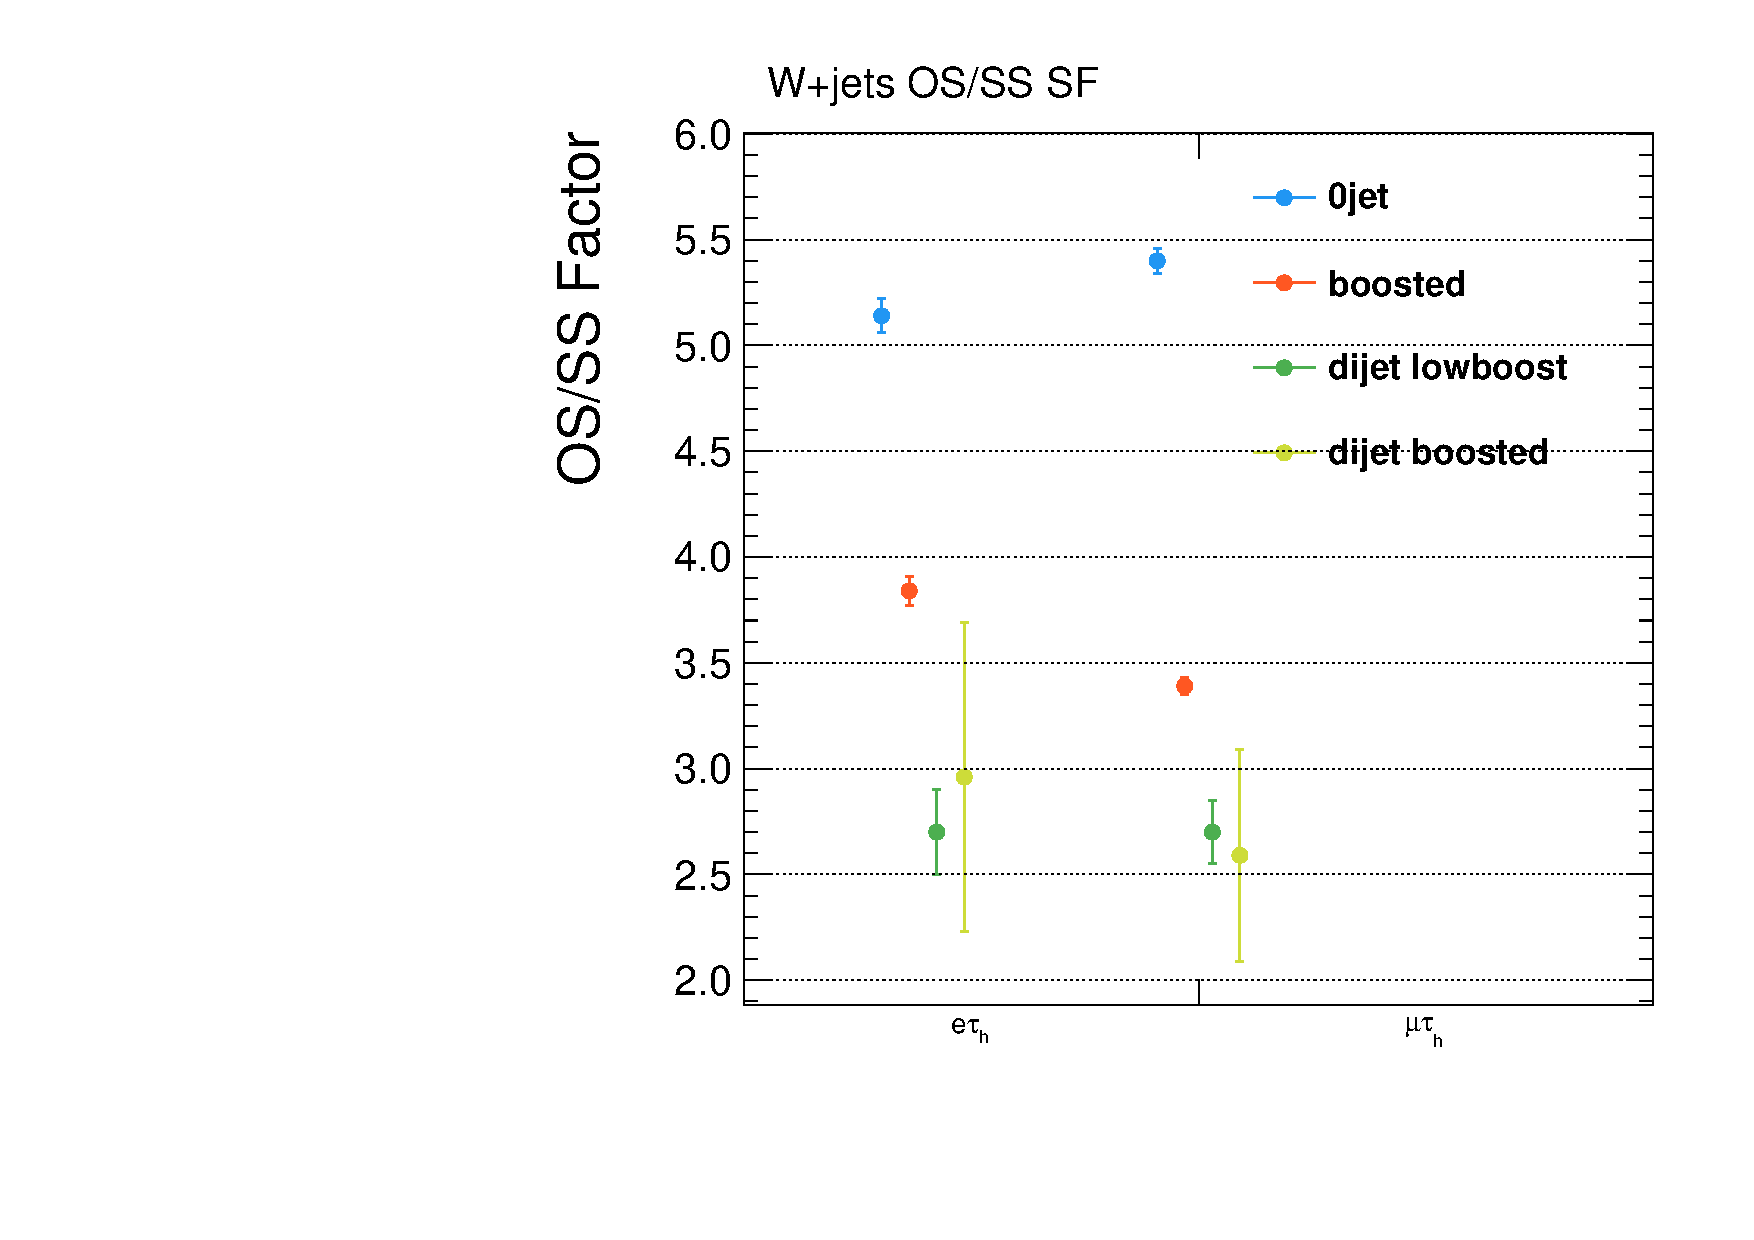
\includegraphics[width=0.47\textwidth]{Figures/background_estimation/Wjets_OSSS.pdf}
    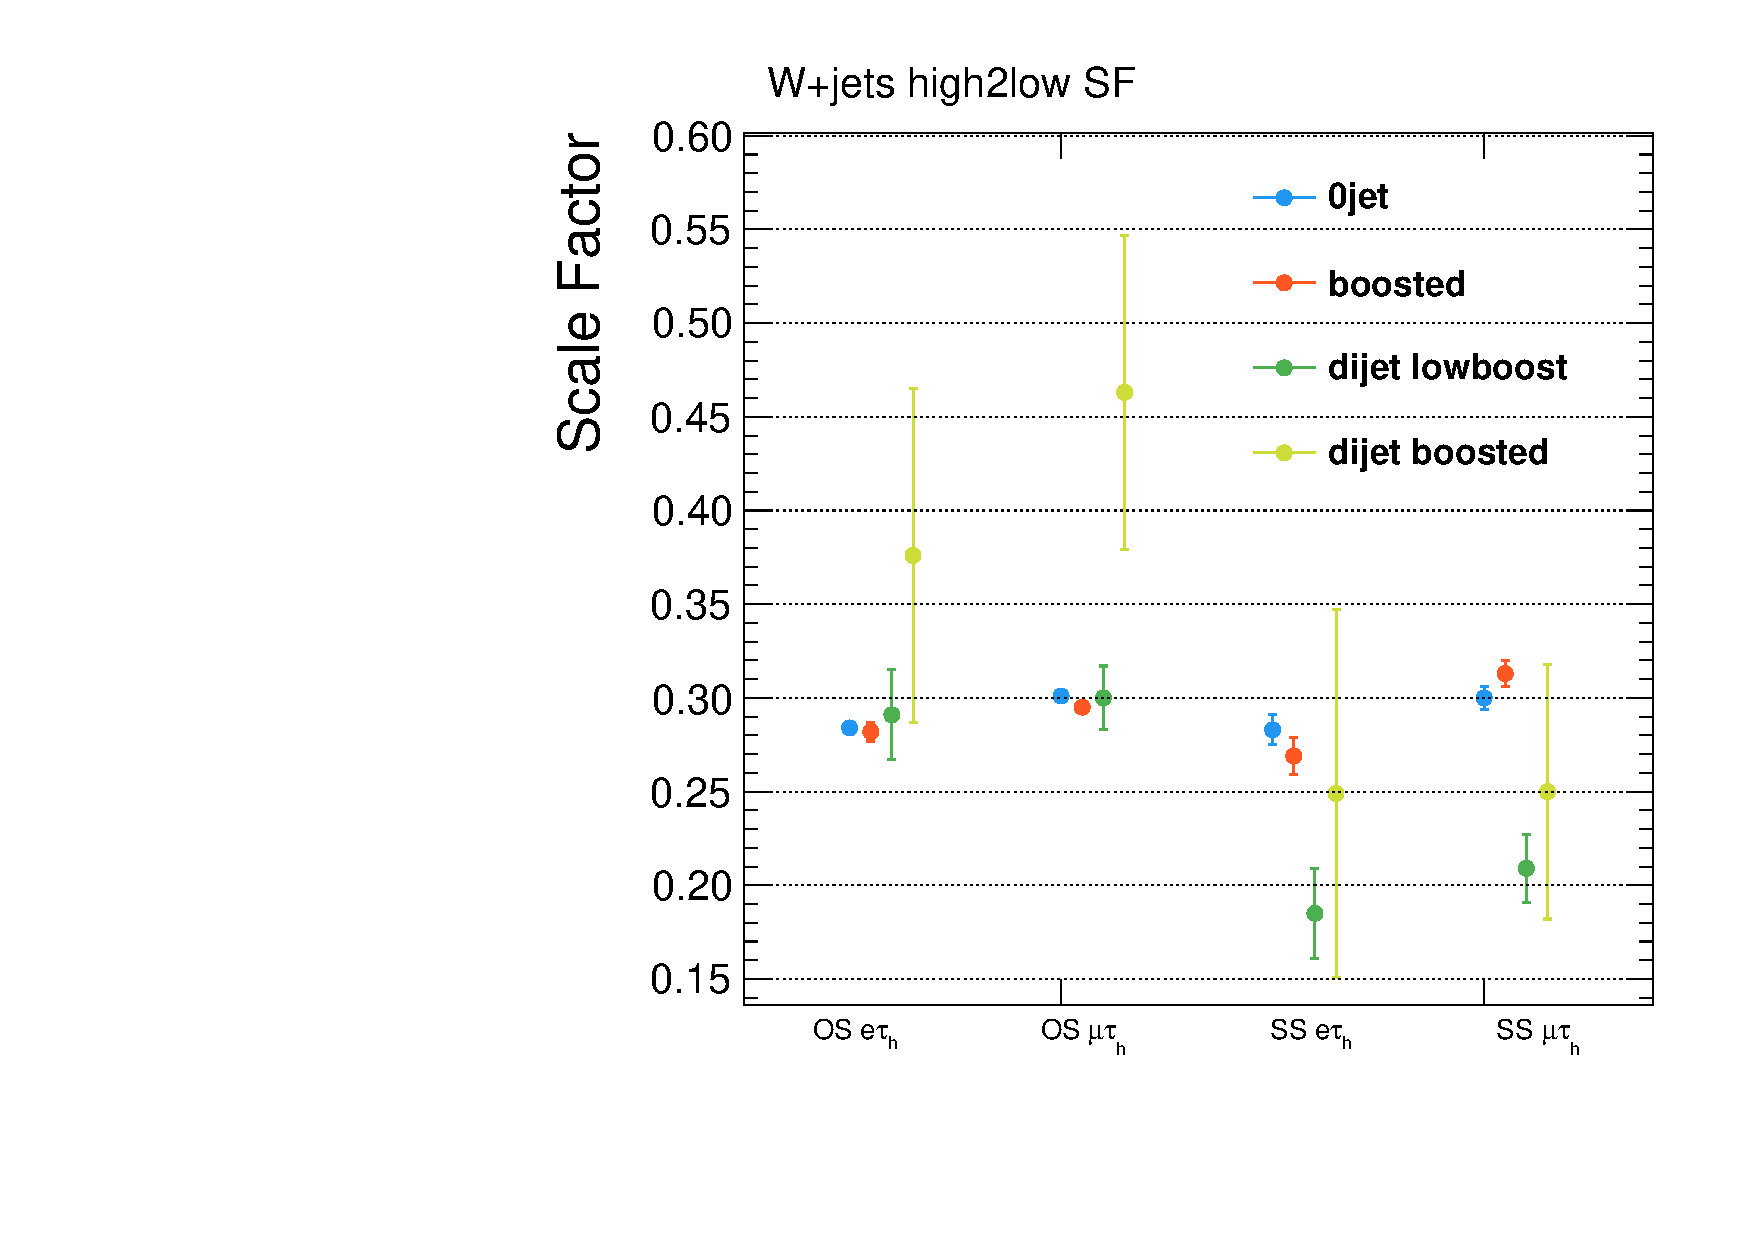
\includegraphics[width=0.47\textwidth]{Figures/background_estimation/Wjets_h2l.pdf}
    \caption[\textit{W+jets} extrapolation factors.]{\textit{W+jets} OS/SS extrapolation factors (left) and high $m_\text{T}$ to low $m_\text{T}$ scale factors (right) measured from simulated events.
    For the OS/SS factors a clear dependence on the number of jets is noted as the factors strongly depend on the number of jets of the different categories.}\label{W:Scale_factors}
\end{figure}

\paragraph{W+jets systematic uncertainties}\mbox{}\\
Systematic uncertainties covering the extrapolation from the high $m_\text{T}$ CR to the signal region are calculated using the Ersatz method \cite{higMSSM}.
In addition to the high $m_\text{T}$ to low $m_\text{T}$ uncertainty, there is a low $p_{\,\text{T}}$ to high $p_{\,\text{T}}$ extrapolation uncertainty 
in the \textit{dijet boosted} category that takes the higher Higgs boson transverse momentum regime in this region into account.\newline{}
As the \textit{W+jets} OS/SS factor is estimated from simulated events a potential mismodeling of these events is accounted for by systematic uncertainties on the 
this factor. These uncertainties are estimated in a CR with inverted isolation of the hadronically decaying tau lepton. Other background contributions are subtracted from data in this sideband separately for OS and SS events. The OS/SS factor is measured from this data-driven \textit{W+jets} estimate and then compared
to the MC estimate from before. The difference $\abs{R_\text{W}^\text{OS/SS, data}-R_\text{W}^\text{OS/SS, MC}}$ is used as systematic uncertainty and is measured in the \textit{0-jet}, \textit{boosted} and an inclusive \textit{dijet} category. These uncertainties were measured in \cite{danny2} and are summarized in \tabreft{BR:W:ersatz}. 
For the dijet categories a single uncertainty was measured. 
\begin{table}
    \centering
    \caption[List of \textit{W+jets} systematic uncertainties arising from the background estimation.]{Systematic uncertainties arising from the \textit{W+jets} background estimation method. Extrapolation uncertainties are derived using the \textit{Ersatz method} from \cite{higMSSM} in the \textit{0-jet} and \textit{boosted} categories. Uncertainties for the \textit{dijet lowboost} and \textit{dijet boosted} categories are 
    measured in an inclusive selection for both categories simultaneously. An additional low $p_{\,\text{T}}$ to high $p_{\,\text{T}}$ extrapolation uncertainty is used in the \textit{dijet boosted} category.
    \textit{W+jets} OS/SS uncertainties were measured by comparing simulated events with data in a sideband with a relaxed selection of hadronically decaying tau leptons.
    As these uncertainties affect only the rate of the \textit{W+jets} process, they are assigned as log-normal (lnN) uncertainties.}\label{BR:W:ersatz}
    \begin{tabular}{llll}
        \toprule
        Name & Channel & Type & Value \\ \midrule
        \multicolumn{4}{c}{Ersatz method} \\ \midrule
        WHighMTtoLowMT\_0jet\_CHANNEL\_13TeV & $e\tau_\text{h}$, $\mu\tau_\text{h}$ & lnN &     3.3\%           \\    
        WHighMTtoLowMT\_boosted\_CHANNEL\_13TeV & $e\tau_\text{h}$, $\mu\tau_\text{h}$ & lnN &   6.7\%          \\    
        WHighMTtoLowMT\_dijet\_CHANNEL\_13TeV & $e\tau_\text{h}$, $\mu\tau_\text{h}$ & lnN &  18.2\%     \\    
        WlowPTtoHighPT\_dijet\_boosted\_CHANNEL\_13TeV & $e\tau_\text{h}$, $\mu\tau_\text{h}$ & lnN &  27.9\%     \\    \midrule
        \multicolumn{4}{c}{Data-MC comparison} \\ \midrule
        WOSSS\_syst\_0jet\_et\_13TeV & $e\tau_\text{h}$ & lnN &  0.2\%     \\   
        WOSSS\_syst\_boosted\_et\_13TeV & $e\tau_\text{h}$ & lnN &  2.9\%     \\   
        WOSSS\_syst\_dijet\_et\_13TeV & $e\tau_\text{h}$ & lnN &  13.1\%     \\
        WOSSS\_syst\_0jet\_mt\_13TeV & $\mu\tau_\text{h}$ & lnN &  1.2\%     \\   
        WOSSS\_syst\_boosted\_mt\_13TeV & $\mu\tau_\text{h}$ & lnN &  4.9\%     \\   
        WOSSS\_syst\_dijet\_mt\_13TeV & $\mu\tau_\text{h}$ & lnN &  8.6\%     \\   
        WOSSS\_stat\_0jet\_et\_13TeV & $e\tau_\text{h}$ & lnN &  3.5\%     \\   
        WOSSS\_stat\_boosted\_et\_13TeV & $e\tau_\text{h}$ & lnN &  2.6\%     \\   
        WOSSS\_stat\_dijet\_et\_13TeV & $e\tau_\text{h}$ & lnN &  8.2\%     \\
        WOSSS\_stat\_0jet\_mt\_13TeV & $\mu\tau_\text{h}$ & lnN &  2.6\%     \\   
        WOSSS\_stat\_boosted\_mt\_13TeV & $\mu\tau_\text{h}$ & lnN &  2.0\%     \\   
        WOSSS\_stat\_dijet\_mt\_13TeV & $\mu\tau_\text{h}$ & lnN &  6.6\%     \\  \bottomrule  
    \end{tabular}
\end{table}
 
\paragraph{Control plots}\mbox{} \\
The results of the background estimation for the transverse mass variable are shown for all categories in figures \ref{fig:etmt_wj:wj_control_0jet}-\ref{fig:etmt_wj:wj_control_boosted}. The distribution of data are blinded in the signal region up 
to $m_\text{T}<\text{50\,GeV}$ and only statistical uncertainties are taken into account. 
After the background estimation, an overall good agreement between data and simulation in the high $m_\text{T}$ region is observed.

% python HiggsAnalysis/KITHiggsToTauTau/scripts/makePlots_controlPlots.py -i /nfs/dust/cms/user/dwolfsch/htautau/artus/2018-08-07_18-44_Run2CPStudies_Nominal_Summer16_plusHToTauTauM110-140/merged/ -s ztt zll ttj vv wj qcd qqh gghjhusm data -c et mt -x mt_1 --categories ZeroJetCP BoostedCP dijet2D_lowboost dijet2D_boosted -a "   --live --mask-histogram-nicks data ratio_Data --mask-below-threshold 50  --formats png pdf --y-subplot-lims 0.7 1.3 " --background-method simeqn --cpggh --www BackgroundEstimation/control_plots/ -r --analysis-modules MaskHistograms -n 8  
\begin{figure}[h!]
 \centering
  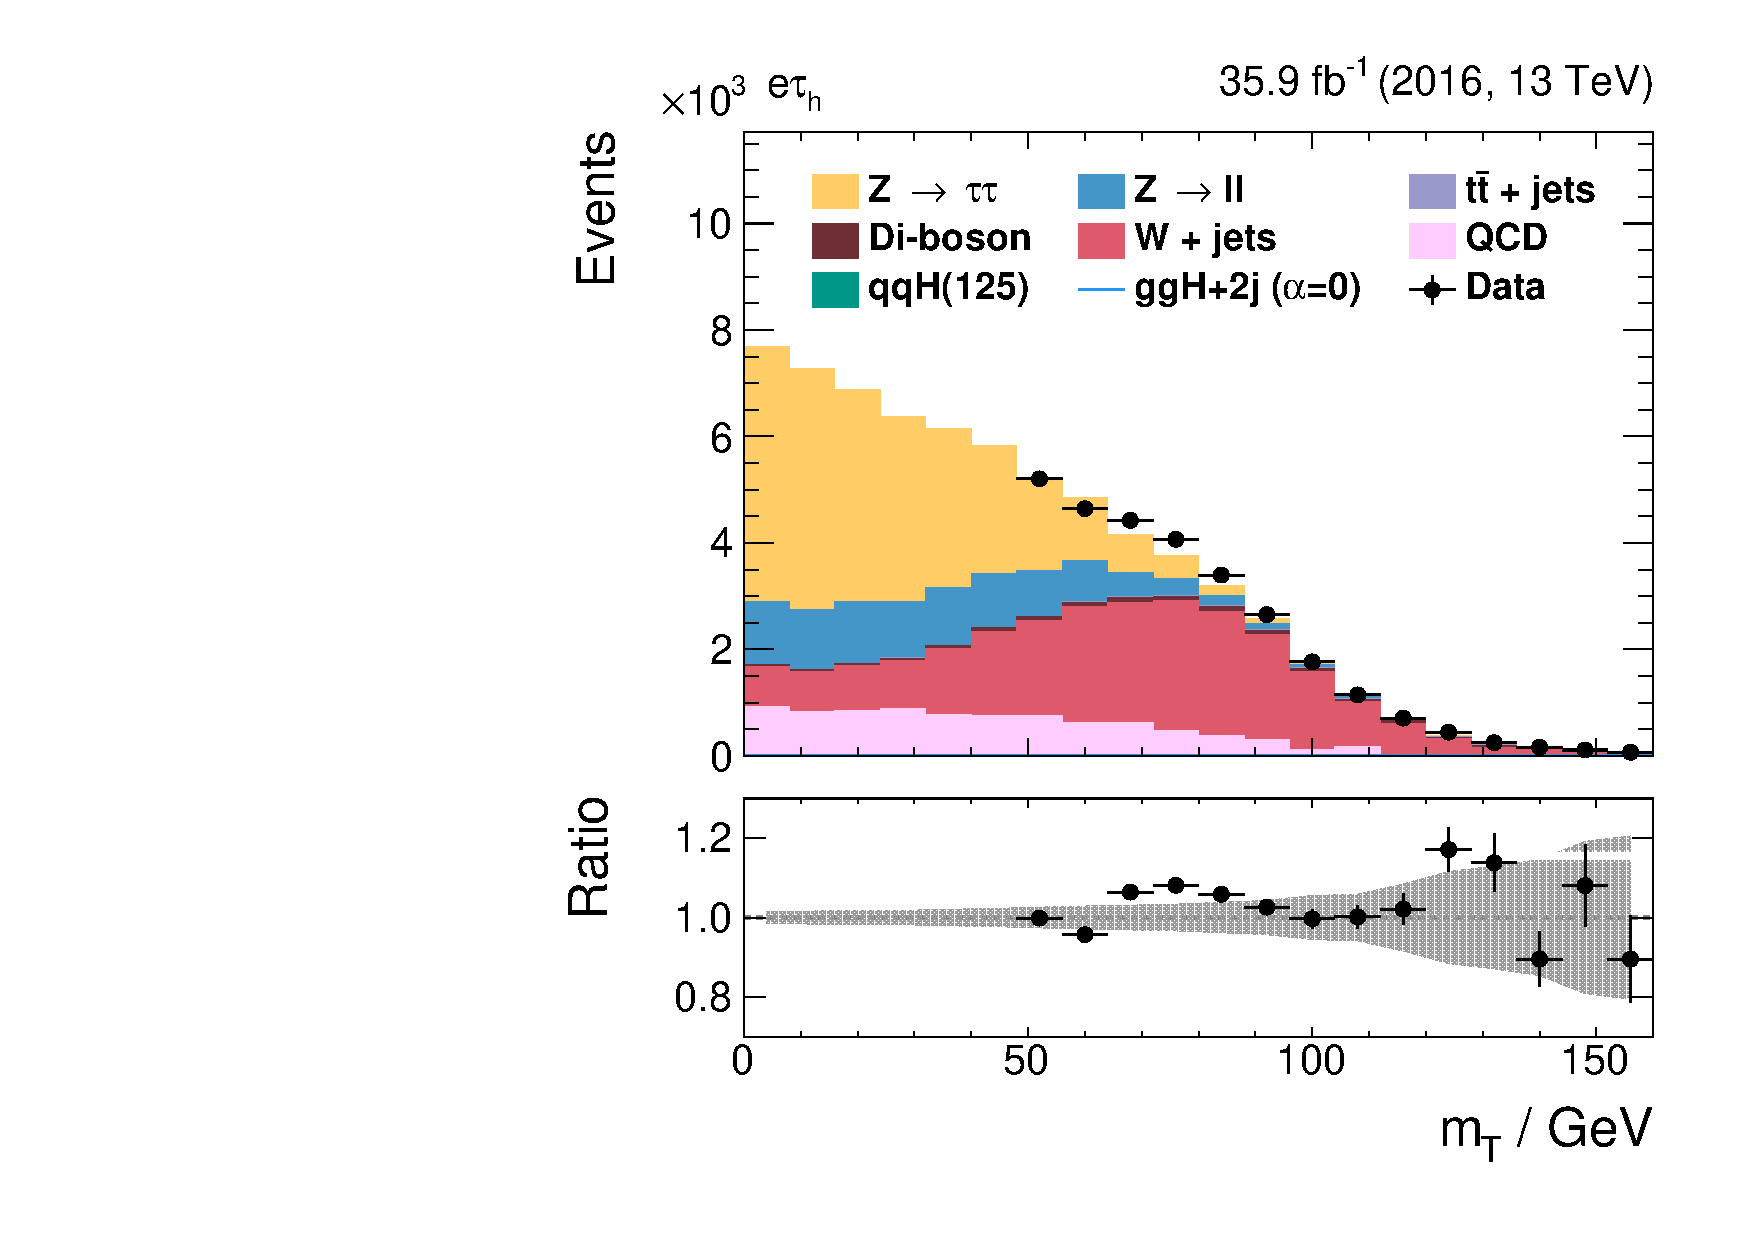
\includegraphics[width=0.47\textwidth]{Figures/background_estimation/control_plots/et/ZeroJetCP/mt_1.pdf}
  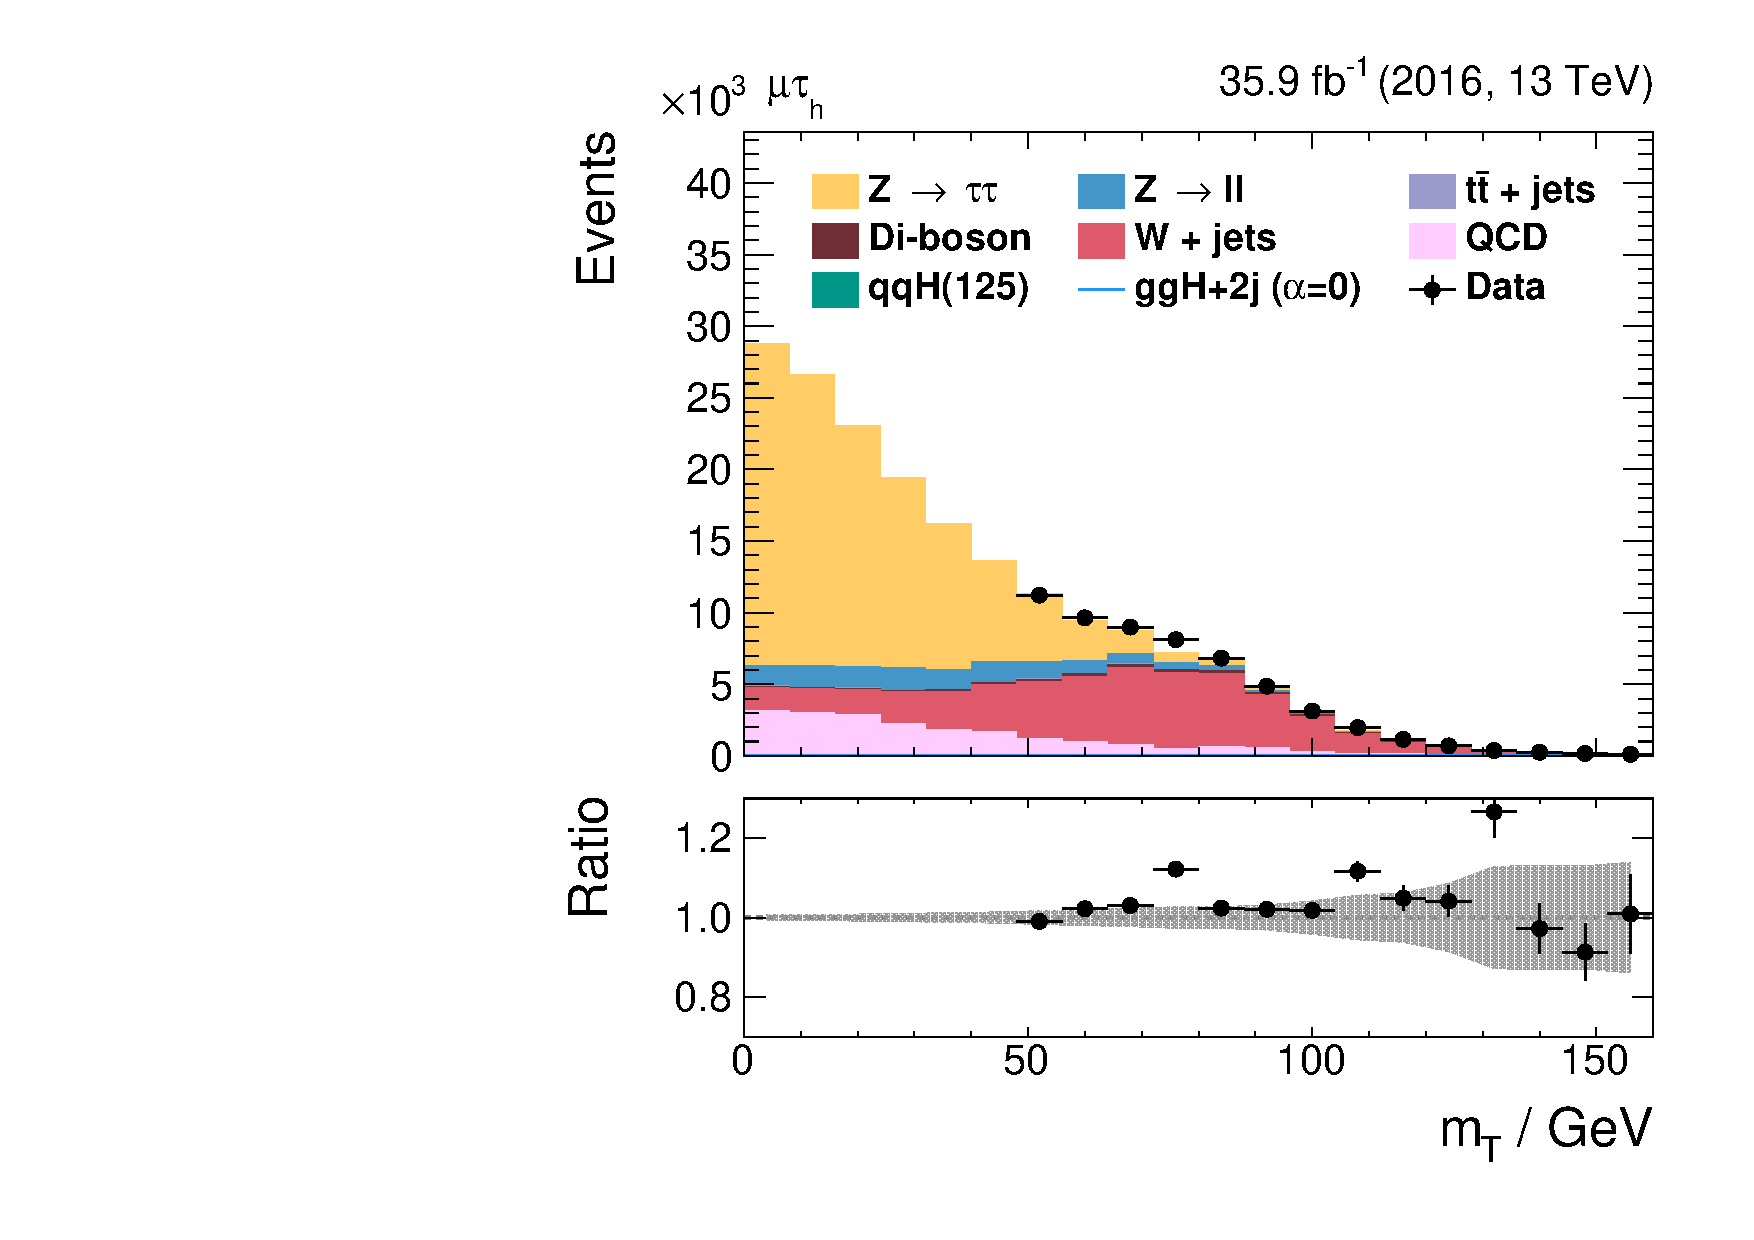
\includegraphics[width=0.47\textwidth]{Figures/background_estimation/control_plots/mt/ZeroJetCP/mt_1.pdf}  
\caption[\textit{W+jets} control plots in the \textit{0-jet} category.]{Blinded $m_\text{T}$ distribution in the \textit{0-jet} category for the $e\tau_\text{h}$ (left) and $\mu\tau_\text{h}$ (right) channel.
Backgrounds were estimated with the techniques introduced in section \ref{sec:background_estimation}.}\label{fig:etmt_wj:wj_control_0jet}
\end{figure}  
\begin{figure}[h!]
 \centering
  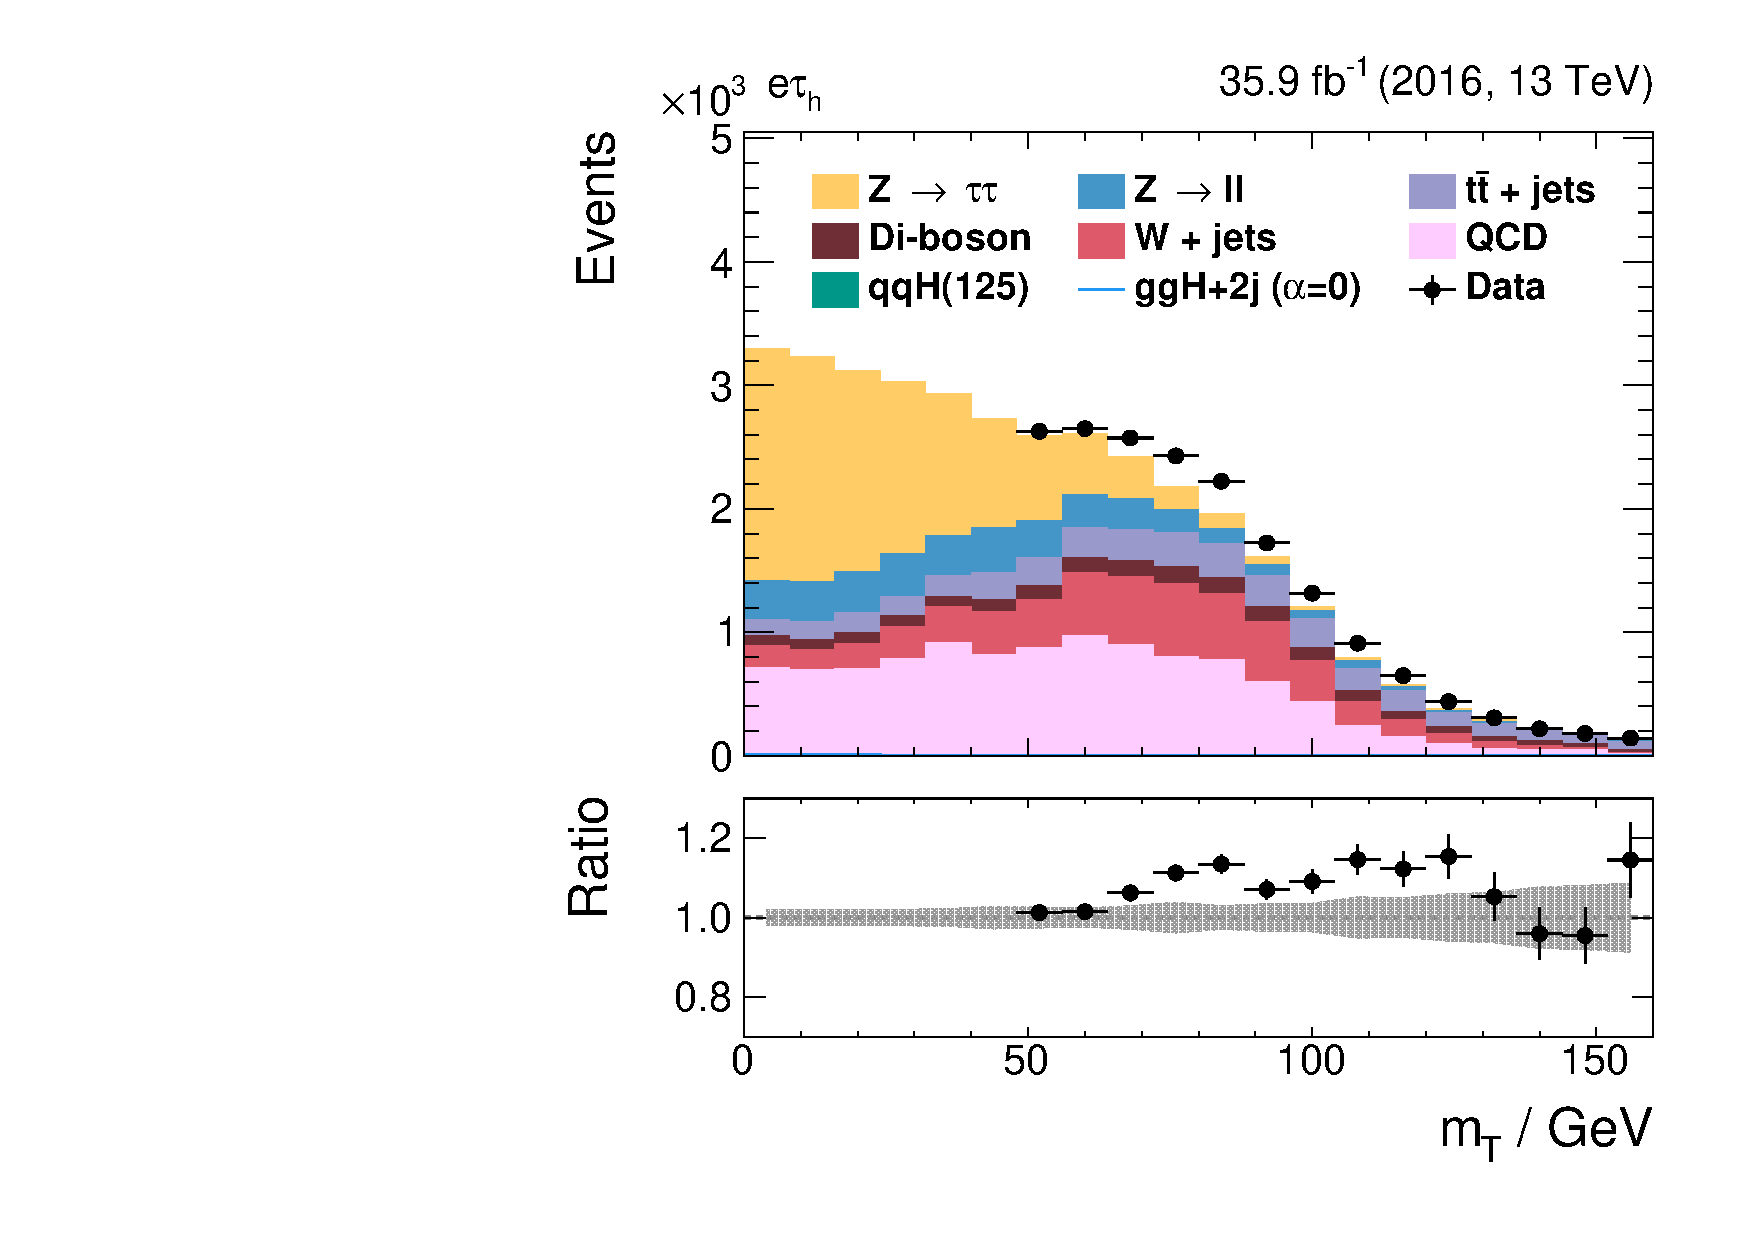
\includegraphics[width=0.47\textwidth]{Figures/background_estimation/control_plots/et/BoostedCP/mt_1.pdf}
  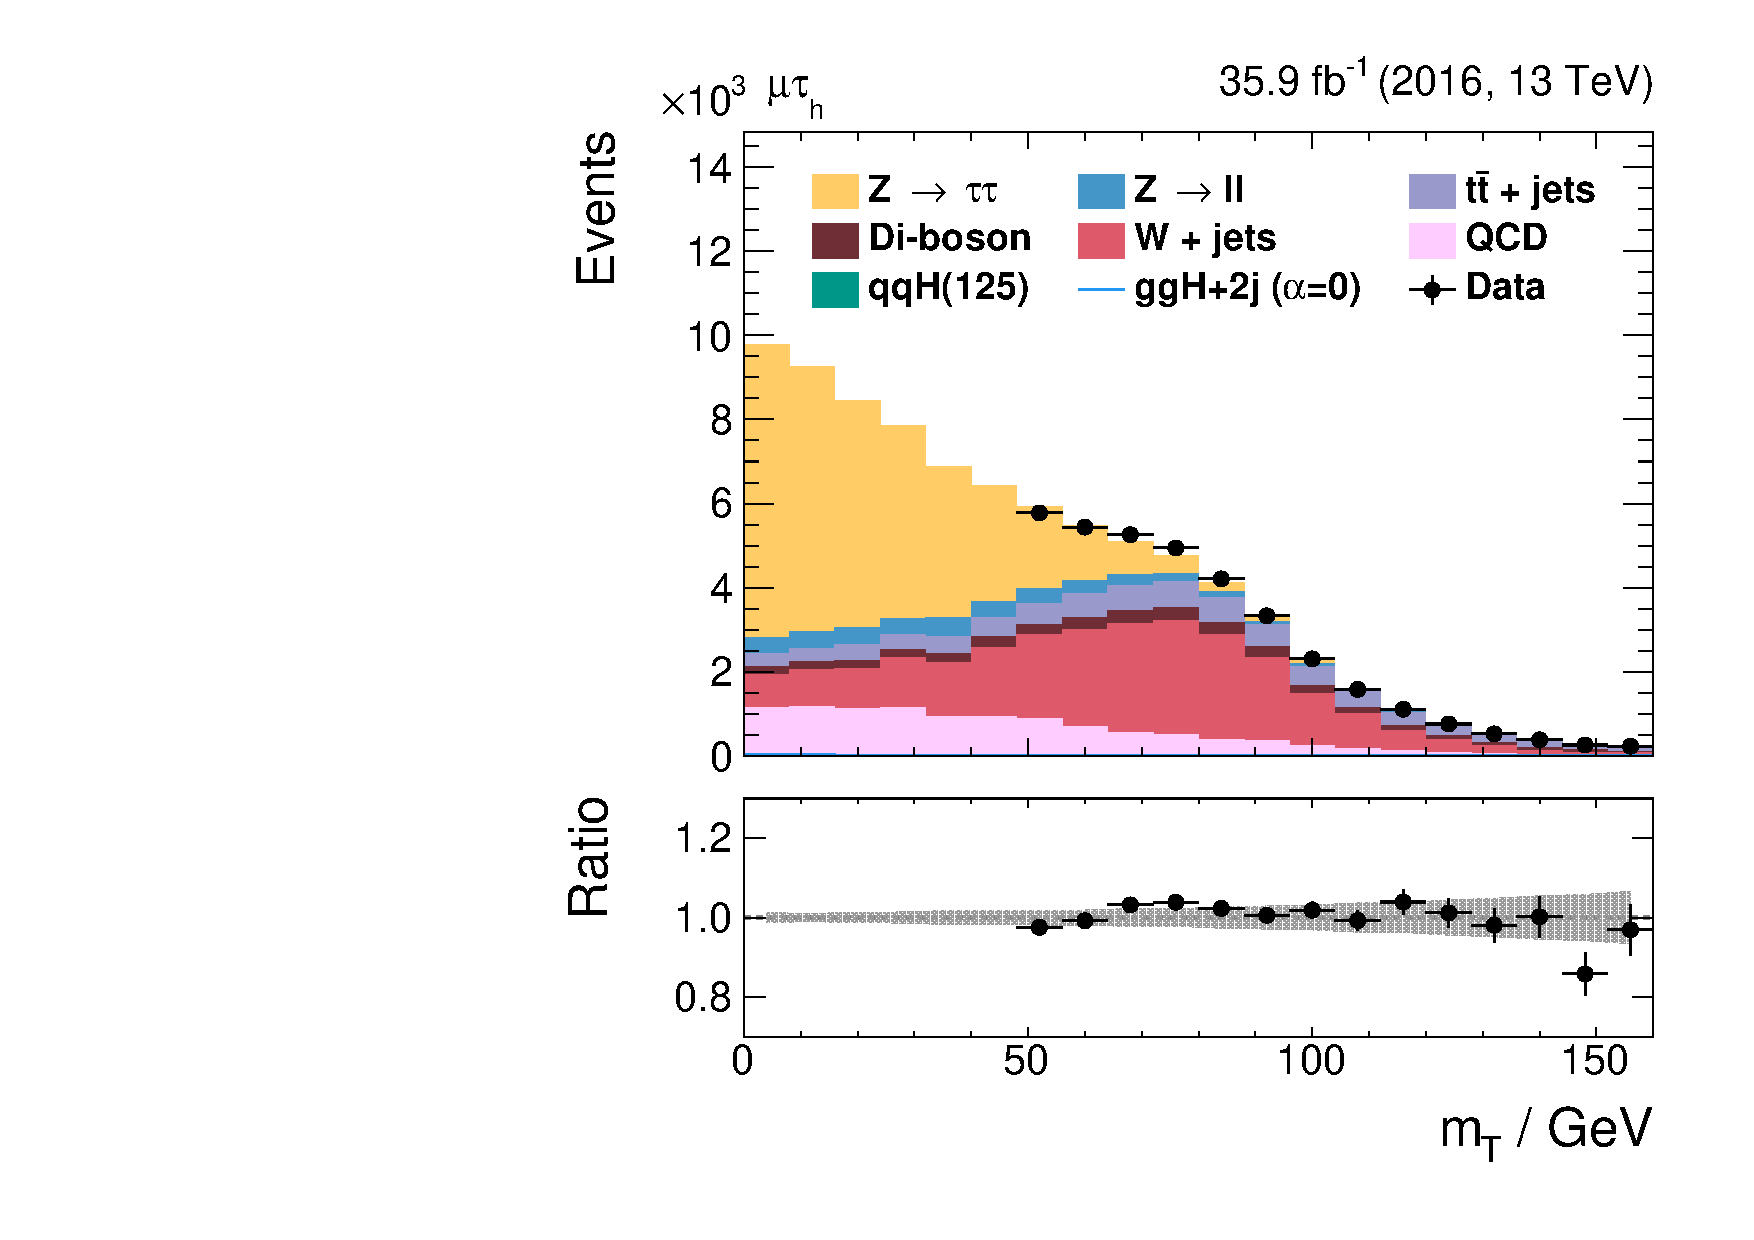
\includegraphics[width=0.47\textwidth]{Figures/background_estimation/control_plots/mt/BoostedCP/mt_1.pdf}
 \caption[\textit{W+jets} control plots in the \textit{boosted} category.]{Blinded $m_\text{T}$ distribution in the \textit{boosted} category for the $e\tau_\text{h}$ (left) and $\mu\tau_\text{h}$ (right) channel.
 Backgrounds were estimated with the techniques introduced in section \ref{sec:background_estimation}.}\label{fig:etmt_wj:wj_control_1jet}
\end{figure}

\begin{figure}[h!]
 \centering
  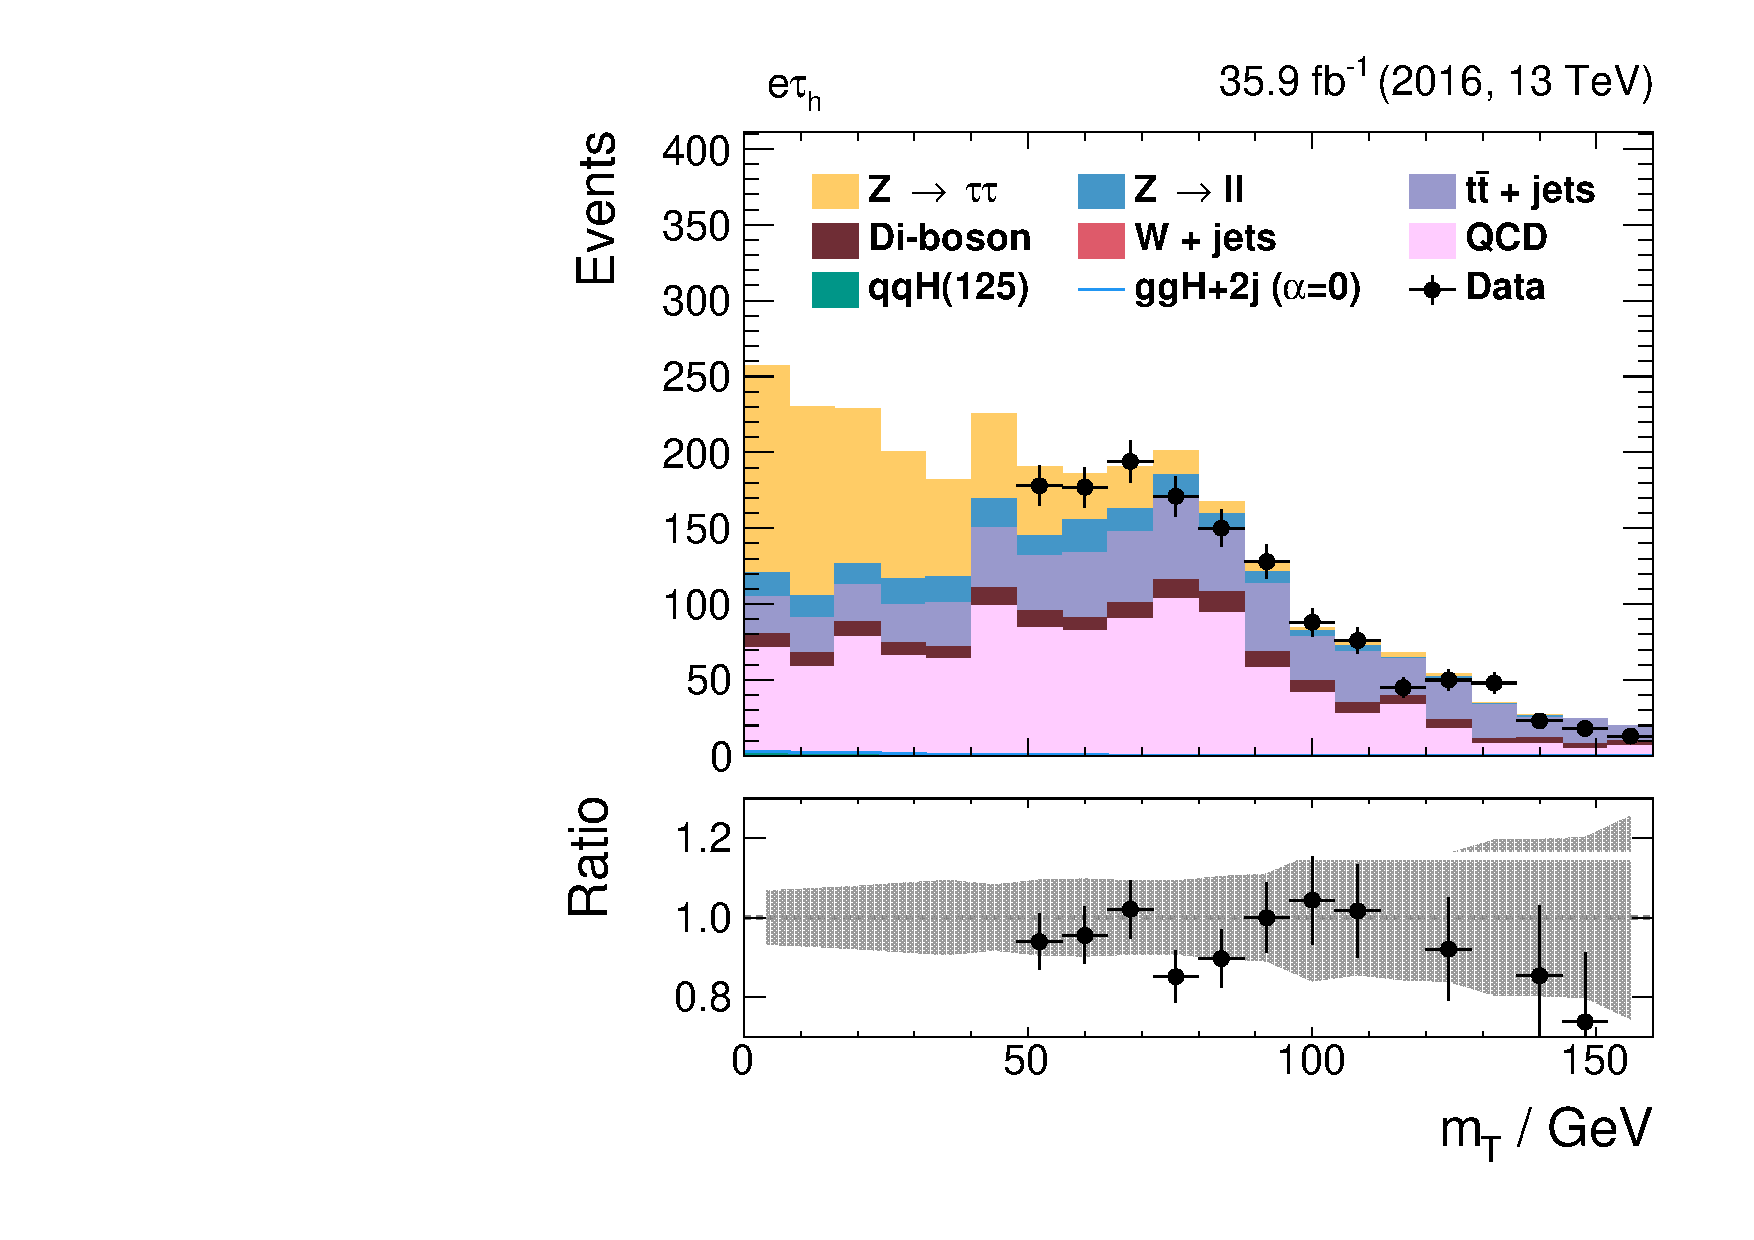
\includegraphics[width=0.47\textwidth]{Figures/background_estimation/control_plots/et/dijet2D_lowboost/mt_1.pdf}
  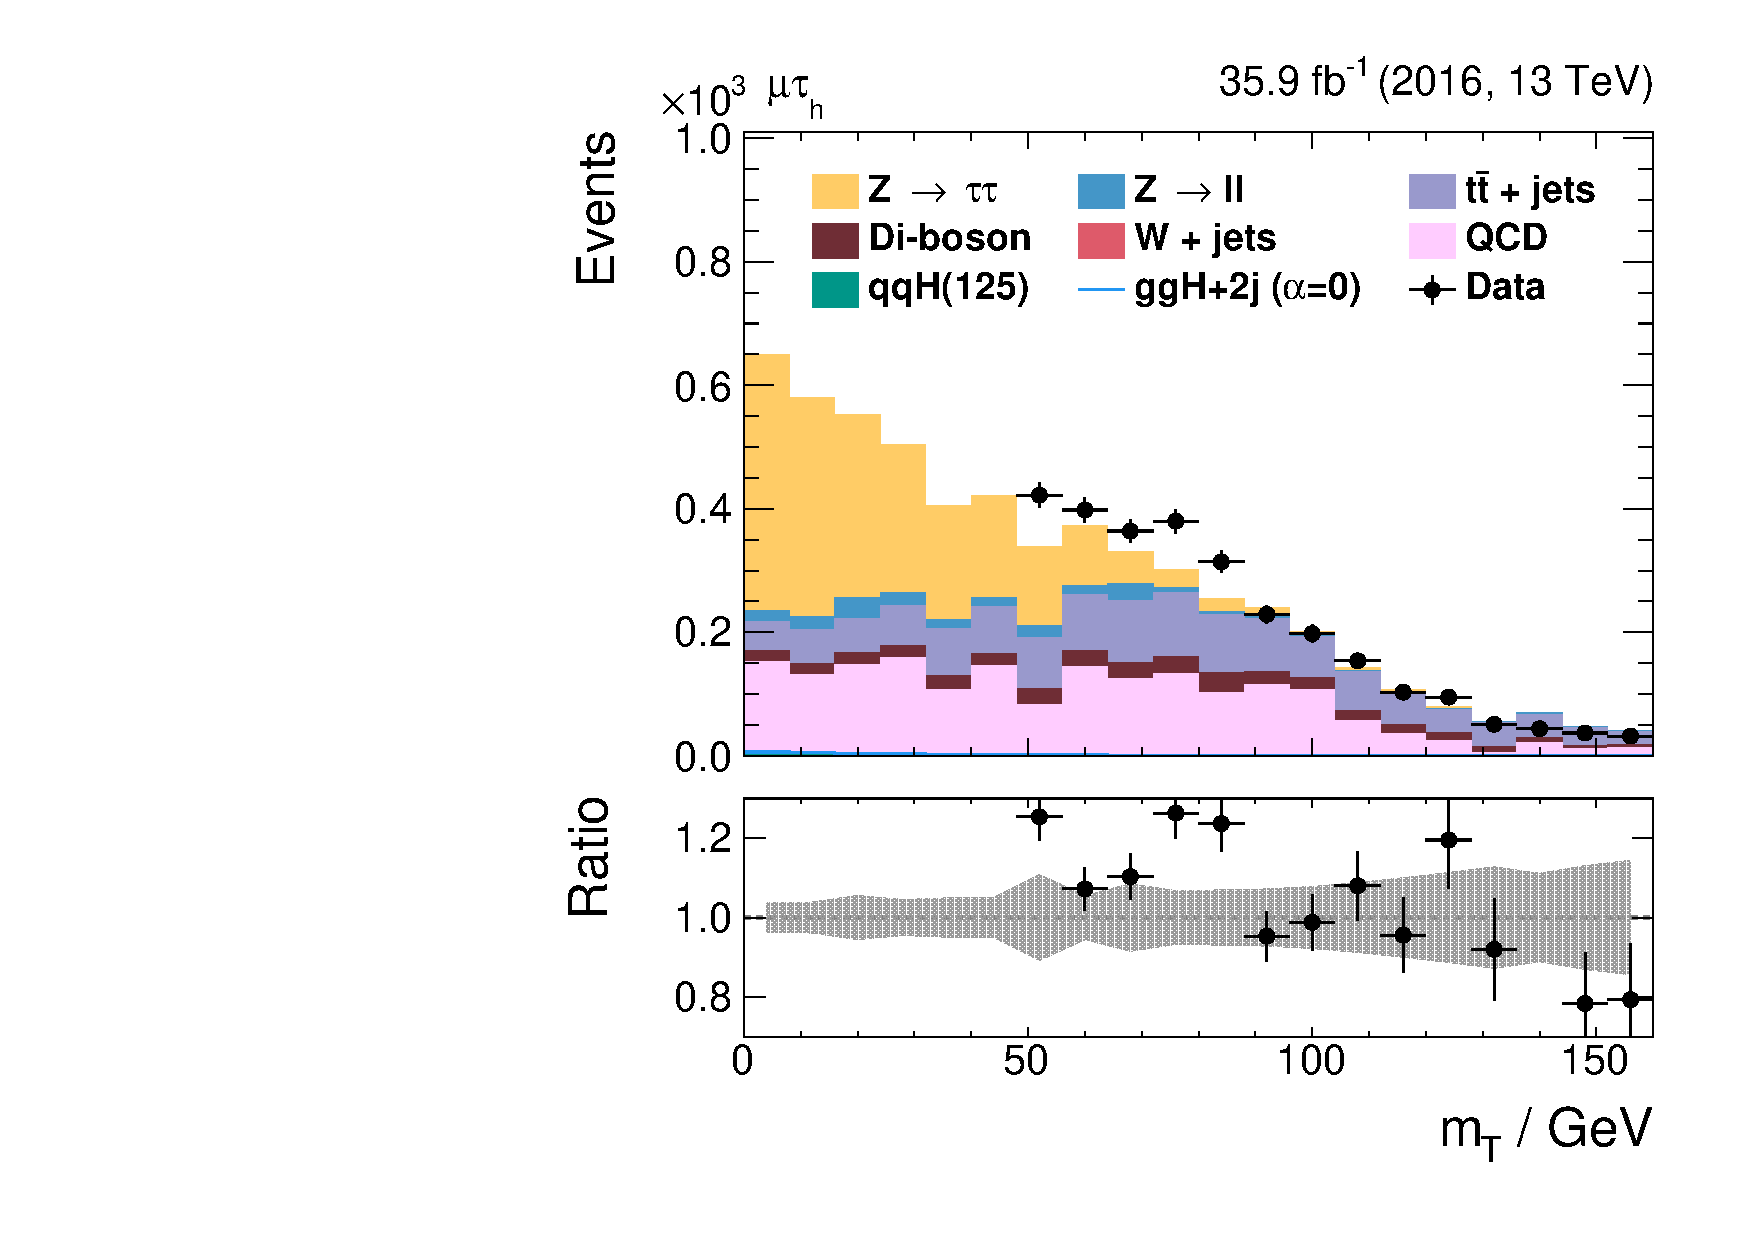
\includegraphics[width=0.47\textwidth]{Figures/background_estimation/control_plots/mt/dijet2D_lowboost/mt_1.pdf}  
\caption[\textit{W+jets} control plots in the \textit{dijet lowboost} category.]{Blinded $m_\text{T}$ distribution in the \textit{dijet lowboost} category for the $e\tau_\text{h}$ (left) and $\mu\tau_\text{h}$ (right) channel.
Backgrounds were estimated with the techniques introduced in section \ref{sec:background_estimation}.}\label{fig:etmt_wj:wj_control_lowboost}
\end{figure} 
\begin{figure}[h!]
    \centering
  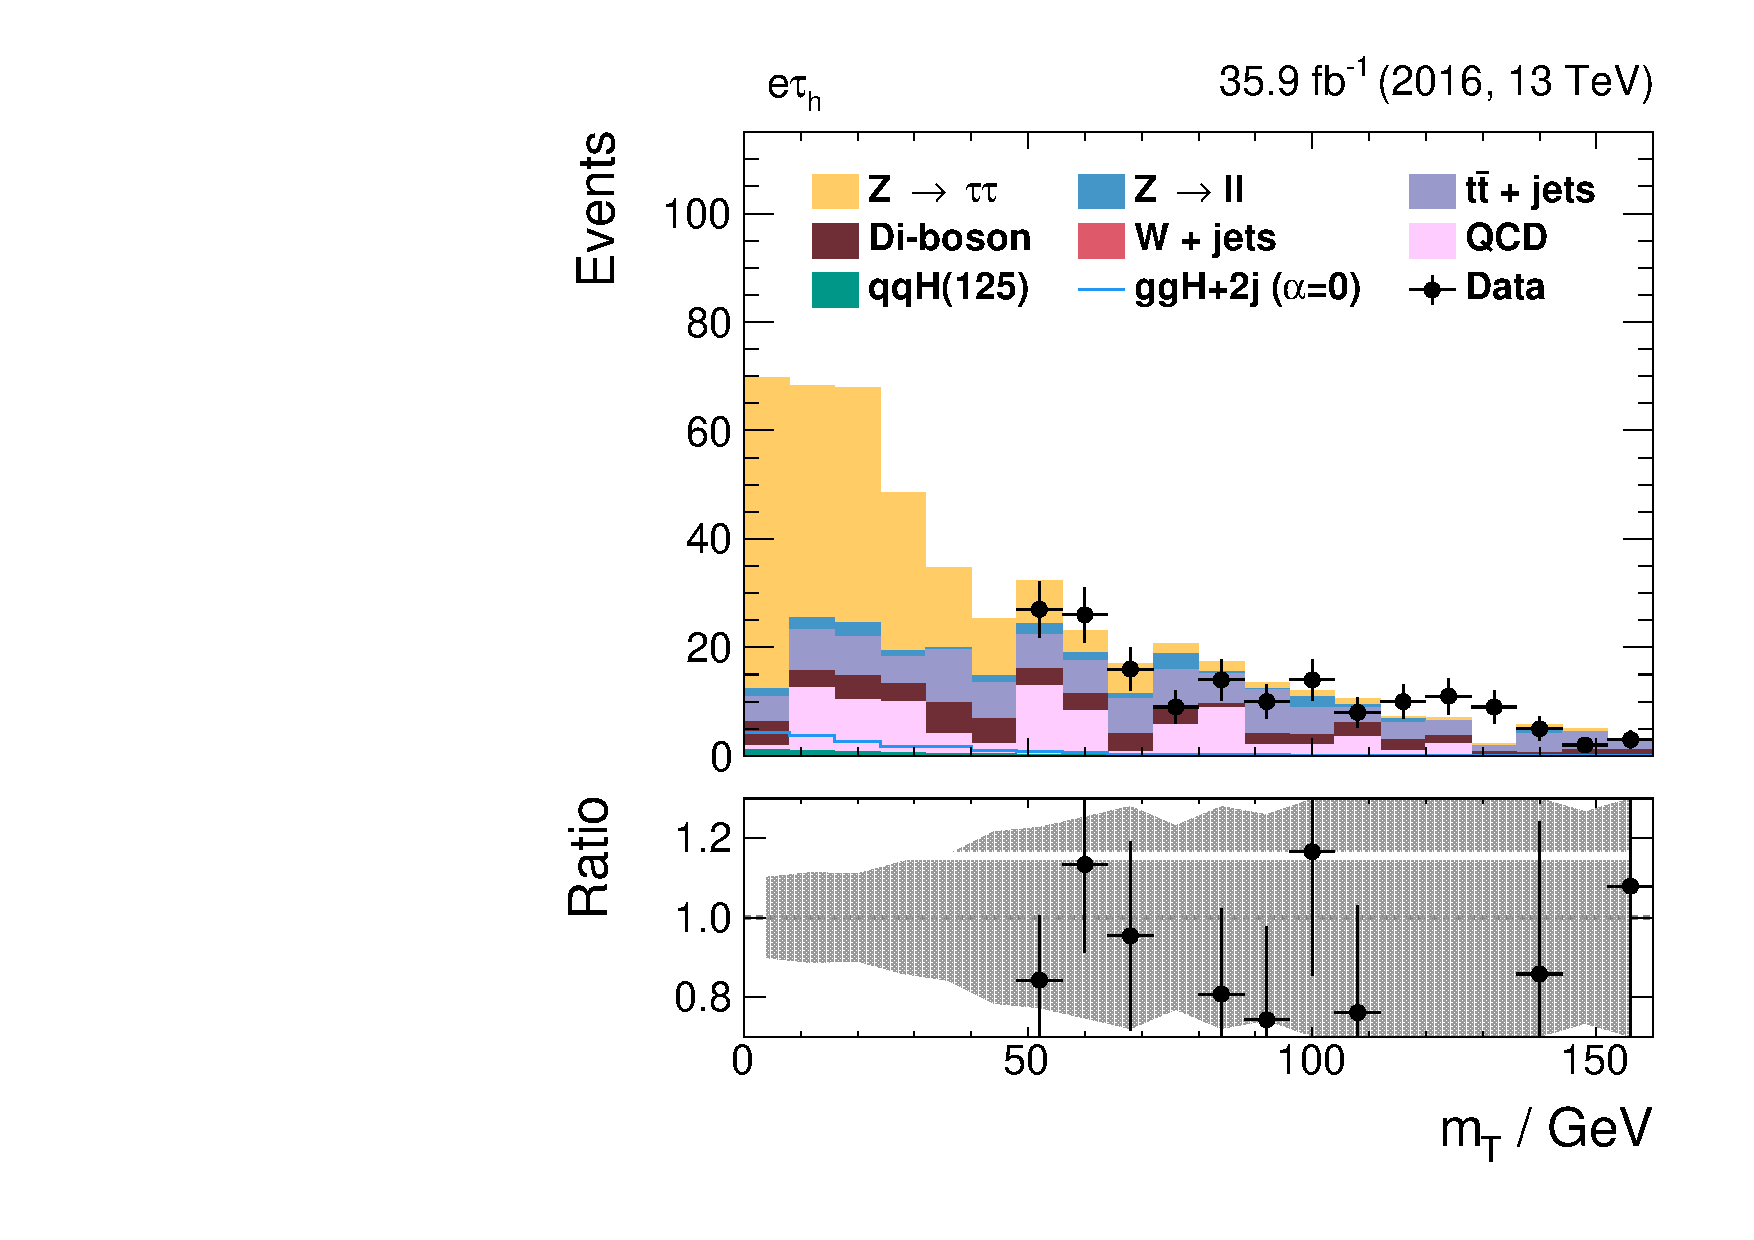
\includegraphics[width=0.47\textwidth]{Figures/background_estimation/control_plots/et/dijet2D_boosted/mt_1.pdf}
  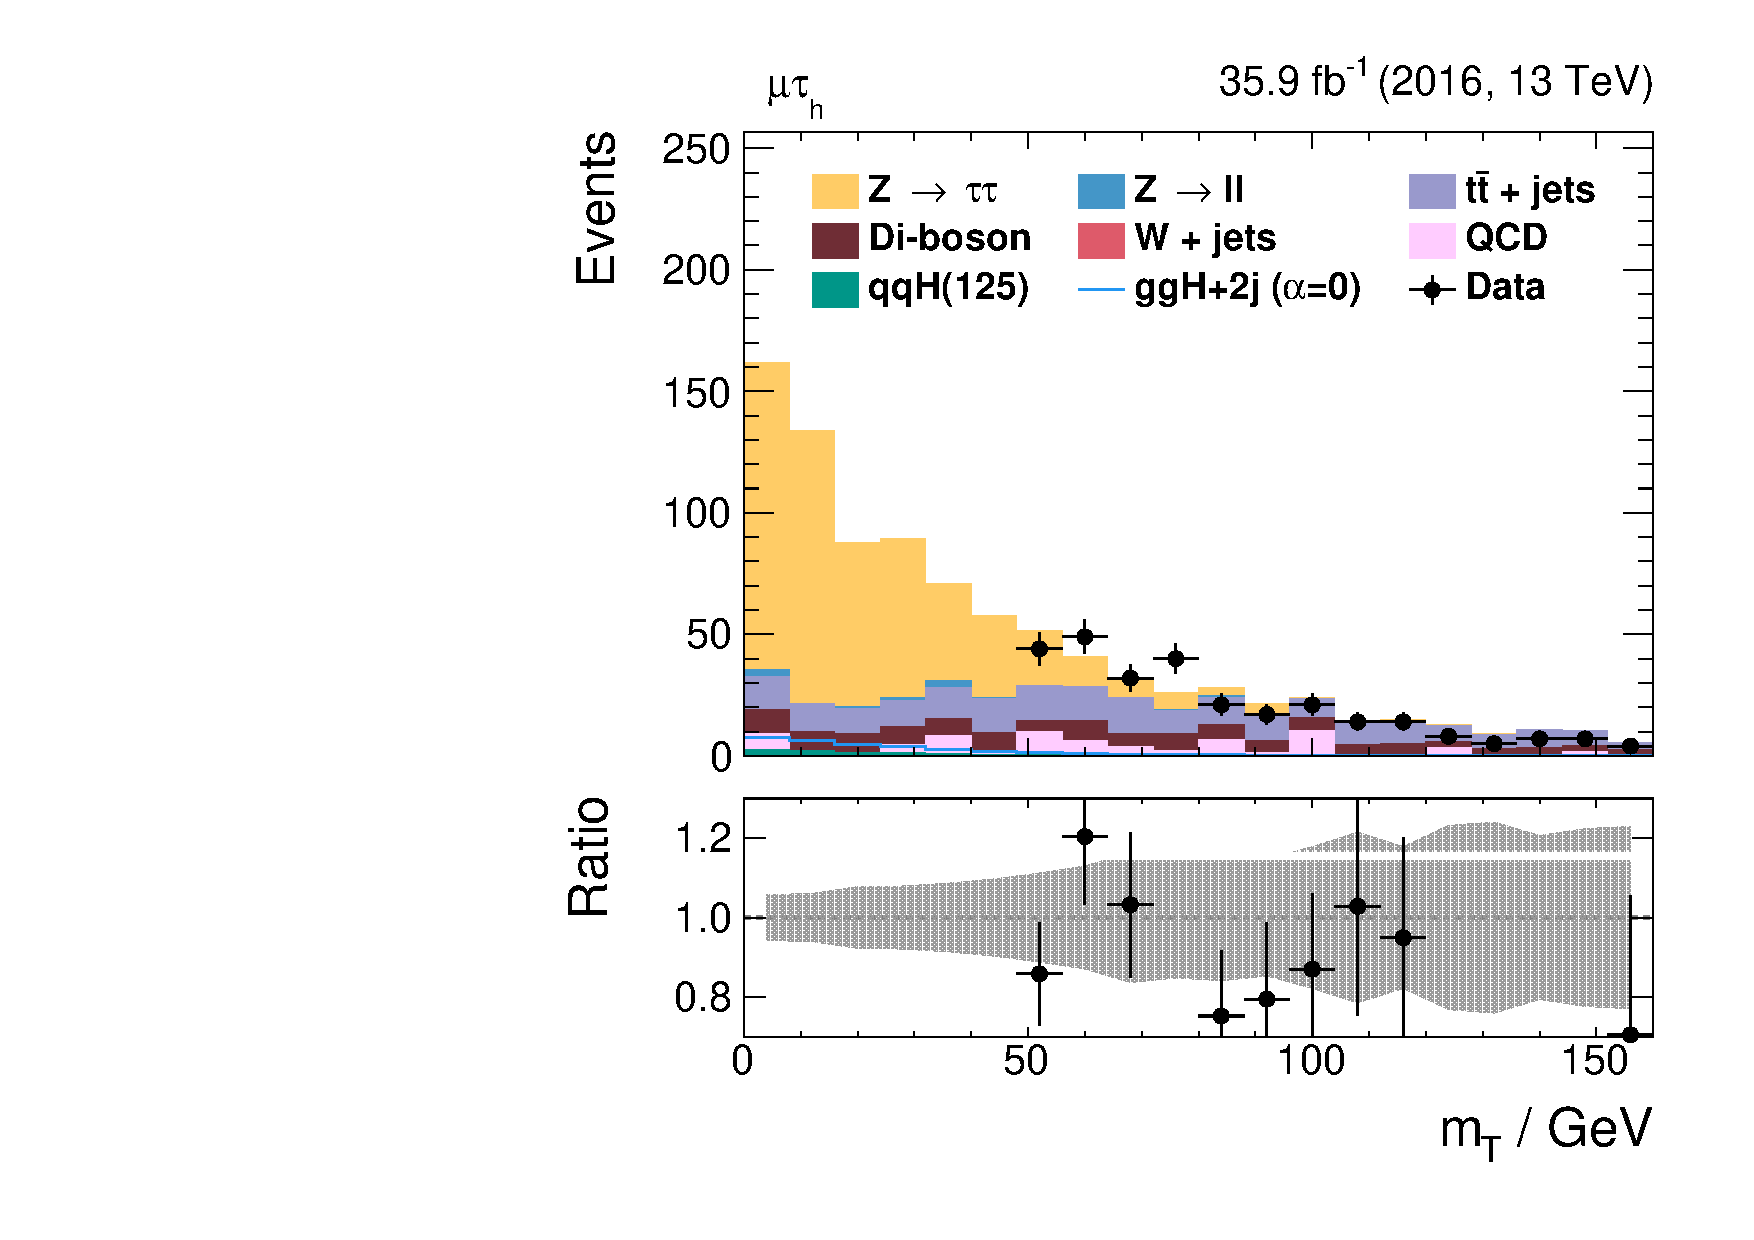
\includegraphics[width=0.47\textwidth]{Figures/background_estimation/control_plots/mt/dijet2D_boosted/mt_1.pdf} 
 \caption[\textit{W+jets} control plots in the \textit{dijet boosted} category.]{Blinded $m_\text{T}$ distribution in the \textit{dijet boosted} category for the  $e\tau_\text{h}$ (left) and $\mu\tau_\text{h}$  (right) channel.
 Backgrounds were estimated with the techniques introduced in section \ref{sec:background_estimation}.}\label{fig:etmt_wj:wj_control_boosted}
\end{figure}%
\clearpage 

\paragraph{W+jets control regions}\mbox{} \\ 
One OS high $m_\text{T}$ and one SS high $m_\text{T}$ control region are added to the final fit in the \textit{0-jet} and \textit{boosted} categories, respectively. As no \textit{W+jets} events remain in the SS high $m_\text{T}$ CR of the two dijet category, no dijet control regions are added to the final fit. 
This means in total eight \textit{W+jets} control regions are used with this setup.
The expected background contents and event numbers in these control regions are shown in figures \ref{fig:etmtqcd:0jet_w_control} and \ref{fig:etmtqcd:0jet_w_ss_control} for the high $m_\text{T}$ and SS high $m_\text{T}$ region, respectively.

% HiggsAnalysis/KITHiggsToTauTau/scripts/makePlots_prefitPostfitPlots.py -i CombineHarvester/HTTSMCP2016/output/2018-09-23_FULL_mela3D_JECgroupings/et/common/htt_inputet10.root -b ZTT "ZLL ZL ZJ" "TT TTT TTJ" "VV VVT VVJ" W QCD qqH -r -a " --y-subplot-lims 0.95 1.05 --x-label \"m_{#tau#tau} / GeV\" --y-label \"Events/bin\"  --title \"e#tau_{h} - 0jet W CR\" --formats pdf png " --www qcd_et_control-regions --cpggh
% HiggsAnalysis/KITHiggsToTauTau/scripts/makePlots_prefitPostfitPlots.py -i CombineHarvester/HTTSMCP2016/output/2018-09-23_FULL_mela3D_JECgroupings/et/common/htt_inputet11.root -b ZTT "ZLL ZL ZJ" "TT TTT TTJ" "VV VVT VVJ" W QCD qqH -r -a " --y-subplot-lims 0.9 1.1 --x-label \"m_{#tau#tau} / GeV\" --y-label \"Events/bin\"  --title \"e#tau_{h} - 0jet QCD CR\" --formats pdf png " --www qcd_et_control-regions --cpggh
% HiggsAnalysis/KITHiggsToTauTau/scripts/makePlots_prefitPostfitPlots.py -i CombineHarvester/HTTSMCP2016/output/2018-09-23_FULL_mela3D_JECgroupings/et/common/htt_inputet12.root -b ZTT "ZLL ZL ZJ" "TT TTT TTJ" "VV VVT VVJ" W QCD qqH -r -a " --y-subplot-lims 0.95 1.05 --x-label \"m_{#tau#tau} / GeV\" --y-label \"Events/bin\"  --title \"e#tau_{h} - 0jet W SS CR\" --formats pdf png " --www qcd_et_control-regions --cpggh
% HiggsAnalysis/KITHiggsToTauTau/scripts/makePlots_prefitPostfitPlots.py -i CombineHarvester/HTTSMCP2016/output/2018-09-23_FULL_mela3D_JECgroupings/et/common/htt_inputet13.root -b ZTT "ZLL ZL ZJ" "TT TTT TTJ" "VV VVT VVJ" W QCD qqH -r -a " --y-subplot-lims 0.95 1.05 --x-label \"m_{#tau#tau} / GeV\" --y-label \"Events/bin\"  --title \"e#tau_{h} - boosted W CR\" --formats pdf png " --www qcd_et_control-regions --cpggh
% HiggsAnalysis/KITHiggsToTauTau/scripts/makePlots_prefitPostfitPlots.py -i CombineHarvester/HTTSMCP2016/output/2018-09-23_FULL_mela3D_JECgroupings/et/common/htt_inputet14.root -b ZTT "ZLL ZL ZJ" "TT TTT TTJ" "VV VVT VVJ" W QCD qqH -r -a " --y-subplot-lims 0.95 1.05 --x-label \"m_{#tau#tau} / GeV\" --y-label \"Events/bin\"  --title \"e#tau_{h} - boosted QCD CR\" --formats pdf png "  --www qcd_et_control-regions --cpggh
% HiggsAnalysis/KITHiggsToTauTau/scripts/makePlots_prefitPostfitPlots.py -i CombineHarvester/HTTSMCP2016/output/2018-09-23_FULL_mela3D_JECgroupings/et/common/htt_inputet15.root -b ZTT "ZLL ZL ZJ" "TT TTT TTJ" "VV VVT VVJ" W QCD qqH -r -a " --y-subplot-lims 0.95 1.05 --x-label \"m_{#tau#tau} / GeV\" --y-label \"Events/bin\"  --title \"e#tau_{h} - boosted W SS CR\" --formats pdf png "  --www qcd_et_control-regions --cpggh
% HiggsAnalysis/KITHiggsToTauTau/scripts/makePlots_prefitPostfitPlots.py -i CombineHarvester/HTTSMCP2016/output/2018-09-23_FULL_mela3D_JECgroupings/mt/common/htt_inputmt10.root -b ZTT "ZLL ZL ZJ" "TT TTT TTJ" "VV VVT VVJ" W QCD qqH -r -a " --y-subplot-lims 0.95 1.05 --x-label \"m_{#tau#tau} / GeV\" --y-label \"Events/bin\"  --title \"#mu#tau_{h} - 0jet W CR\" --formats pdf png " --www qcd_mt_control-regions --cpggh
% HiggsAnalysis/KITHiggsToTauTau/scripts/makePlots_prefitPostfitPlots.py -i CombineHarvester/HTTSMCP2016/output/2018-09-23_FULL_mela3D_JECgroupings/mt/common/htt_inputmt11.root -b ZTT "ZLL ZL ZJ" "TT TTT TTJ" "VV VVT VVJ" W QCD qqH -r -a " --y-subplot-lims 0.9 1.1 --x-label \"m_{#tau#tau} / GeV\" --y-label \"Events/bin\"  --title \"#mu#tau_{h} - 0jet QCD CR\" --formats pdf png " --www qcd_mt_control-regions --cpggh
% HiggsAnalysis/KITHiggsToTauTau/scripts/makePlots_prefitPostfitPlots.py -i CombineHarvester/HTTSMCP2016/output/2018-09-23_FULL_mela3D_JECgroupings/mt/common/htt_inputmt12.root -b ZTT "ZLL ZL ZJ" "TT TTT TTJ" "VV VVT VVJ" W QCD qqH -r -a " --y-subplot-lims 0.95 1.05 --x-label \"m_{#tau#tau} / GeV\" --y-label \"Events/bin\"  --title \"#mu#tau_{h} - 0jet W SS CR\" --formats pdf png " --www qcd_mt_control-regions --cpggh
% HiggsAnalysis/KITHiggsToTauTau/scripts/makePlots_prefitPostfitPlots.py -i CombineHarvester/HTTSMCP2016/output/2018-09-23_FULL_mela3D_JECgroupings/mt/common/htt_inputmt13.root -b ZTT "ZLL ZL ZJ" "TT TTT TTJ" "VV VVT VVJ" W QCD qqH -r -a " --y-subplot-lims 0.95 1.05 --x-label \"m_{#tau#tau} / GeV\" --y-label \"Events/bin\"  --title \"#mu#tau_{h} - boosted W CR\" --formats pdf png " --www qcd_mt_control-regions --cpggh
% HiggsAnalysis/KITHiggsToTauTau/scripts/makePlots_prefitPostfitPlots.py -i CombineHarvester/HTTSMCP2016/output/2018-09-23_FULL_mela3D_JECgroupings/mt/common/htt_inputmt14.root -b ZTT "ZLL ZL ZJ" "TT TTT TTJ" "VV VVT VVJ" W QCD qqH -r -a " --y-subplot-lims 0.9 1.1 --x-label \"m_{#tau#tau} / GeV\" --y-label \"Events/bin\"  --title \"#mu#tau_{h} - boosted QCD CR\" --formats pdf png "  --www qcd_mt_control-regions --cpggh
% HiggsAnalysis/KITHiggsToTauTau/scripts/makePlots_prefitPostfitPlots.py -i CombineHarvester/HTTSMCP2016/output/2018-09-23_FULL_mela3D_JECgroupings/mt/common/htt_inputmt15.root -b ZTT "ZLL ZL ZJ" "TT TTT TTJ" "VV VVT VVJ" W QCD qqH -r -a " --y-subplot-lims 0.95 1.05 --x-label \"m_{#tau#tau} / GeV\" --y-label \"Events/bin\"  --title \"#mu#tau_{h} - boosted W SS CR\" --formats pdf png "  --www qcd_mt_control-regions --cpggh
% HiggsAnalysis/KITHiggsToTauTau/scripts/makePlots_prefitPostfitPlots.py -i CombineHarvester/HTTSMCP2016/output/2018-09-23_FULL_mela3D_JECgroupings/et/common/htt_inputet17.root -b ZTT "ZLL ZL ZJ" "TT TTT TTJ" "VV VVT VVJ" W QCD qqH -r -a " --y-subplot-lims 0.9 1.1 --x-label \"m_{#tau#tau} / GeV\" --y-label \"Events/bin\"  --title \"e#tau_{h}-2jet lowboost QCD CR\" --formats pdf png "  --www qcd_et_control-regions --cpggh
% HiggsAnalysis/KITHiggsToTauTau/scripts/makePlots_prefitPostfitPlots.py -i CombineHarvester/HTTSMCP2016/output/2018-09-23_FULL_mela3D_JECgroupings/mt/common/htt_inputmt17.root -b ZTT "ZLL ZL ZJ" "TT TTT TTJ" "VV VVT VVJ" W QCD qqH -r -a " --y-subplot-lims 0.9 1.1 --x-label \"m_{#tau#tau} / GeV\" --y-label \"Events/bin\"  --title \"#mu#tau_{h}-2jet lowboost QCD CR\" --formats pdf png "  --www qcd_mt_control-regions --cpggh
% HiggsAnalysis/KITHiggsToTauTau/scripts/makePlots_prefitPostfitPlots.py -i CombineHarvester/HTTSMCP2016/output/2018-09-23_FULL_mela3D_JECgroupings/et/common/htt_inputet20.root -b ZTT "ZLL ZL ZJ" "TT TTT TTJ" "VV VVT VVJ" W QCD qqH -r -a " --y-subplot-lims 0.9 1.1 --x-label \"m_{#tau#tau} / GeV\" --y-label \"Events/bin\"  --title \"e#tau_{h}-2jet boosted QCD CR\" --formats pdf png "  --www qcd_et_control-regions --cpggh
% HiggsAnalysis/KITHiggsToTauTau/scripts/makePlots_prefitPostfitPlots.py -i CombineHarvester/HTTSMCP2016/output/2018-09-23_FULL_mela3D_JECgroupings/mt/common/htt_inputmt20.root -b ZTT "ZLL ZL ZJ" "TT TTT TTJ" "VV VVT VVJ" W QCD qqH -r -a " --y-subplot-lims 0.9 1.1 --x-label \"m_{#tau#tau} / GeV\" --y-label \"Events/bin\"  --title \"#mu#tau_{h}-2jet boosted QCD CR\" --formats pdf png "  --www qcd_mt_control-regions --cpggh

\begin{figure}[h!]
   \centering
  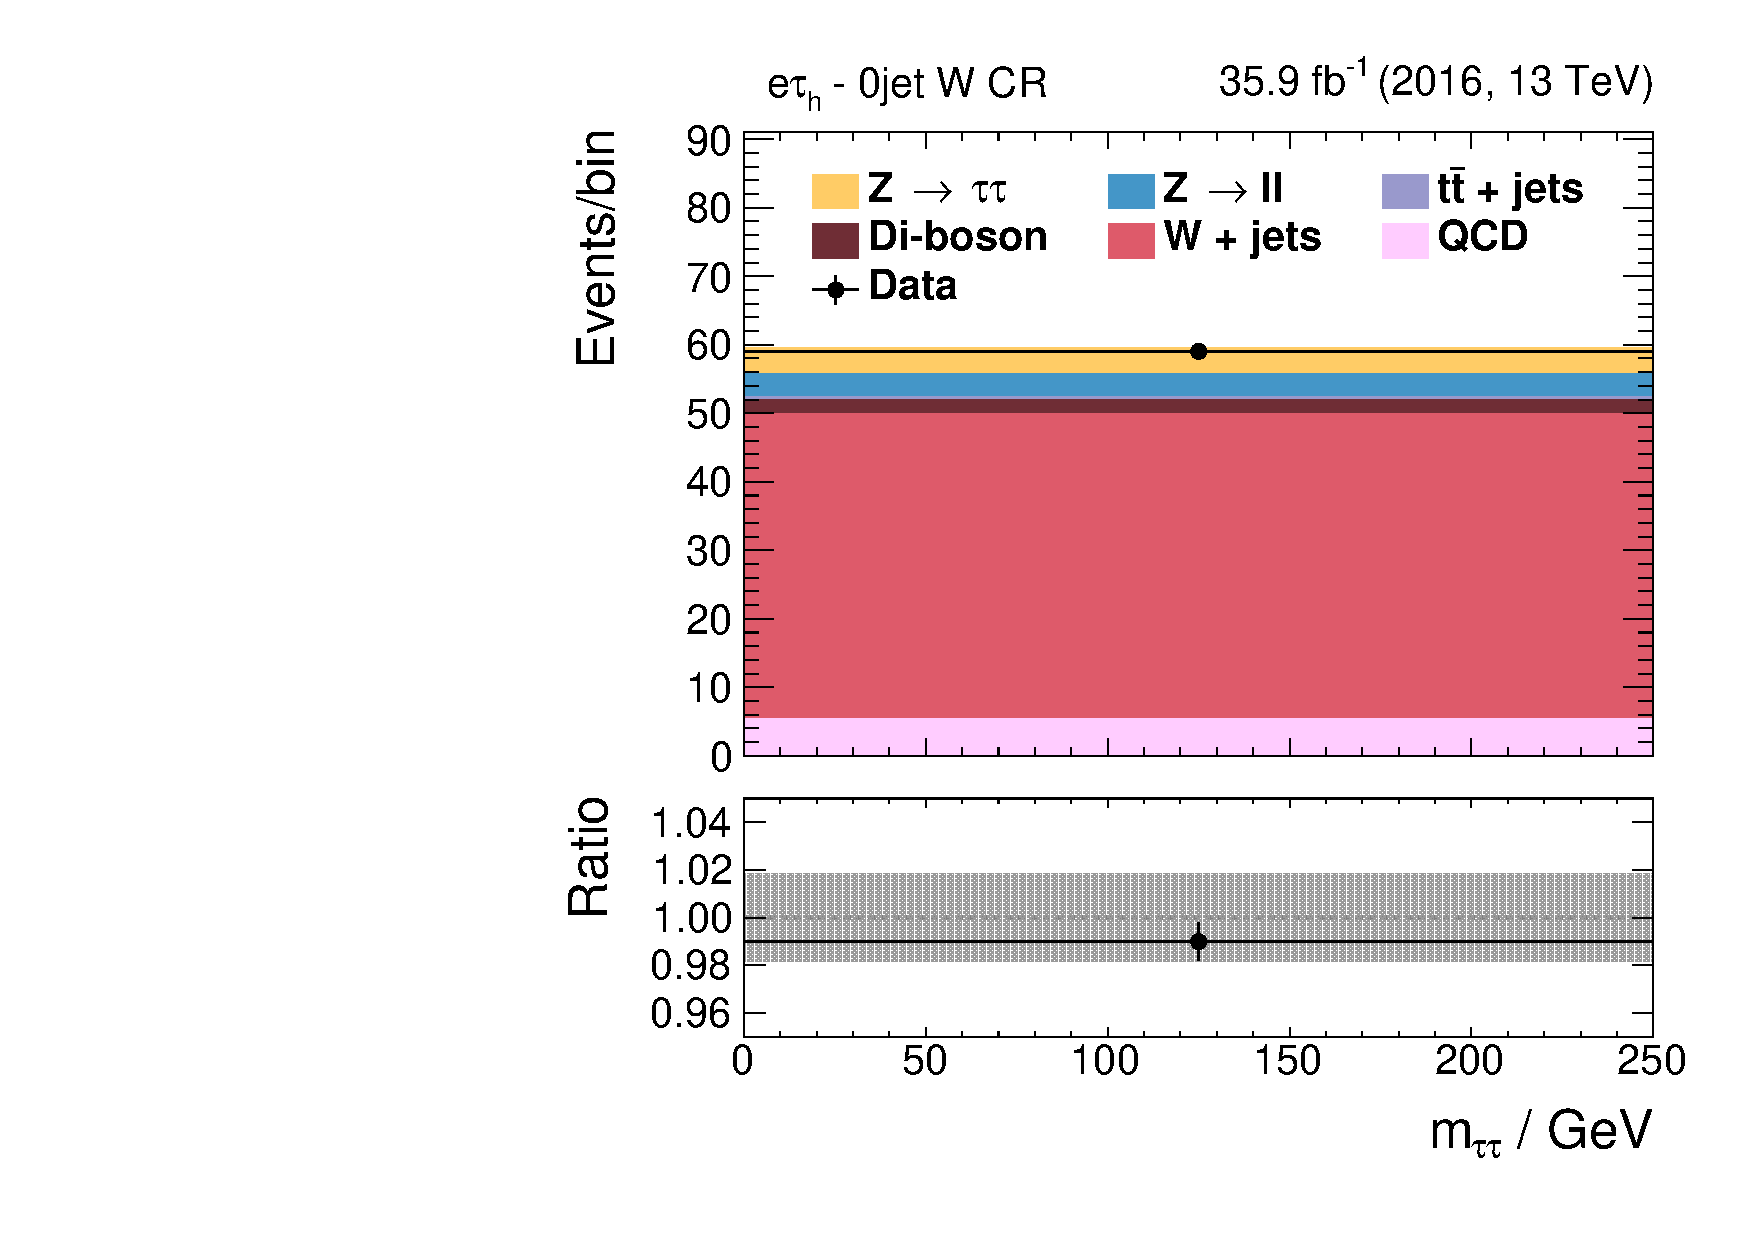
\includegraphics[width=0.47\textwidth]{Figures/background_estimation/qcd_et_control-regions/htt_inputet10__htt_et_10_13TeV.pdf}
  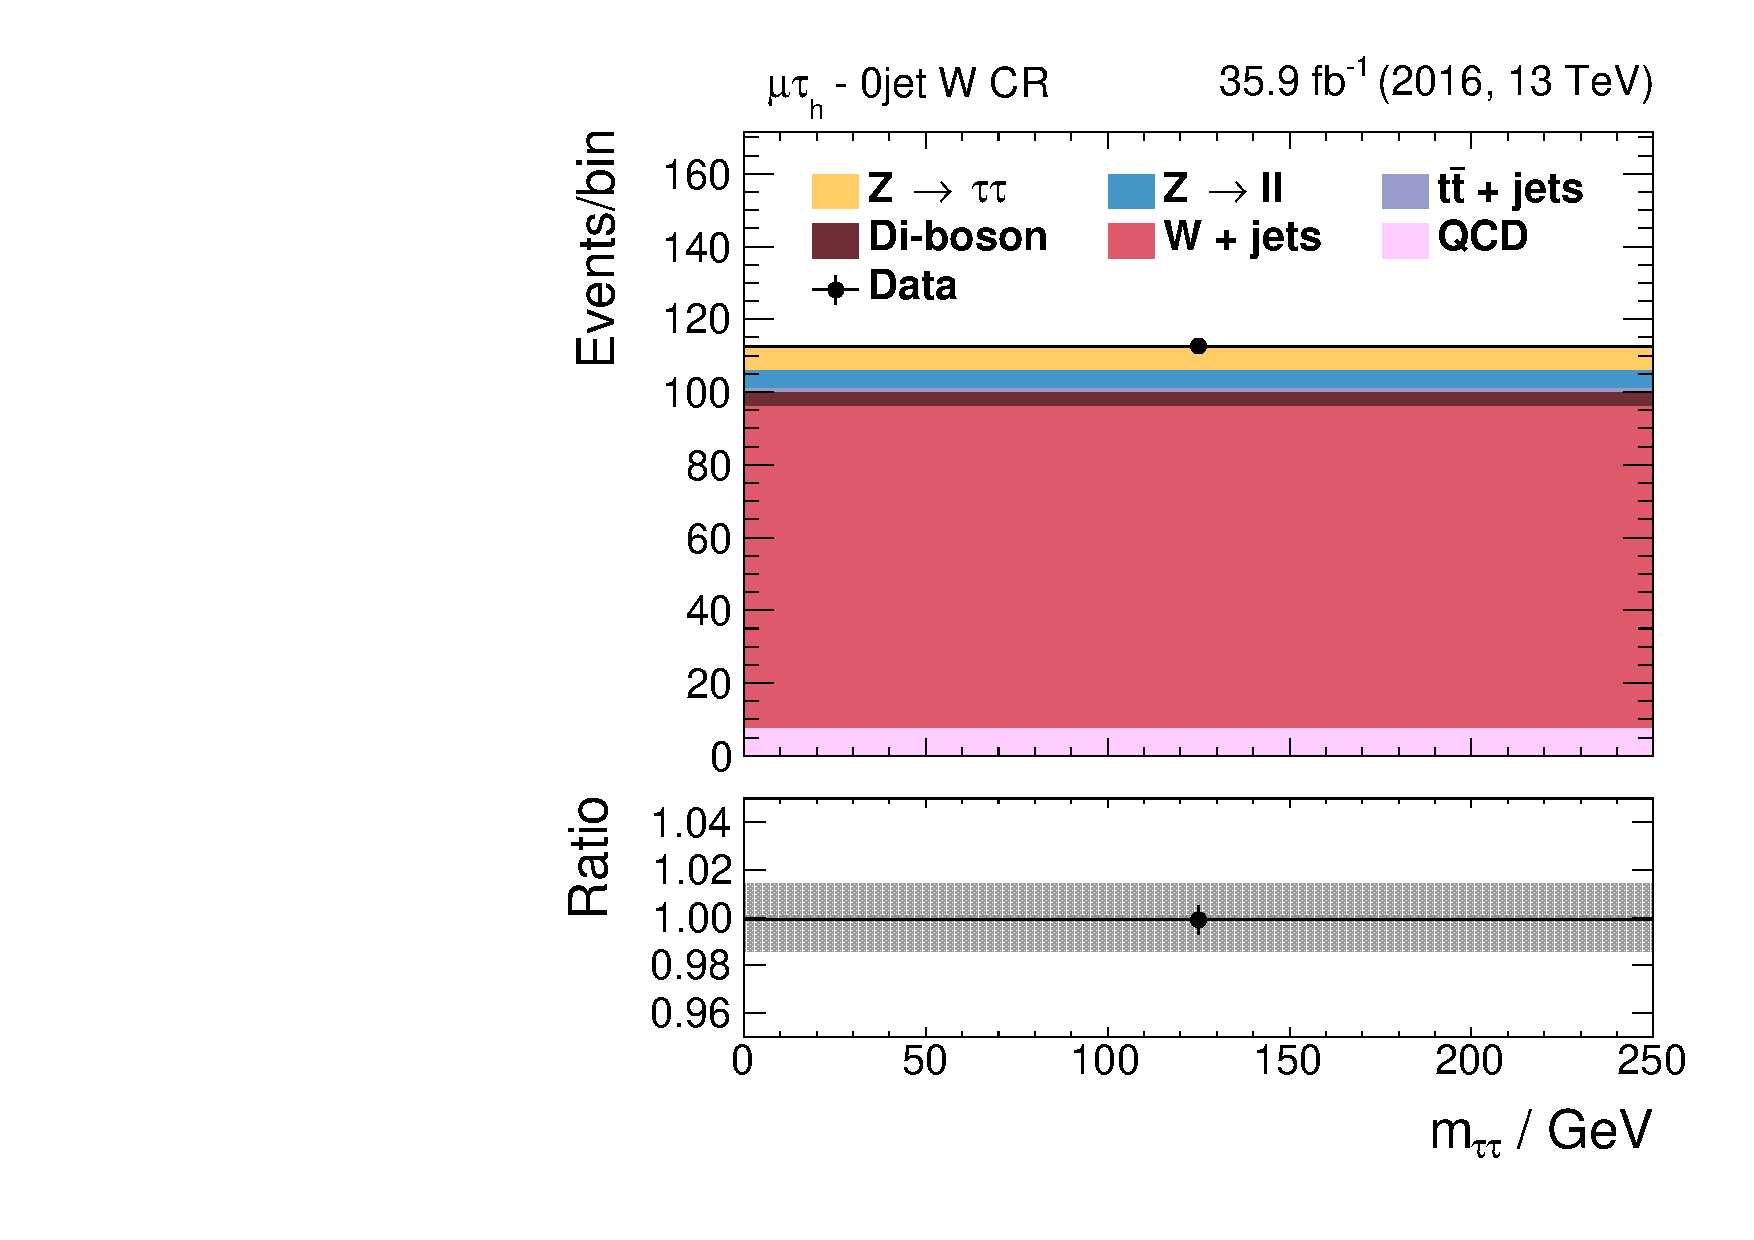
\includegraphics[width=0.47\textwidth]{Figures/background_estimation/qcd_mt_control-regions/htt_inputmt10__htt_mt_10_13TeV.pdf}
 \caption[\textit{0-jet} opposite-sign \textit{W+jets} control regions.]{Control region expected background normalization and data as given into the final fit for the W+jets OS high $m_\text{T}$ control region in the \textit{0-jet} category for the $e\tau_\text{h}$ (left) and $\mu\tau_\text{h}$ (right) channels.}\label{fig:etmtqcd:0jet_w_control}
\end{figure}

\begin{figure}[h!]
    \centering
    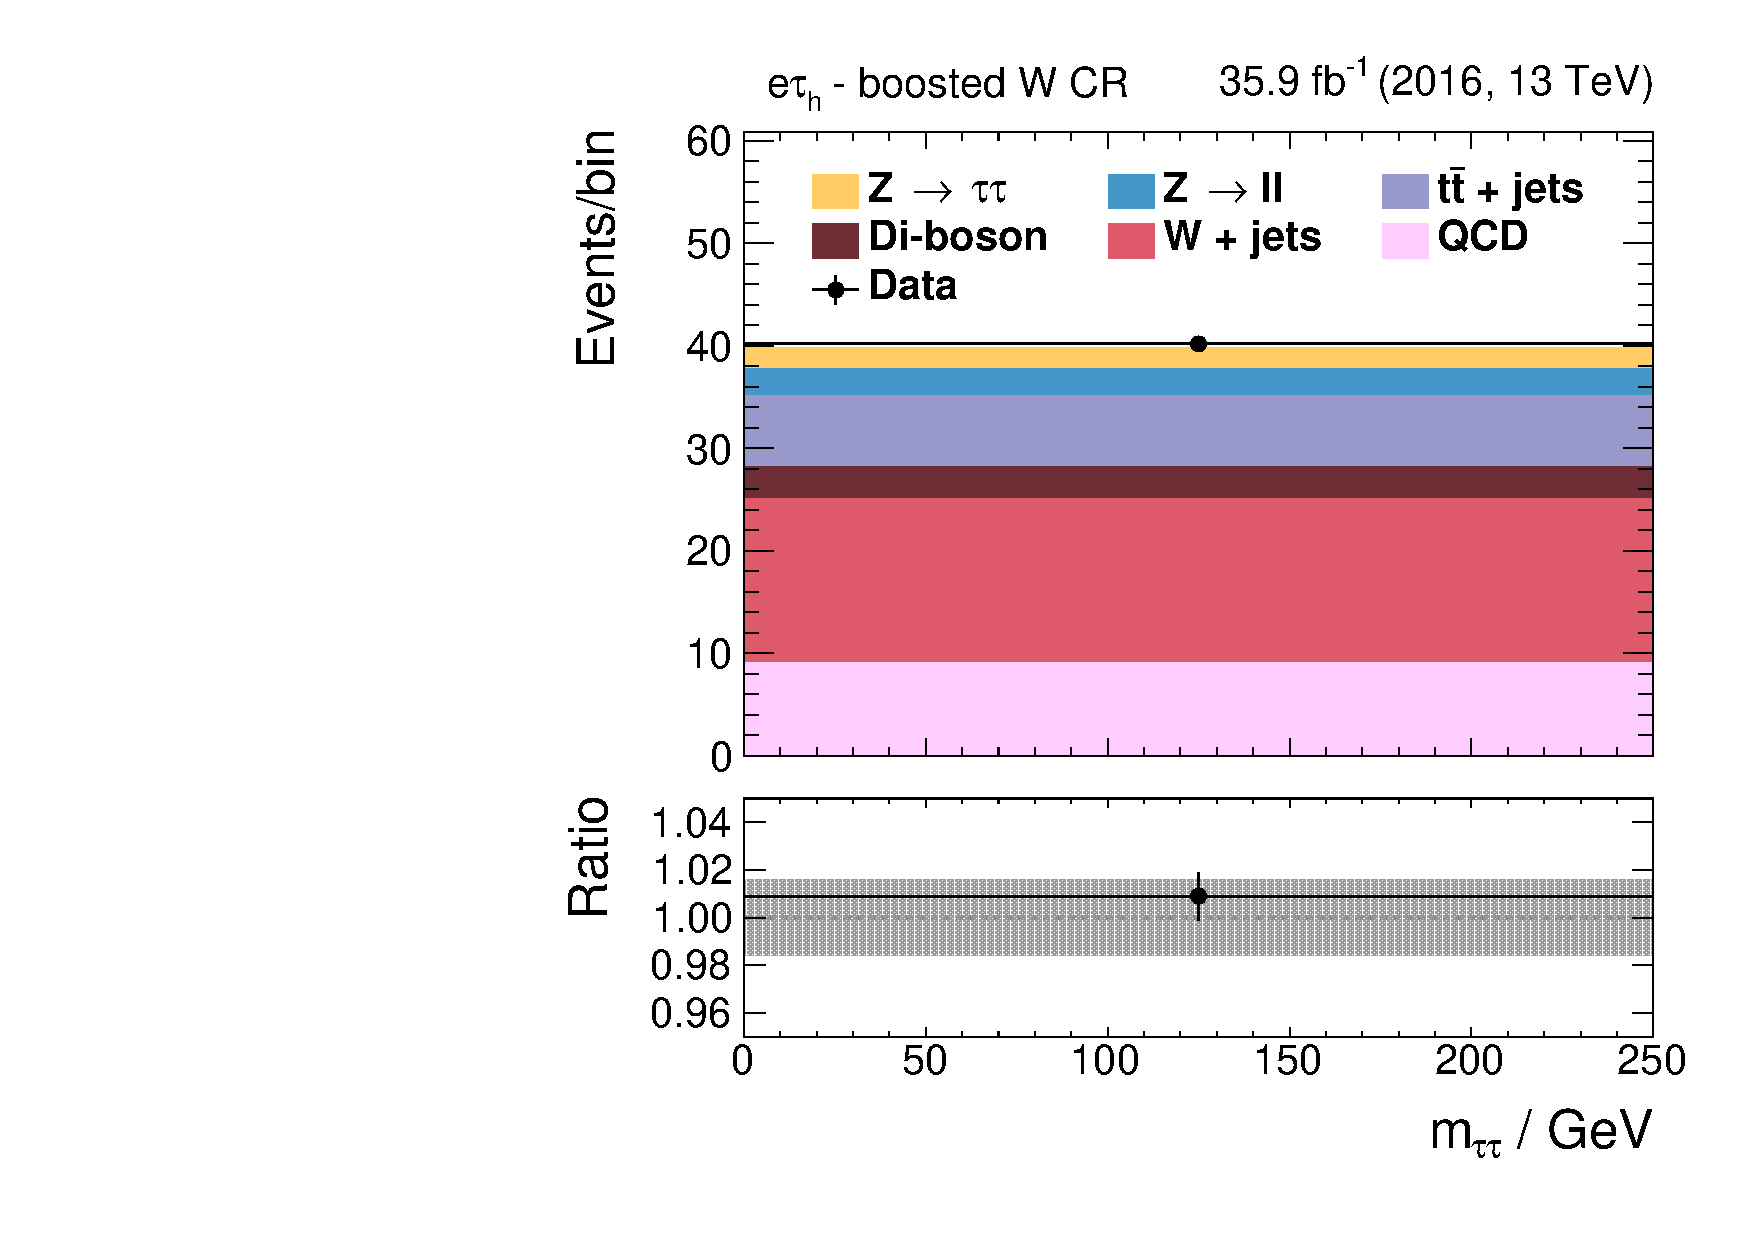
\includegraphics[width=0.47\textwidth]{Figures/background_estimation/qcd_et_control-regions/htt_inputet13__htt_et_13_13TeV.pdf}
    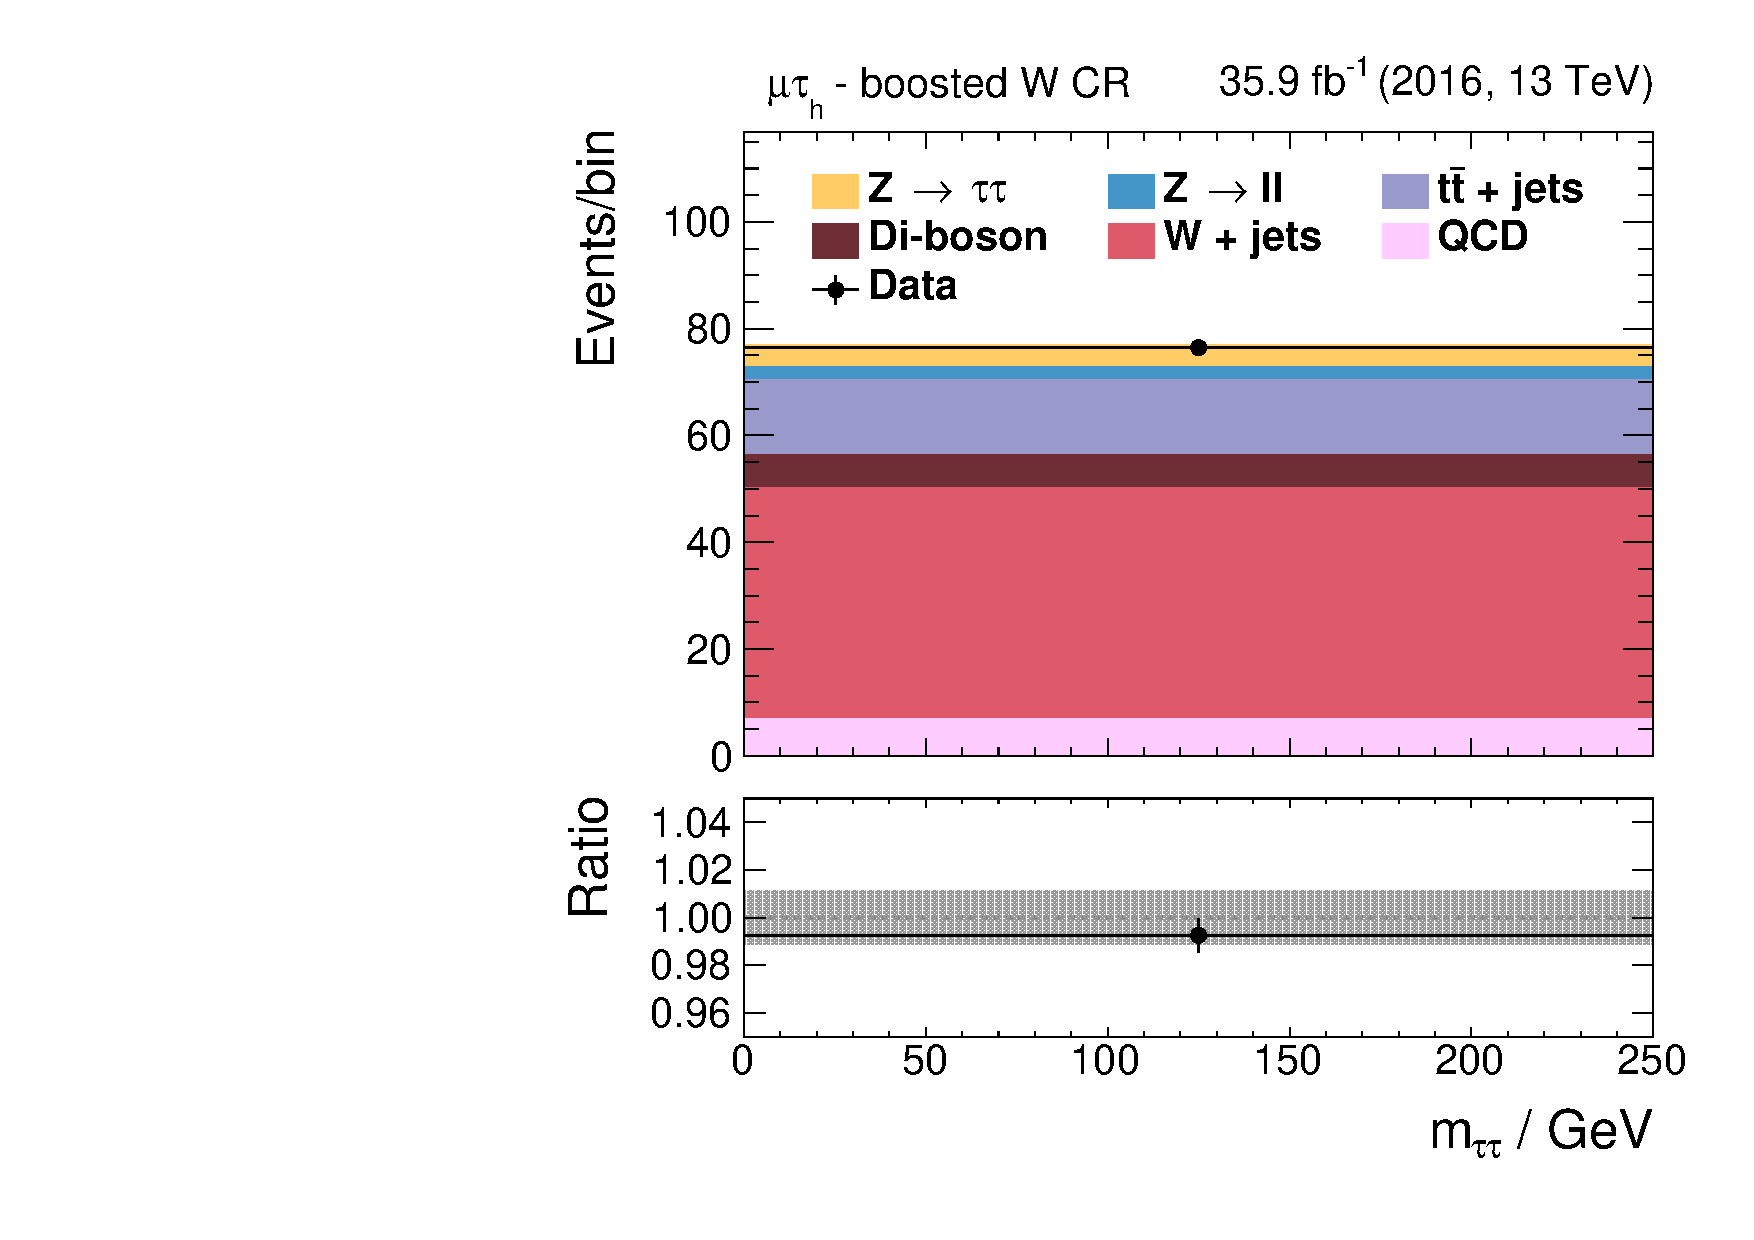
\includegraphics[width=0.47\textwidth]{Figures/background_estimation/qcd_mt_control-regions/htt_inputmt13__htt_mt_13_13TeV.pdf}
 \caption[\textit{Boosted} opposite-sign \textit{W+jets} control regions.]{Control region expected background normalization and data as given into the final fit for the W+jets OS high $m_\text{T}$ control region in the \textit{boosted} category for the $e\tau_\text{h}$ (left) and $\mu\tau_\text{h}$ (right) channel.}\label{fig:etmtqcd:0jet_w_ss_control}
\end{figure}

\clearpage

\subsection{QCD multijet background\label{sec:BackgroundEstimations:QCD}}

The contribution of QCD changes with for different decay channels as jets are likely to mimick hadronically decaying taus. As hadronization
is a complicated process, data-driven estimation techniques are utilized in all channels.

\subsubsection{$e\mu$ channel}

In the $e\mu$ channel the \textit{QCD} background is estimated in a sideband where the electric charges of electron and muon have the same sign.
As the QCD background is small in this channel, a customized background estimation has not been performed.
This means, the global OS/SS extrapolation factor measured for \cite{Sirunyan:2017khh} to be $R_\text{QCD}^\text{OS/SS}=2.22$ is used in all categories.
The SS QCD shape and yield is calculated by subtracting all other sources of backgrounds from SS data. The extrapolation factor is applied as a scale factor to get
the normalization in the signal region.

\subsubsection{$e\tau_\text{h}$ and $\mu\tau_\text{h}$ channels}

The \textit{QCD} background is estimated from events where the \tauh{} and the light lepton (e,$\mu$) have SS electric charges. The sideband is chosen such that it keeps all other selection criteria, that are applied in the 
signal region, fixed. To estimate the shape and the yield in the SS region, 
the small amounts of other backgrounds are subtracted from data. 
Except for \textit{W+jets}, that is modeled by the data-driven estimate obtained in section \ref{sec:BackgroundEstimations:W:etmt} with 
\begin{equation}
    N_\text{W}^\text{SS,SR} = R_\text{W}^\text{SS, high2low} \cdot N_\text{W}^\text{SS,CR},
\end{equation}
all other background contributions are taken from simulation. In order to obtain the final
QCD contribution 
\begin{equation}
    N_\text{QCD}^\text{OS,SR} = R_\text{QCD}^\text{OS/SS}\cdot N_\text{QCD}^\text{SS,SR}
\end{equation}
is used.
Here, $R_\text{QCD}^\text{OS/SS}$ is the QCD OS/SS extrapolation factor. 

\paragraph{QCD SS/OS extrapolation factor}\label{sec:qcdosss}\mbox{} \\ 
Studies of QCD Monte Carlo samples indicate that different fractions of SS and 
OS events in QCD backgrounds may be expected. For this reason, the ratio of SS to OS events must be measured to get a reliable 
QCD multijet background estimate in the signal region.
$R_\text{QCD}^\text{OS/SS}$ is determined in two sidebands orthogonal to the 
signal region  with inverted isolation of the light lepton. The factor measured in the \textit{near} sideband ($\text{0.1}<I_\text{rel}^\text{e}<\text{0.17}$ in $e\tau_\text{h}$ and $\text{0.15}<I_\text{rel}^{\mu}<\text{0.25}$ in $\mu\tau_\text{h}$)
is applied to SS events to estimate the final yield. This \textit{near} sideband ensures proximity to the signal region, but 
possesses a rather low purity in QCD events of roughly 30-50\%. % TODO: Check these numbers!
The measurement in the \textit{far} sideband ($\text{0.17}<I_\text{rel}^\text{e}<\text{0.5}$ in $e\tau_\text{h}$ and $\text{0.25}<I_\text{rel}^{\mu}<\text{0.5}$ in $\mu\tau_\text{h}$) is used to cross-check the measurement in the \textit{near} sideband
and to estimate the systematic uncertainty due to the assumption that the
measurement of the ratio in the \textit{near} sideband can be extrapolated to the 
signal region. Moreover, this region of phase space provides a significantly larger fraction of QCD events in the order of 80-90\%. % TODO: Check these numbers!
Since the fraction may strongly depend on the selection, $R_\text{QCD}^\text{OS/SS}$ is measured for each
signal category individually. In order to increase the event population in the two dijet categories, an inclusive selection of dijet events, omitting the $p_{\text{T}}^{\tau\tau}$ and the
$m_\text{jj}$ criteria, is chosen and the working point of the tau-ID is relaxed to \textit{very loose}. An exception of this procedure is made for the \textit{dijet lowboost} category in the $\mu\tau_\text{h}$ channel because the 
inclusive factor does not provide a reasonable data to MC agreement. There the same procedure as for the \textit{0-jet} and \textit{boosted} categories is applied. A summary of the exact selection criteria is given in table \ref{tab:backgroundEstimation:qcdossscategorization}.   

\begin{table}[h!]
    \caption[Selection criteria applied in the anti-isolated sideband for QCD OS/SS factor measurement.]{Selection criteria applied in the anti-isolated sidebands used to measure $R_\text{QCD}^\text{OS/SS}$. The factor is measured in the \textit{0-jet}, \textit{boosted} and an inclusive \textit{dijet} category for the two dijet signal categories. An exception is made for the \textit{dijet lowboost} signal category in the $\mu\tau_\text{h}$ channel, in which the inclusive scale factor did not
provide a good agreement between data and MC.}\label{tab:backgroundEstimation:qcdossscategorization}
    \begin{tabular}{clcc}
        \toprule
         Name & Category  & Near & Far   \\ \hline
        \multirow{2}{*}{{\small 0-jet}} & \multirow{2}{*}{{\small No jet, b-tag veto}} & \multirow{4}{*}{{\small$\text{0.1}<I_\text{rel}^\text{e}<\text{0.17}$ in $e\tau_\text{h}$}} & \multirow{4}{*}{{\small$\text{0.17}<I_\text{rel}^\text{e}<\text{0.5}$ in $e\tau_\text{h}$}}  \\
                              &                                         &                                                          &     \\ \cline{1-2}
        \multirow{2}{*}{{\small boosted}} & {\small (!0-jet, !dijet)    }                  &                                                          &          \\
                              &          {\small $\|$(One jet, b-tag veto) } & \\ \cline{1-2}
        \multirow{2}{*}{{\small dijet}} & {\small \geq 1 jet, b-tag veto,   }              &   \multirow{4}{*}{{\small$\text{0.15}<I_\text{rel}^{\mu}<\text{0.25}$ in $\mu\tau_\text{h}$}}& \multirow{4}{*}{{\small$\text{0.25}<I_\text{rel}^{\mu}<\text{0.5}$ in $\mu\tau_\text{h}$}}         \\
                              &  {\small $\tau_\text{h}$ WP VLoose Isolation  }   &      & \\ \cline{1-2}
        \multirow{2}{*}{{\small $\mu\tau_\text{h}$ lowboost}} & {\small \geq 1 jet,$p^{\tau\tau}_\text{T}<\text{200\,GeV}$,}                     &                                        \\
                              &  {\small b-tag veto, $m_\text{jj}>\text{300\,GeV}$ }      &  \\                              

		\bottomrule
    \end{tabular}
\end{table}

The extrapolation factor is determined performing a binned maximum-likelihood fit to the visible mass distribution in OS events treating QCD as signal process. 
As a first estimate for QCD in the respective OS sideband, $N_\text{QCD}^\text{OS,prefit}$, the QCD contribution from SS events is taken which is calculated subtracting all sources of simulated backgrounds (in this sideband also \textit{W+jets}) from SS data
\begin{equation}
    N_\text{QCD}^\text{OS,prefit} = N_\text{QCD}^\text{SS} = N_\text{data}^\text{SS} - \sum_{i \in \{ZTT,ZLL,TT,VV,W,qqH \}} N_{i}^\text{SS}.
\end{equation}
This is equivalent to choosing $R_\text{QCD}^\text{OS/SS} = 1$. During the fit all backgrounds are allowed to float within their uncertainties. Therefore, normalization 
uncertainties for all backgrounds that are subtracted from data; an uncertainty on the luminosity 
of $\text{2.5\%}$; trigger efficiency uncertainties for tau leptons ($\text{3\%}$), muons ($\text{2\%}$) and 
electrons ($\text{2\%}$); the $e\rightarrow \tau$ misidentification rate uncertainty of $\text{12\%}$; the $\mathsf{\mu \rightarrow \tau}$
misidentification rate uncertainty of $\text{ 25\%}$ and the decay-mode specific tau energy scale shape uncertainty are taken into account.

The QCD signal strength modifier $r_\text{QCD}$ after performing the fit in the \textit{near} sideband is subsequently taken as the QCD OS/SS factor. 
This factor is read off from the profile likelihood function for $r_\text{QCD}$  as examplary shown for the \textit{boosted} category in the $\mu\tau_\text{h}$
channel for both \textit{near} and \textit{far} sidebands in \figreft{BK:Scans:mt_boosted}. More fit result are found in the appendix in section \ref{suppsec:fits}.
\begin{figure}
    \centering
    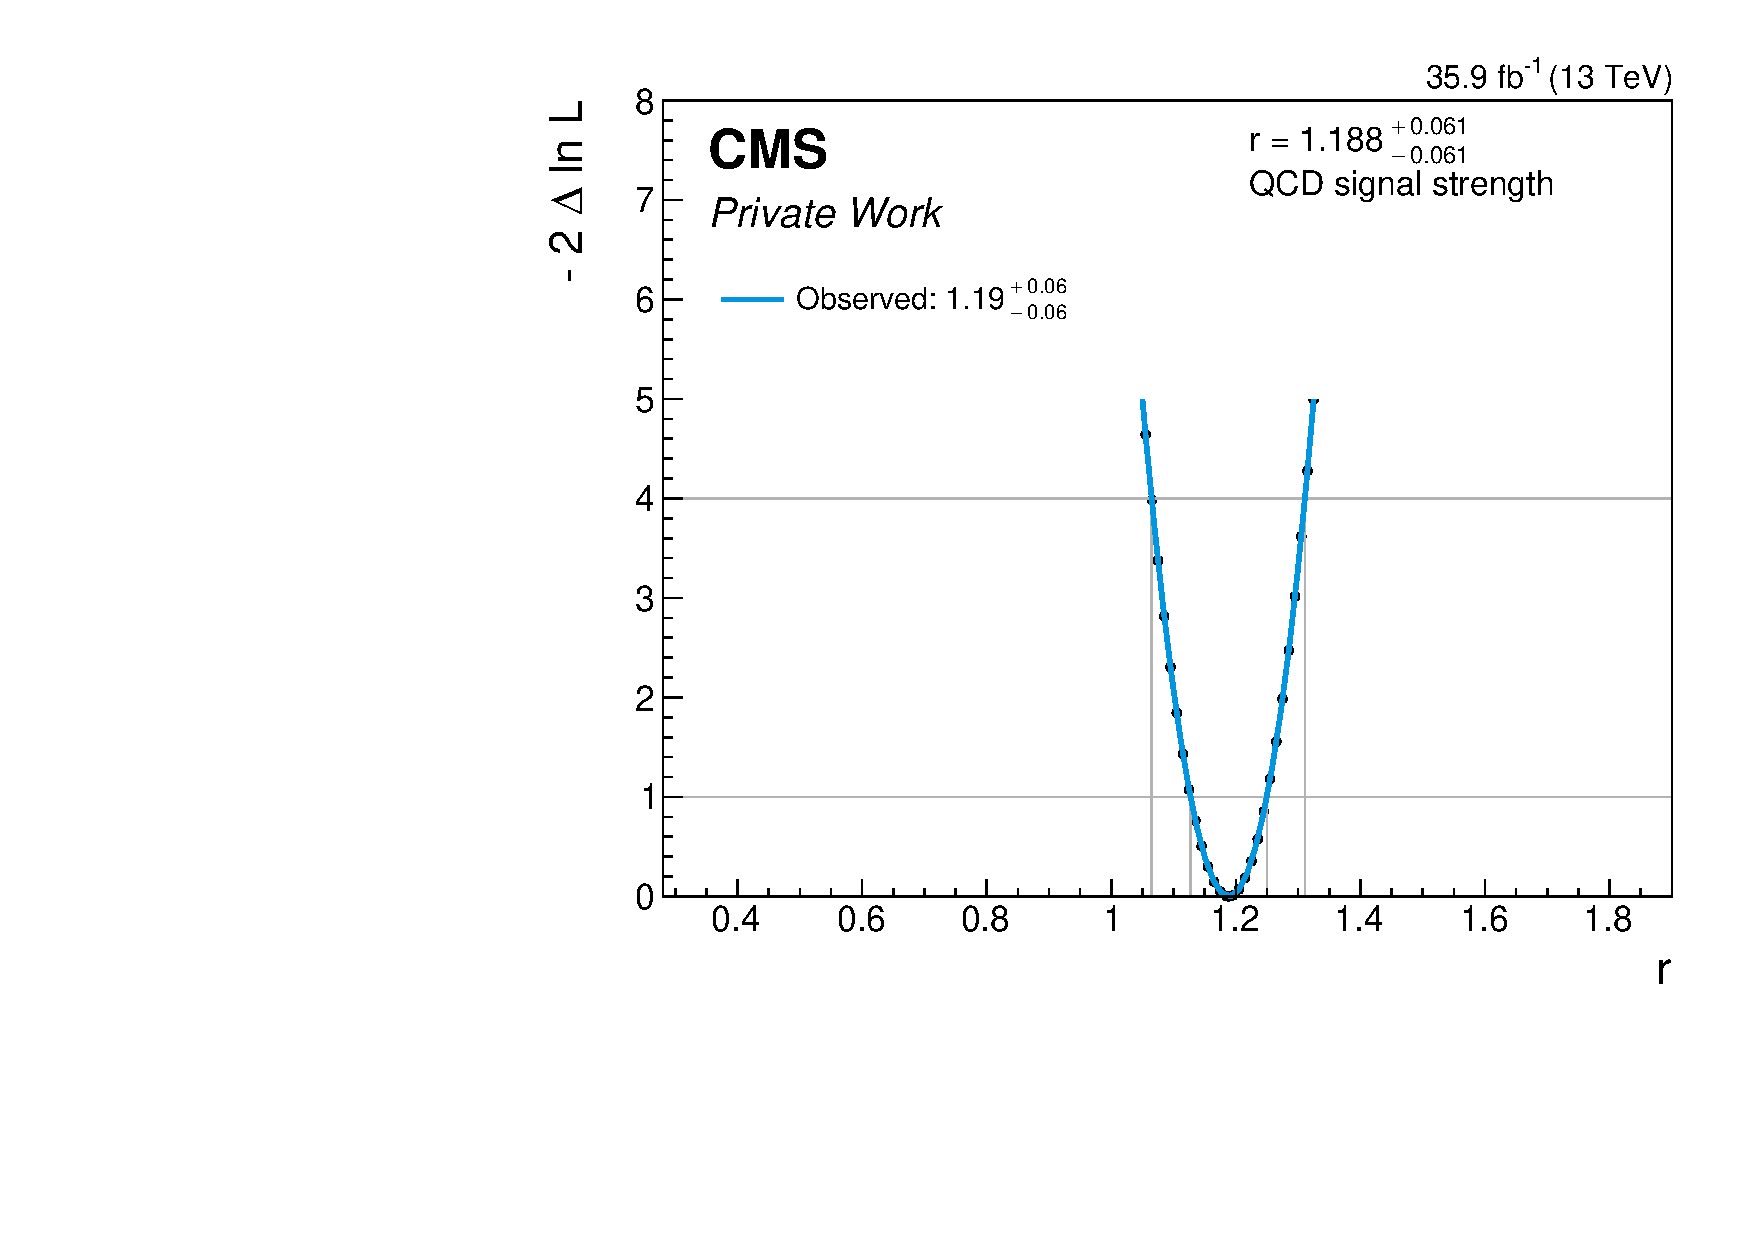
\includegraphics[width=.49\textwidth]{Figures/background_estimation/RQCDOSSS/Scans/mt_Boosted2D_antiiso_near/plots/nll.pdf}
    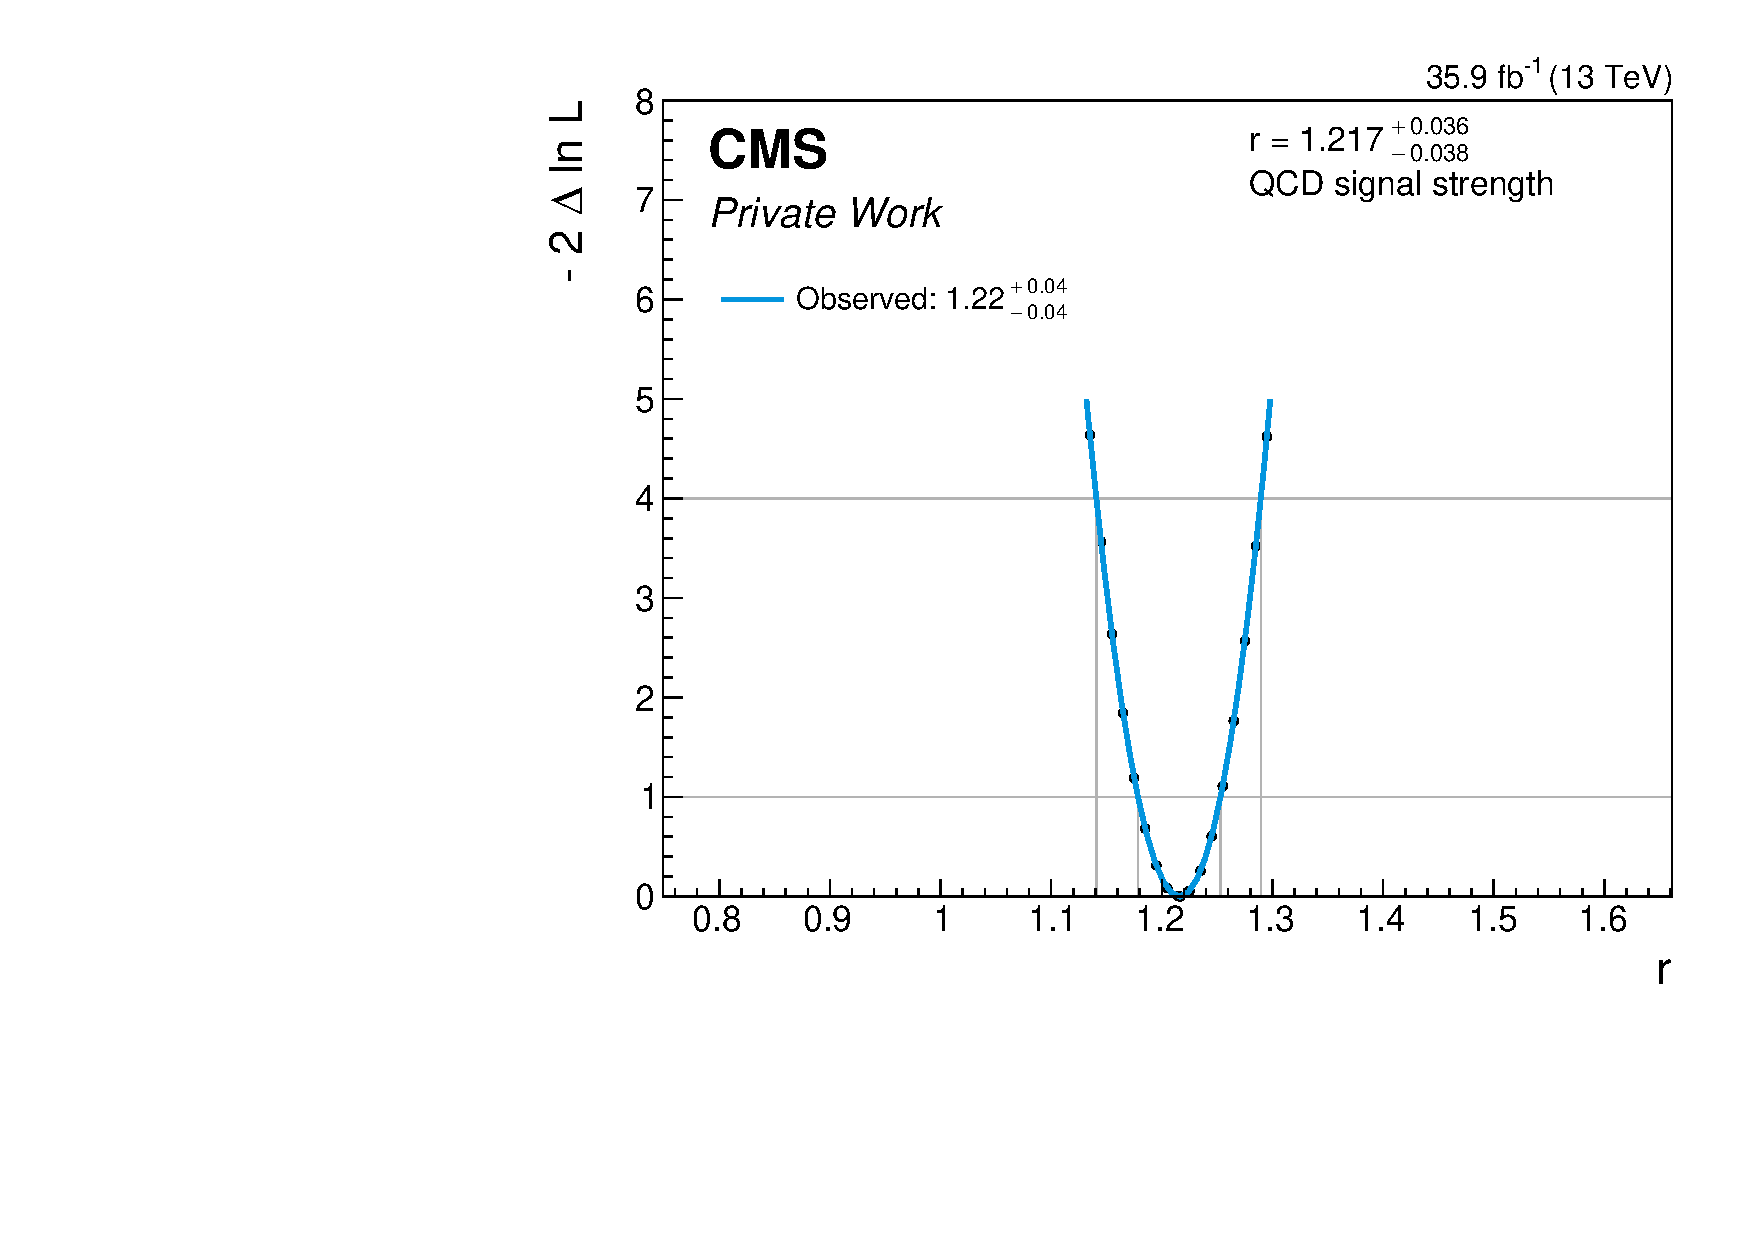
\includegraphics[width=.49\textwidth]{Figures/background_estimation/RQCDOSSS/Scans/mt_Boosted2D_antiiso_far/plots/nll.pdf}
    \caption[Max. likelihood fit results of the $r_\text{QCD}$ in the in the $\mu\tau_\text{h}$ channel in the \textit{boosted} category.]{Results of the maximum likelihood scan to find the signal strength of the QCD multijet background in the $\mu\tau_\text{h}$ channel in the \textit{boosted} category.
    The signal strength parameter from the near sideband (left figure) $r^{\text{near}}_\text{QCD} = \text{1.19\pm 0.6}$ is taken as the QCD OS/SS factor. As statistical uncertainty the larger value of the two given thresholds is chosen. 
    $r^{\text{near}}_\text{QCD}$ is compared to the value $r^{\text{far}}_\text{QCD} = \text{1.22\pm 0.04}$ obtained in the \textit{far} sideband (right plot). As they agree within their uncertainties the statistical uncertainties of the far sideband is assigned as systematic extrapolation uncertainty.}\label{BK:Scans:mt_boosted}
\end{figure}

The uncertainty given by the fit is added as a systematic uncertainty. Furthermore, an uncertainty $\sigma_{\text{QCD-Extrap}}$, covering the extrapolation from the \textit{near} sideband to the signal
region, is estimated comparing the measured factors in the \textit{near} and the \textit{far} sideband and added to the fit uncertainty of the \textit{near} measurement. 
If both factors agree within their uncertainties, the extrapolation uncertainty is covered by the fit uncertainty in the \textit{far} sideband
\begin{equation}
    \sigma_{\text{QCD-Extrap}} =  \sigma_{\text{far}}.
\end{equation}
If they do not agree, the difference between the two measured factors
\begin{equation}
    \sigma_{\text{QCD-Extrap}} =  \abs{R_{\text{QCD, near}}^\text{OS/SS} - R_{\text{QCD, far}}^\text{OS/SS} }
\end{equation}
is taken.
The quadratic sum $\sigma_\text{QCD}^\text{tot}$ of the near fit uncertainty and the  extrapolation uncertainty is given as a single systematic uncertainty to the final fit.
The results of the QCD OS/SS factor measurements are stated in table \ref{tab:backgroundEstimation:qcdosss_result_0jet}.
Examples for the outcome of the fits in the \textit{near} and \textit{far} sidebands are given in \figreft{BK:Scans:mt_boosted}.
The expected background modeling and data before (Prefit) and after the likelihood fit (Postfit) for each category in the \textit{near} sideband is shown in figures \ref{fig:etmtqcd:et_prefitpostfit_near} and \ref{fig:etmtqcd:mt_prefitpostfit_near}. Additionally, the distributions in the \mutau{} channel in the \textit{dijet lowboost} category can be found
in figure \ref{fig:etmtqcd:mt_prefitpostfit_lowboost_near}.
% Measurement in the 0jet category
\begin{table}[h]
    \centering
    \caption[Measured QCD OS/SS extrapolation factors and systematic uncertainties.]{Measured QCD OS/SS extrapolation factors and systematic uncertainties in the \textit{0-jet}, \textit{boosted} and \textit{dijet} categories. Furthermore, an individual factor is measured for the \textit{dijet lowboost} category in the
    $\mu\tau_\text{h}$ channel, because the inclusively measured factor does not provide a good data to MC agreement.
    The best-fit signal strength modifier value and the uncertainty read off from the profile likelihood function are given and the relative uncertainty stated in brackets.
    The total uncertainty is calculated from the quadratic sum of the uncertainties from the \textit{near} fit and the extrapolation uncertainty given by the \textit{far} fit uncertainty or the difference of the
    \textit{near} and \textit{far} measurements.} \label{tab:backgroundEstimation:qcdosss_result_0jet}
    \begin{tabular}{ccccc}
        \toprule
         Category              & Channel    & $r_\text{QCD}^\text{near}\text{(\pm rel.unc[\%])}$ & $r_\text{QCD}^\text{far}\text{(\pm rel.unc[\%])}$&      $\sigma_\text{QCD}^\text{tot}[\%]$  \\ \hline
        \multirow{2}{*}{0-jet} & $e\tau_\text{h}$   &           $\text{1.20 \pm 0.08}$ (7.6)     & $\text{0.98 \pm 0.07}$ (7.1)  & 14.8        \\
                               & $\mu\tau_\text{h}$ &           $\text{1.15 \pm 0.04}$ (3.4)     & $\text{1.25 \pm 0.02}$ (1.6)  & 9.3       \\
        \multirow{2}{*}{boosted} & $e\tau_\text{h}$ &           $\text{1.76 \pm 0.22}$ (12.5)    & $\text{1.11 \pm 0.12}$ (11)   & 38      \\
                               & $\mu\tau_\text{h}$ &           $\text{1.19 \pm 0.06}$ (5.0)     & $\text{1.18 \pm 0.04}$ (3.3)  & 6     \\
        \multirow{2}{*}{dijet (inclusive)} & $e\tau_\text{h}$ & $\text{2.00 \pm 0.27}$ (13.5)    & $\text{1.02 \pm 0.09}$ (8.8)  &  47      \\
                               & $\mu\tau_\text{h}$ &           $\text{1.30 \pm 0.06}$ (4.6)     & $\text{1.13 \pm 0.06}$ (5.3)  & 11     \\ \midrule
        \multirow{1}{*}{dijet lowboost} & $\mu\tau_\text{h}$ &  $\text{1.60 \pm 0.31}$ (19.3)    & $\text{1.42 \pm 0.20}$ (14)   & 23      \\ \bottomrule
    \end{tabular}%
\end{table}% 

\begin{figure}[h!]
    \centering
    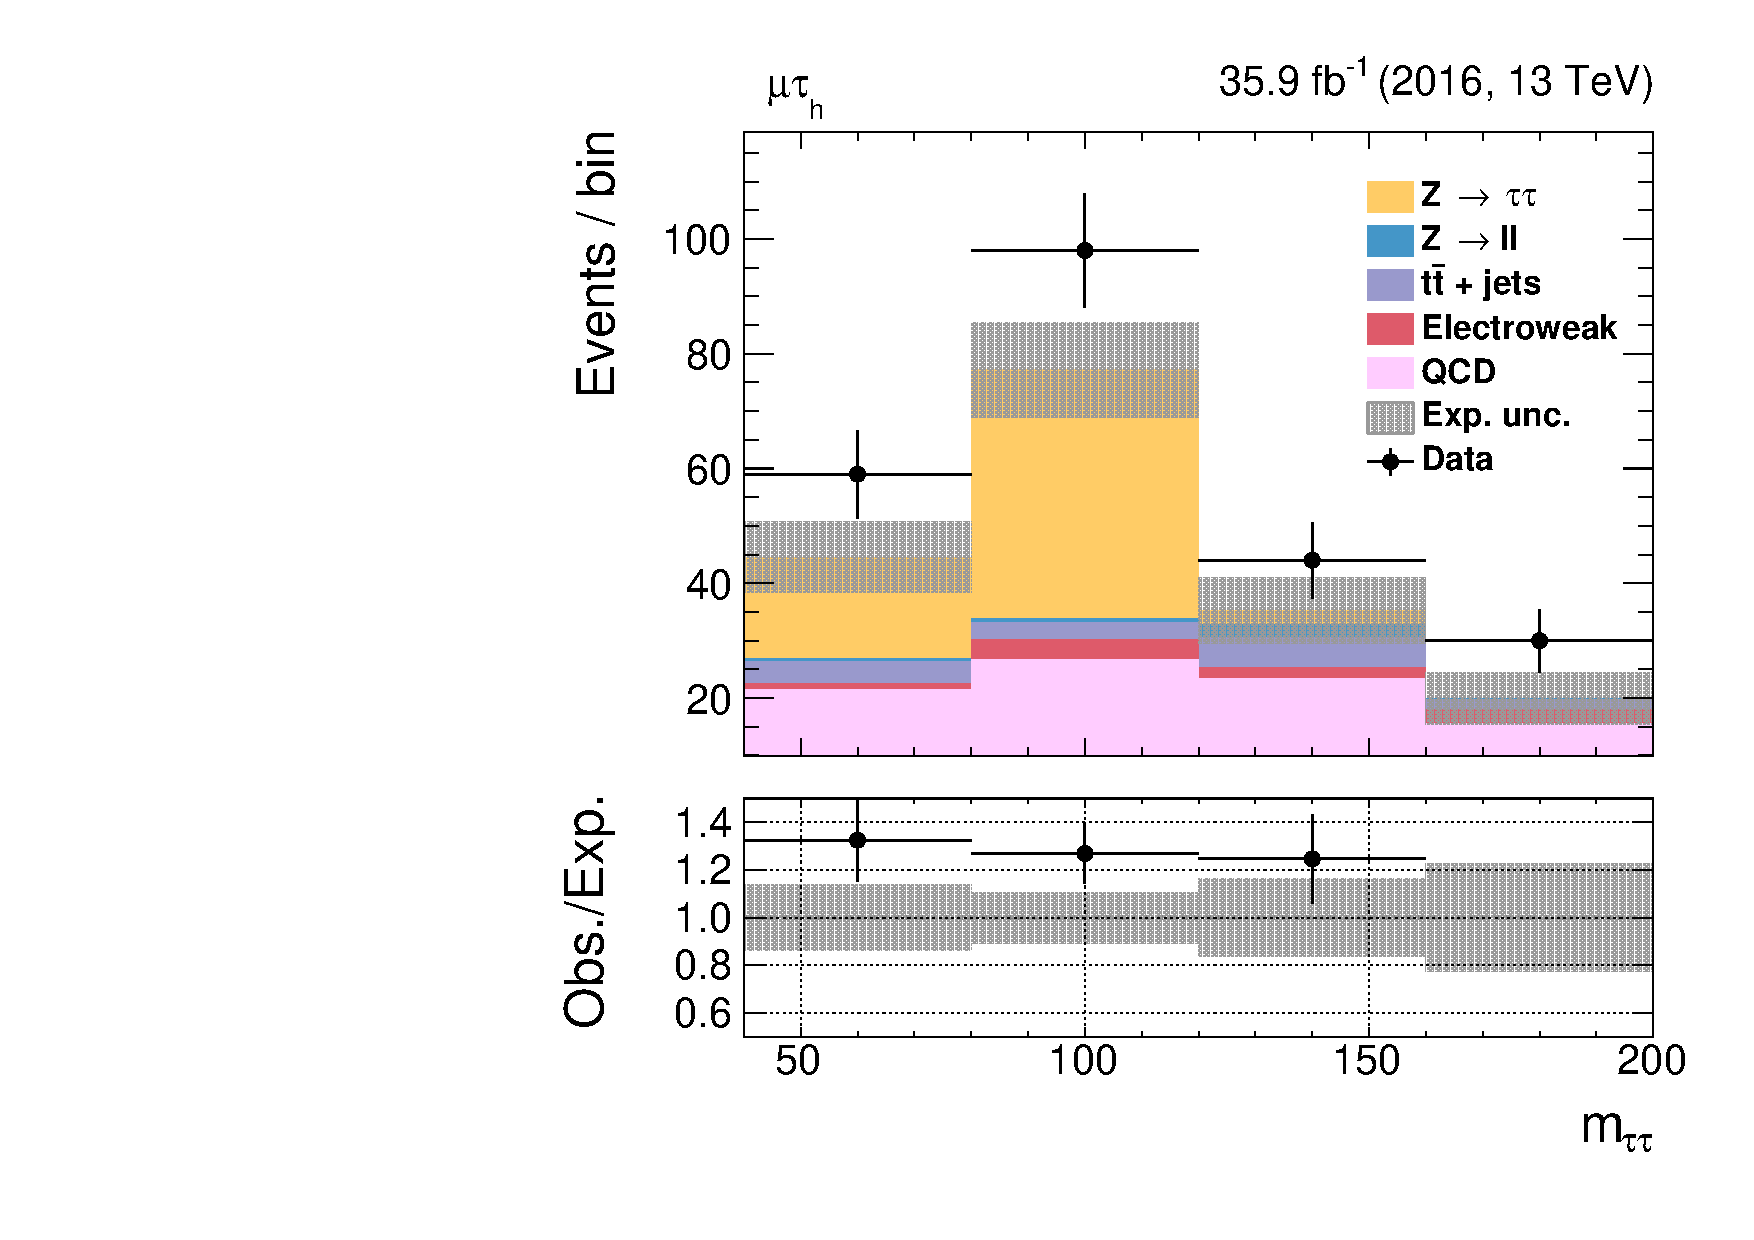
\includegraphics[width=0.47\textwidth]{Figures/background_estimation/RQCDOSSS/Postfit/mt_dijet2D_lowboost_antiiso_near/prefit_mt_dijet2D_lowboost_antiiso_near.pdf}
    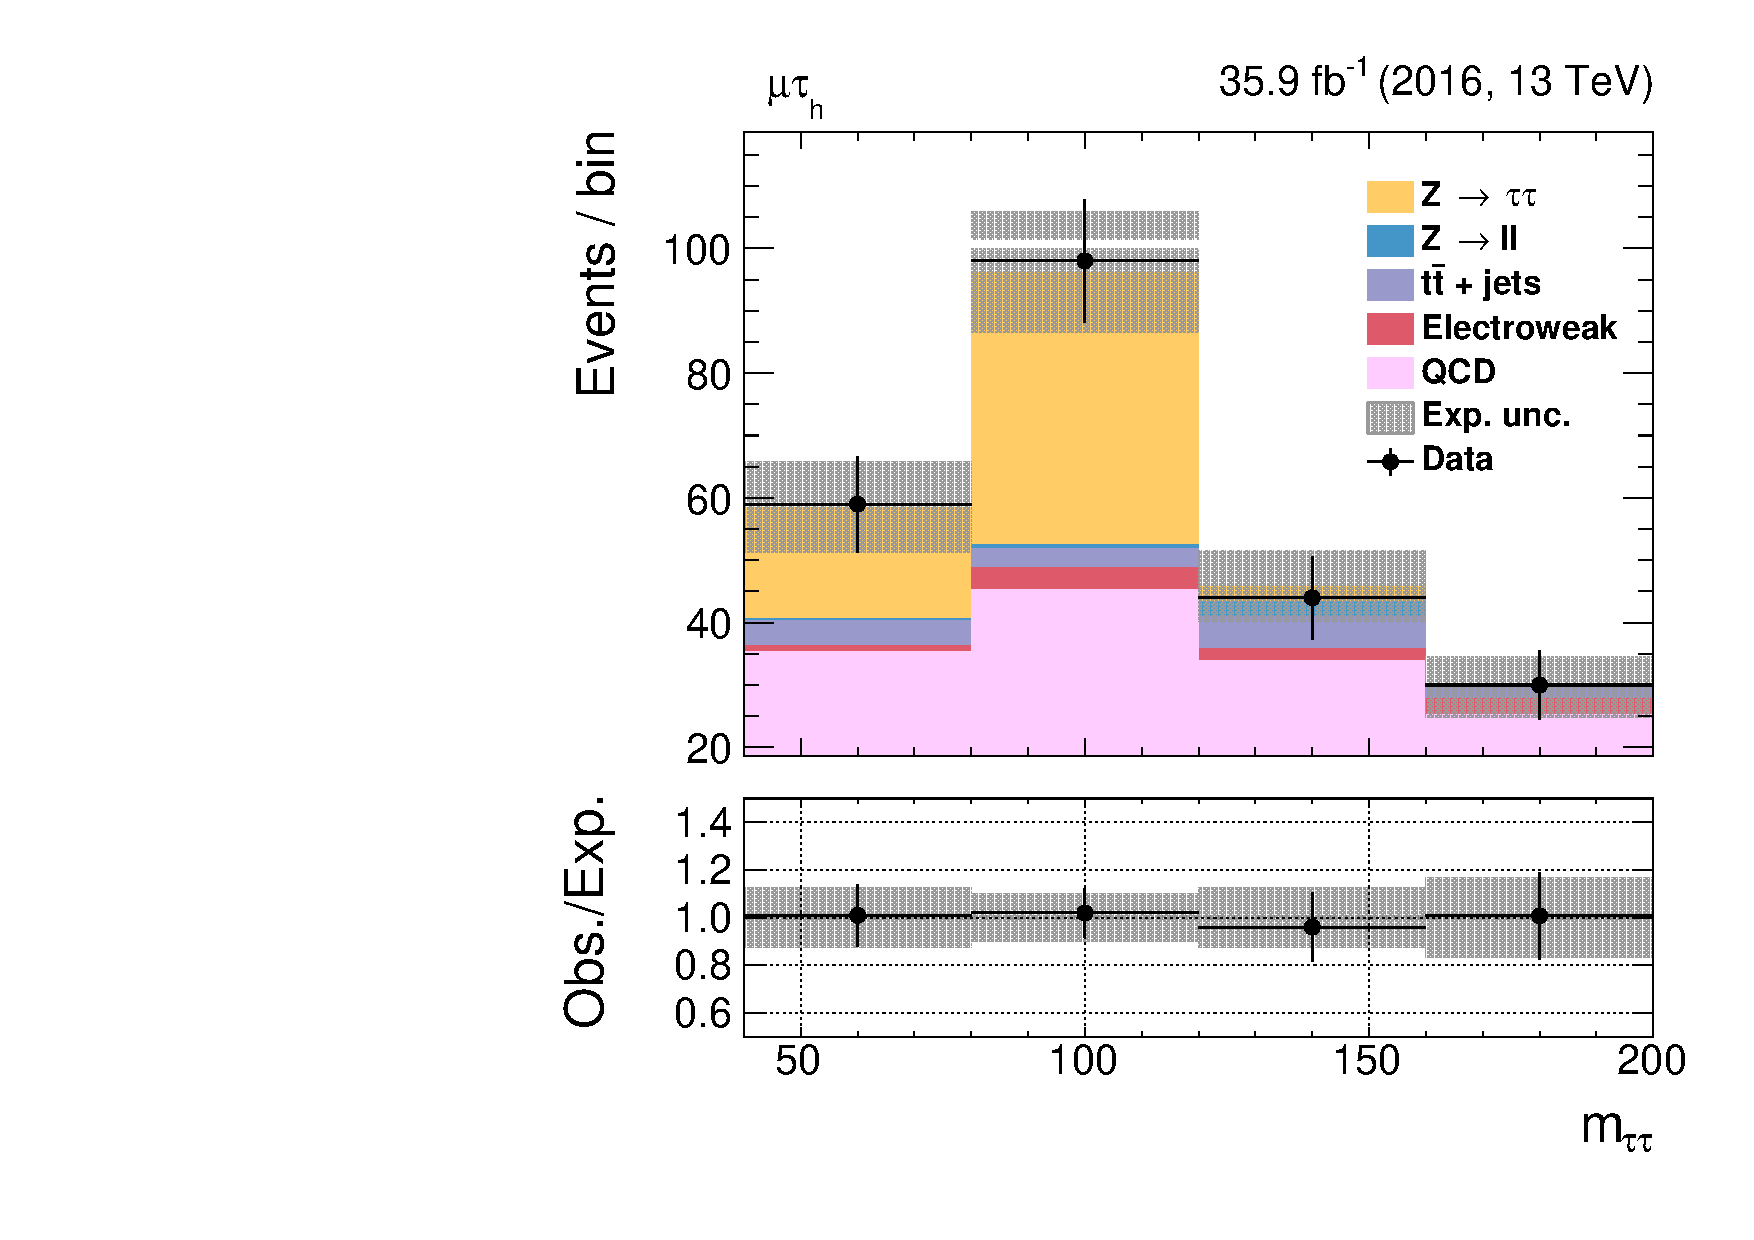
\includegraphics[width=0.47\textwidth]{Figures/background_estimation/RQCDOSSS/Postfit/mt_dijet2D_lowboost_antiiso_near/postfit_mt_dijet2D_lowboost_antiiso_near.pdf}
     \caption[Prefit and Postfit distributions in the $\mu\tau_\text{h}$ channel for the \textit{near} sideband in the \textit{dijet lowboost} category.]{Prefit and postfit distributions in the $\mu\tau_\text{h}$ channel and the \textit{dijet lowboost} category for the \textit{near} sideband.}\label{fig:etmtqcd:mt_prefitpostfit_lowboost_near}
\end{figure}%
% python HiggsAnalysis/KITHiggsToTauTau/scripts/makePlots_datacardsQCDfactors.py -i /nfs/dust/cms/user/dwolfsch/htautau/artus/2018-08-07_18-44_Run2CPStudies_Nominal_Summer16_plusHToTauTauM110-140/merged/ -c et -c mt --categories ZeroJet2D_antiiso_near Boosted2D_antiiso_near dijet2D_lowboost_antiiso_near dijet2D_antiiso_near --www background_studies/near_20180925 --log-level debug -o /afs/desy.de/user/d/dwolfsch/cms_analysis/CMSSW_8_1_0/src/plots/QcdFactorsStudies_datacards/near_20180925 
% python HiggsAnalysis/KITHiggsToTauTau/scripts/makePlots_datacardsQCDfactors.py -i /nfs/dust/cms/user/dwolfsch/htautau/artus/2018-08-07_18-44_Run2CPStudies_Nominal_Summer16_plusHToTauTauM110-140/merged/ -c et -c mt --categories ZeroJet2D_antiiso_far Boosted2D_antiiso_far dijet2D_lowboost_antiiso_far dijet2D_antiiso_far --www background_studies/far_20180925 --log-level debug -o /afs/desy.de/user/d/dwolfsch/cms_analysis/CMSSW_8_1_0/src/plots/QcdFactorsStudies_datacards/far_20180925 
\begin{figure}[h]
    \centering
  {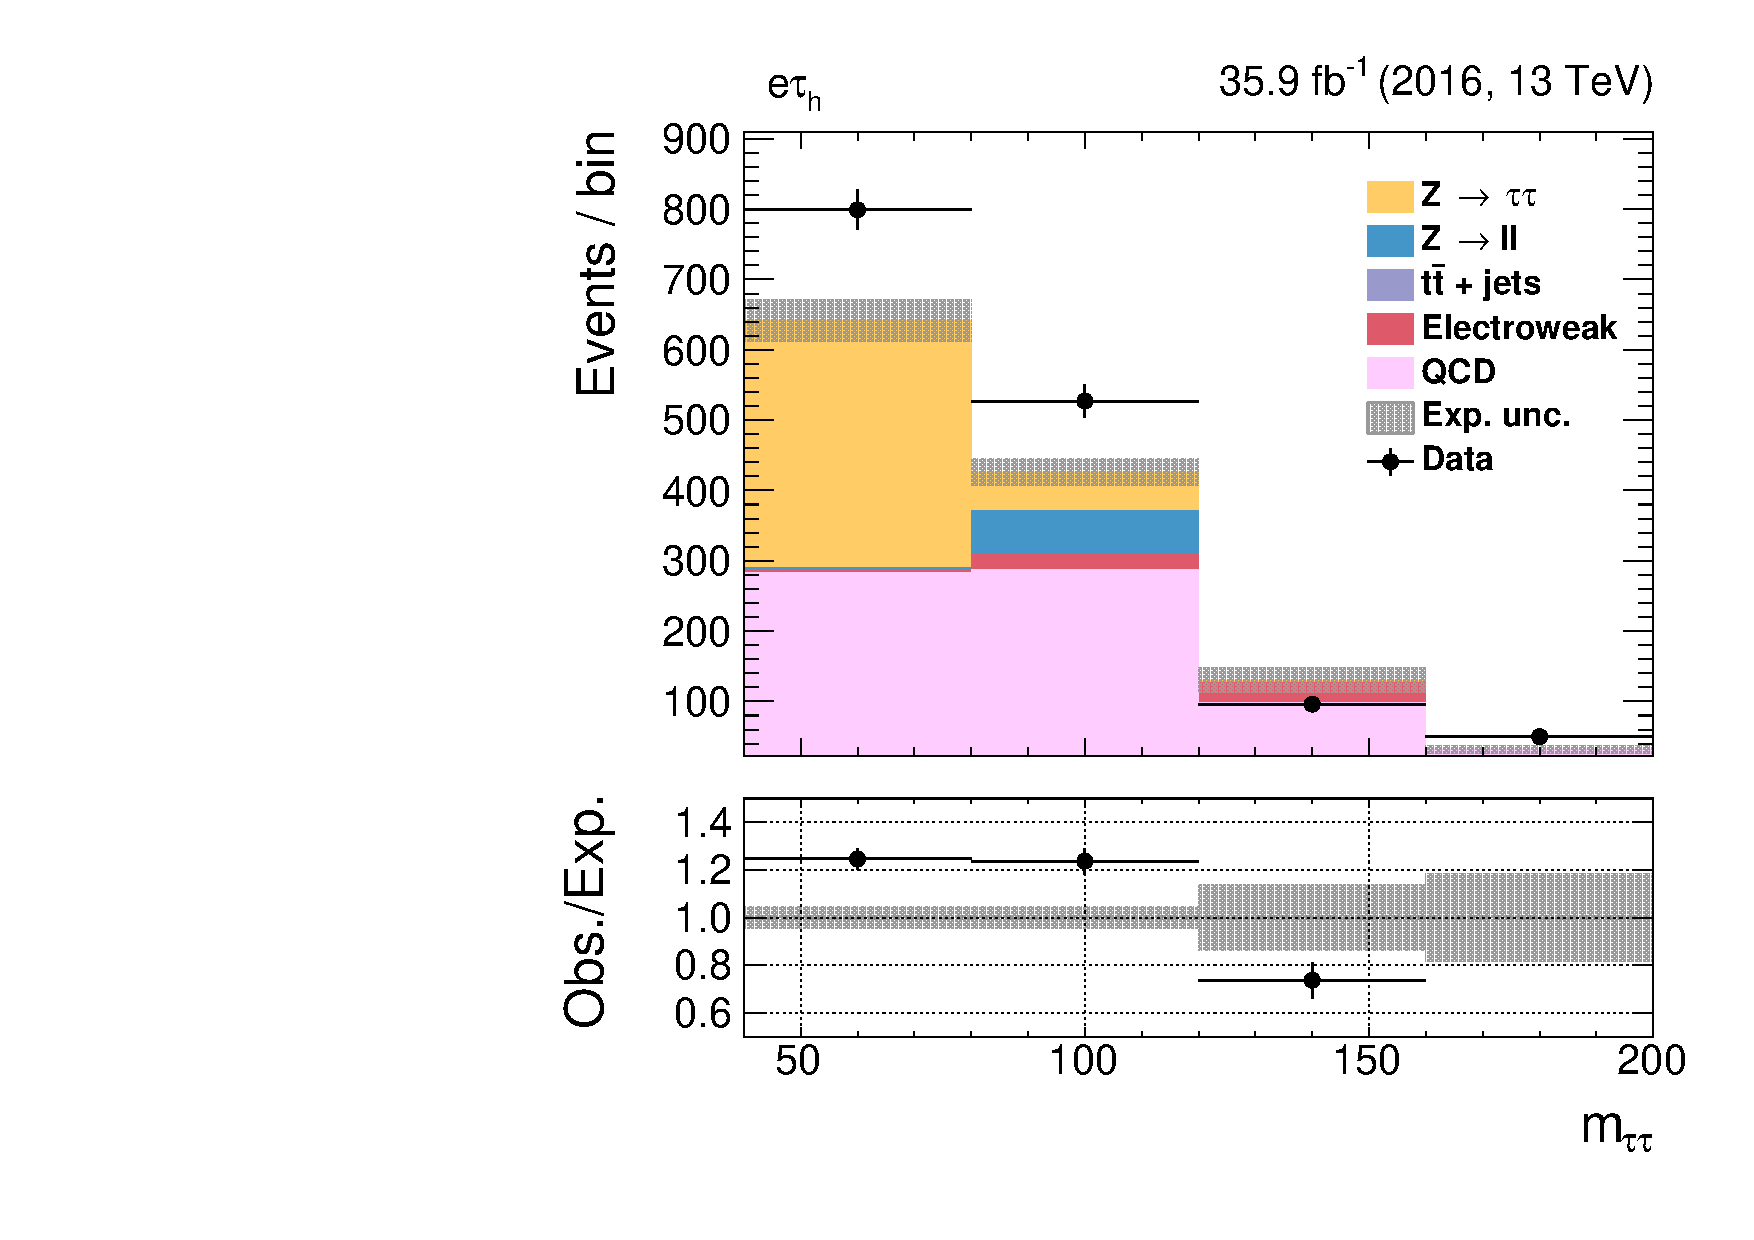
\includegraphics[width=0.47\textwidth]{Figures/background_estimation/RQCDOSSS/Postfit/et_ZeroJet2D_antiiso_near/prefit_et_ZeroJet2D_antiiso_near.pdf}}
  {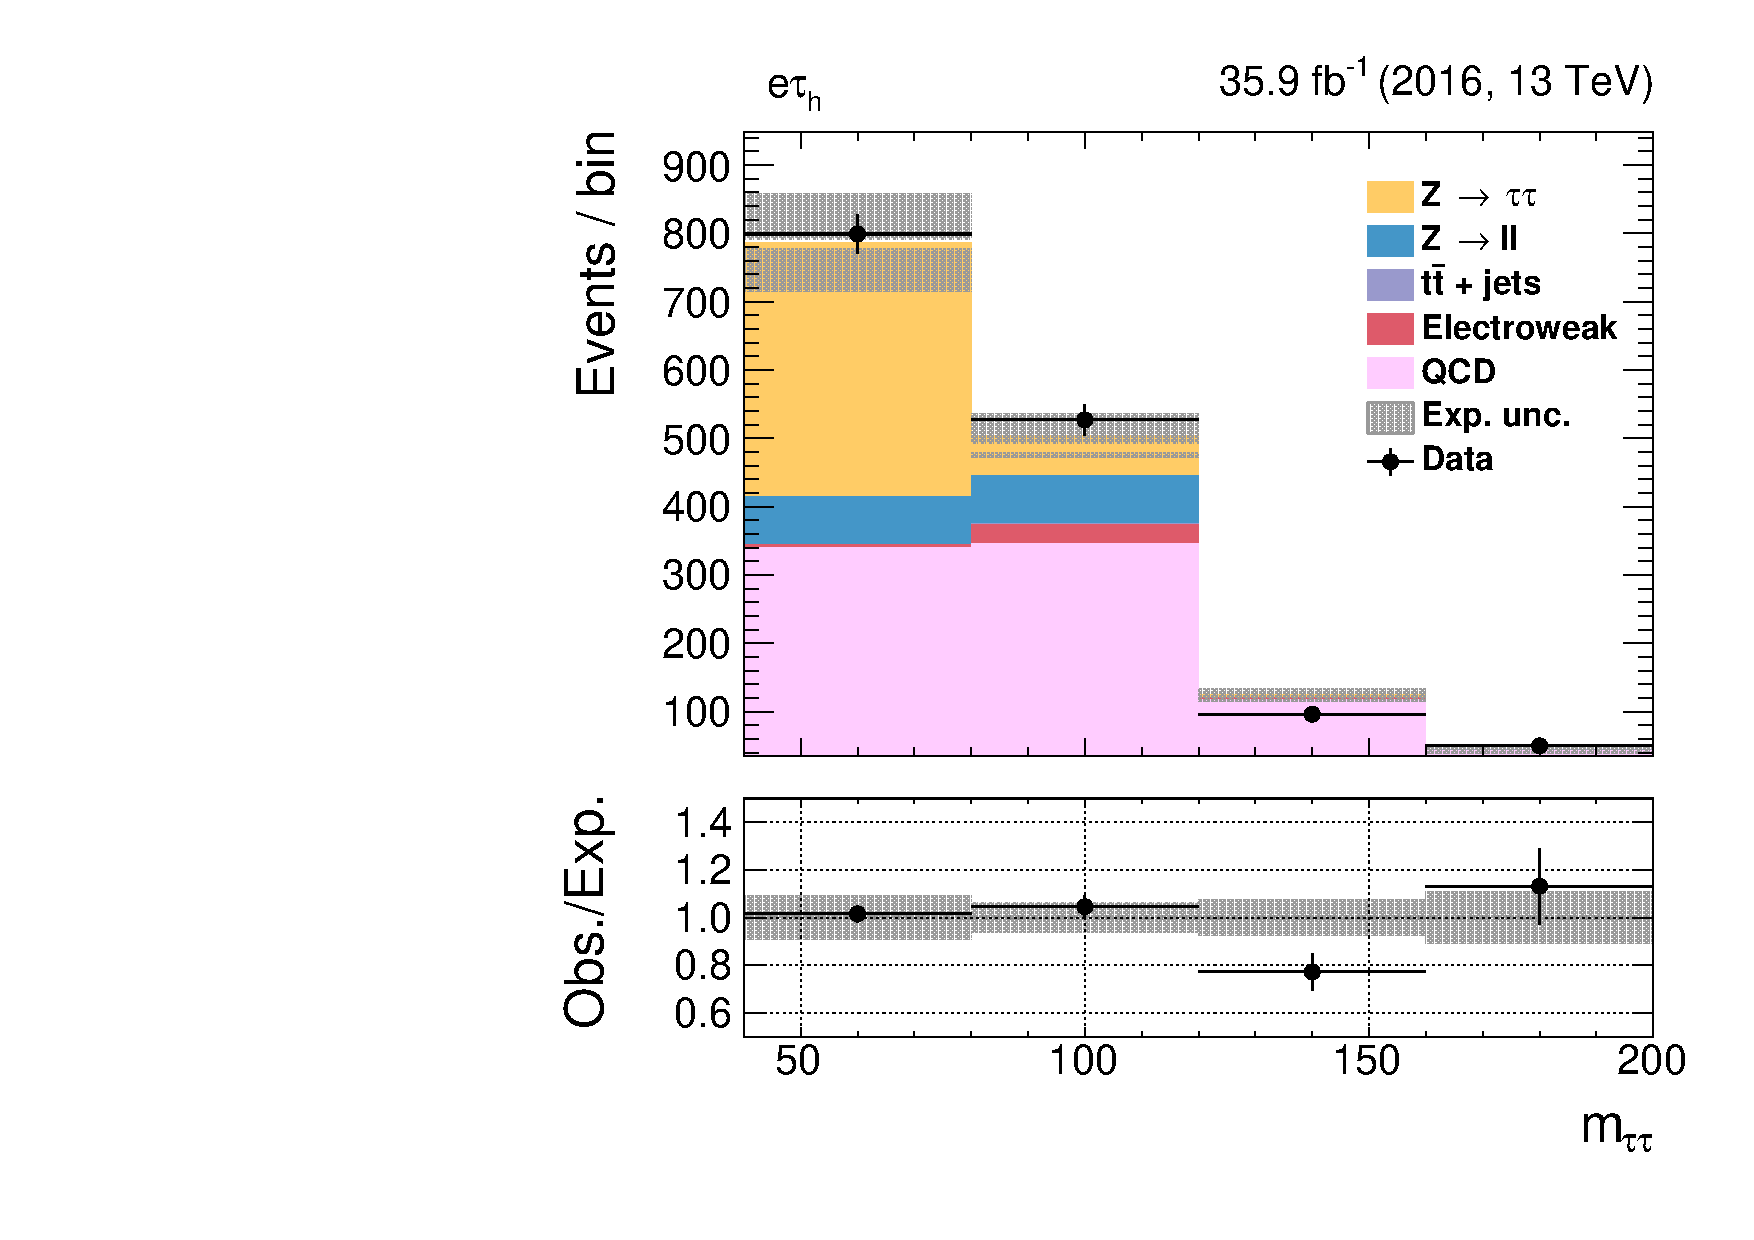
\includegraphics[width=0.47\textwidth]{Figures/background_estimation/RQCDOSSS/Postfit/et_ZeroJet2D_antiiso_near/postfit_et_ZeroJet2D_antiiso_near.pdf}} \\ 
  {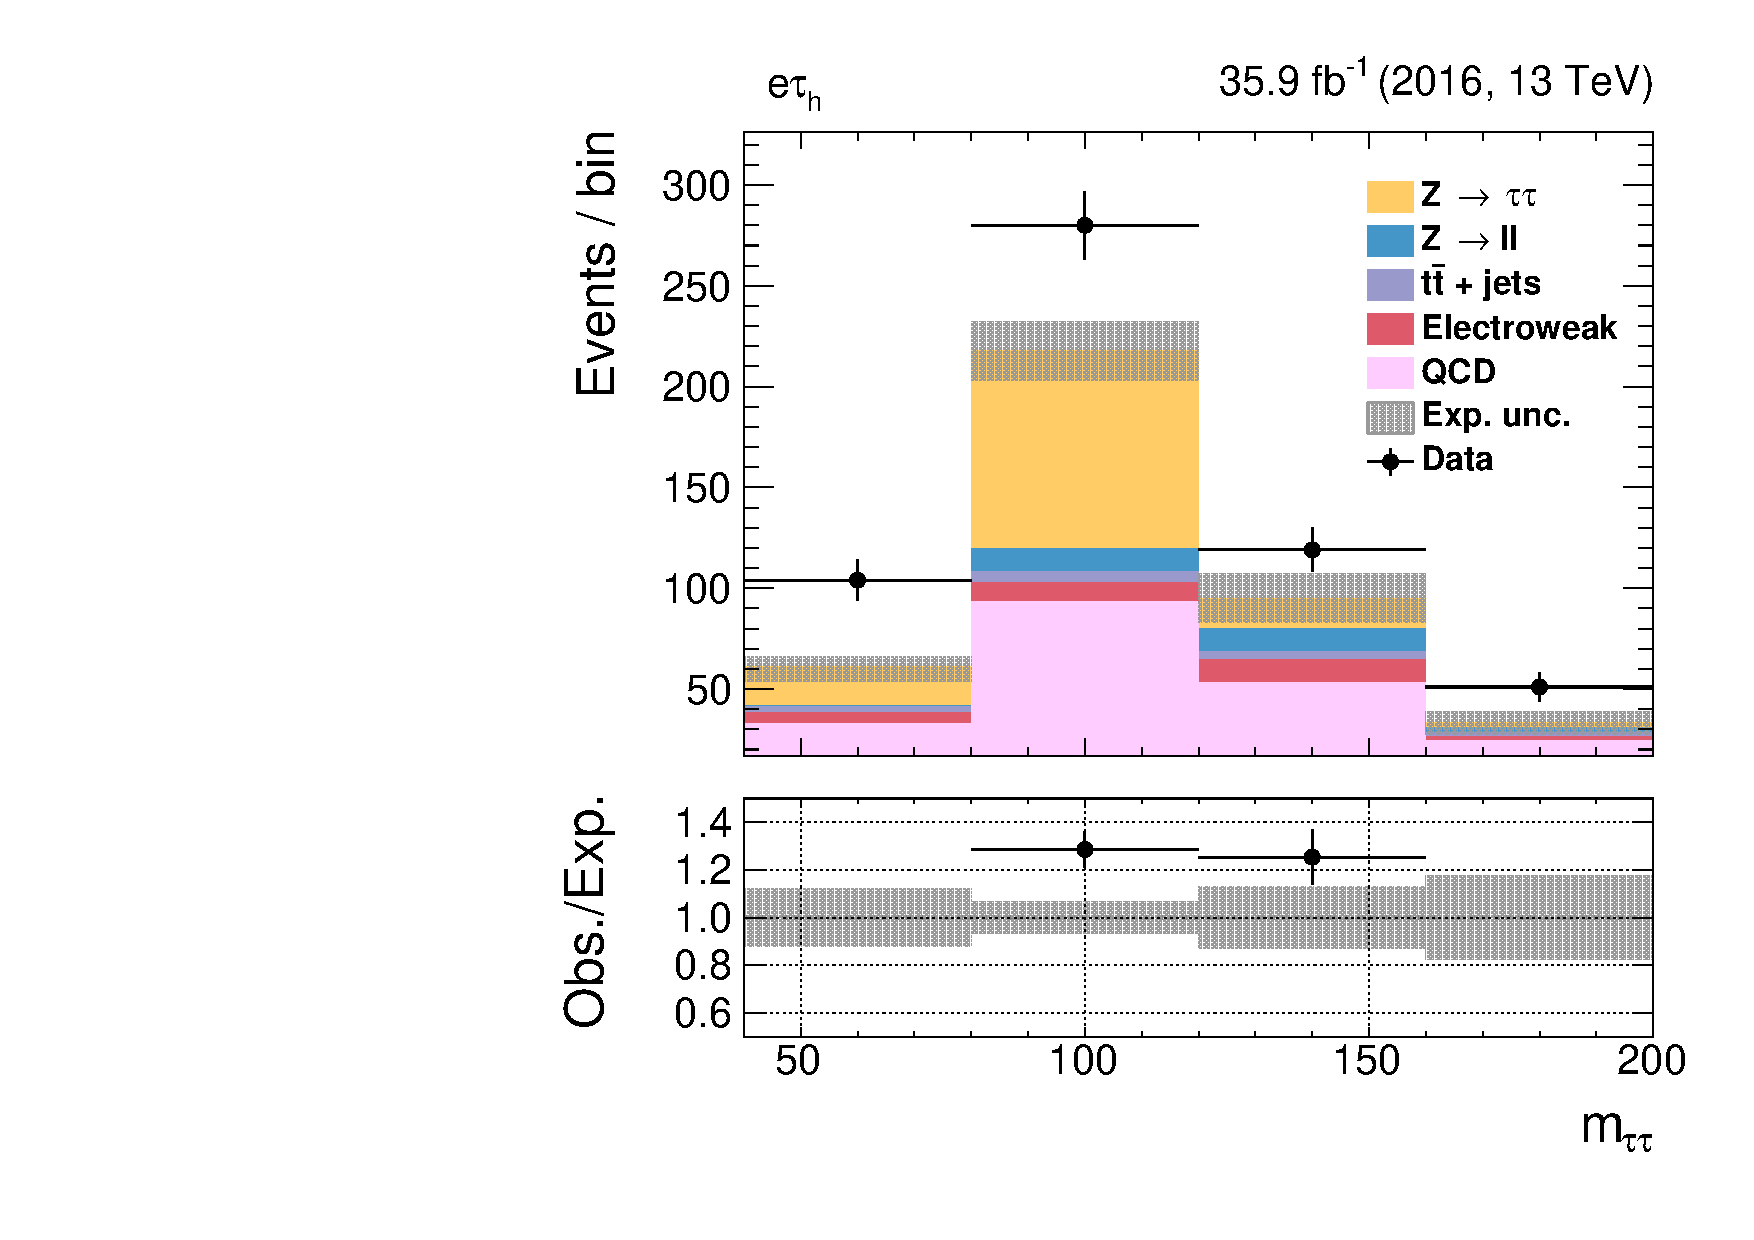
\includegraphics[width=0.47\textwidth]{Figures/background_estimation/RQCDOSSS/Postfit/et_Boosted2D_antiiso_near/prefit_et_Boosted2D_antiiso_near.pdf}}
  {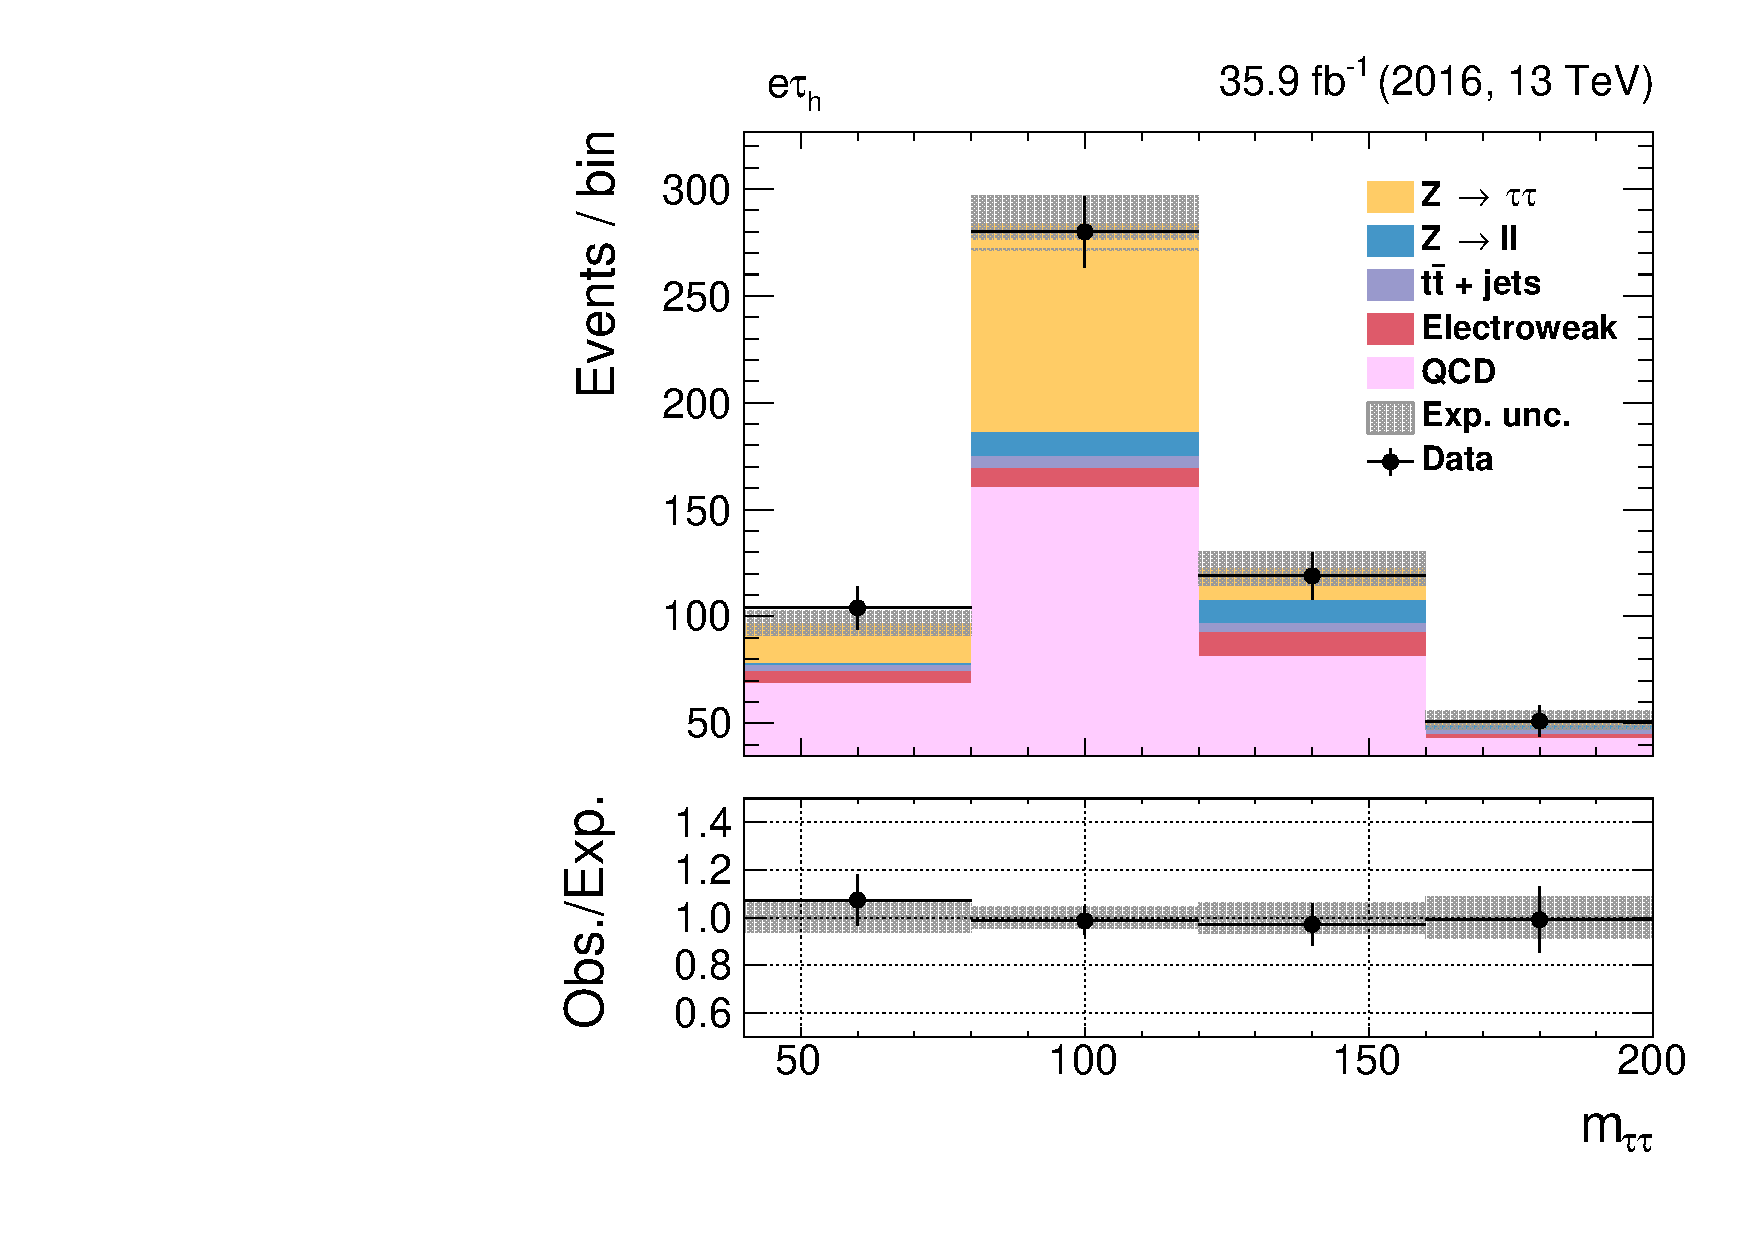
\includegraphics[width=0.47\textwidth]{Figures/background_estimation/RQCDOSSS/Postfit/et_Boosted2D_antiiso_near/postfit_et_Boosted2D_antiiso_near.pdf}} \\
  {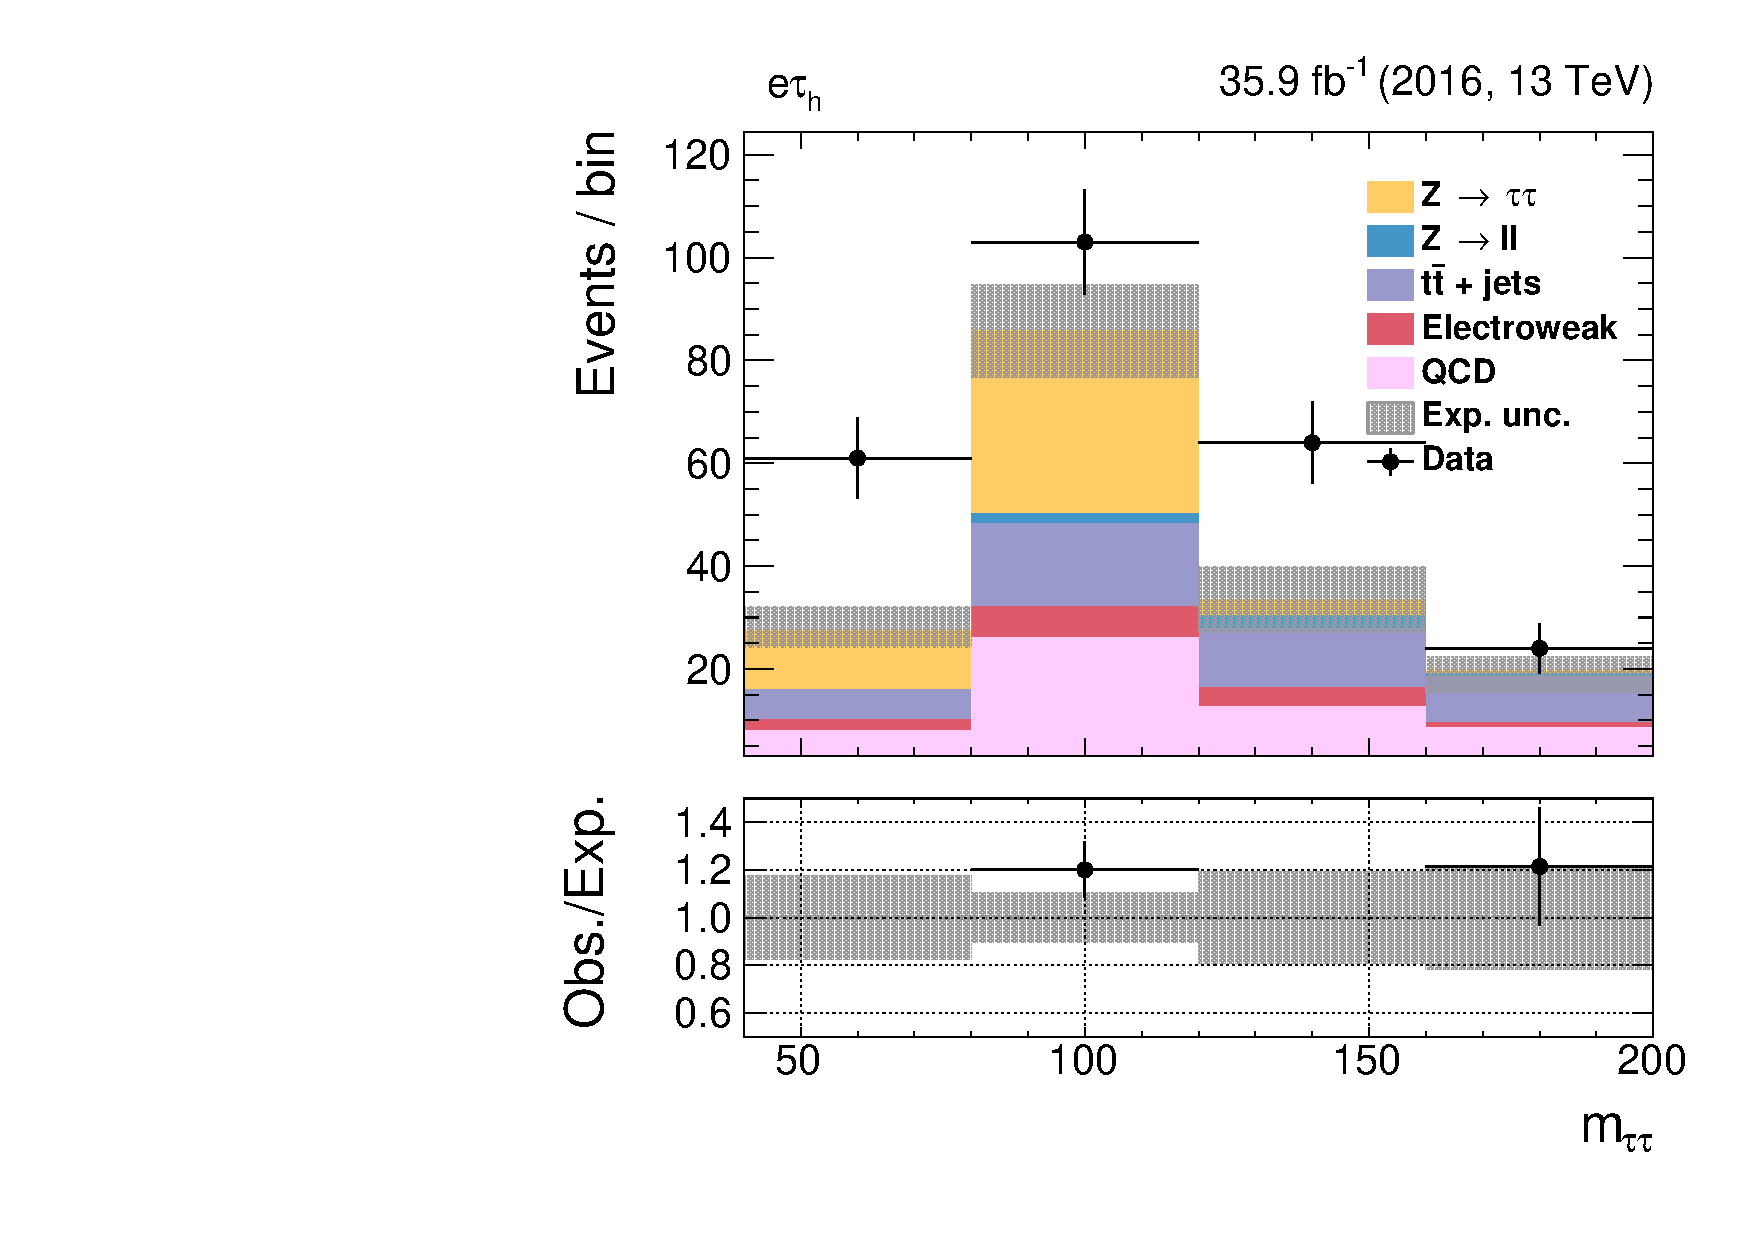
\includegraphics[width=0.47\textwidth]{Figures/background_estimation/RQCDOSSS/Postfit/et_dijet2D_antiiso_near/prefit_et_dijet2D_antiiso_near.pdf}}
  {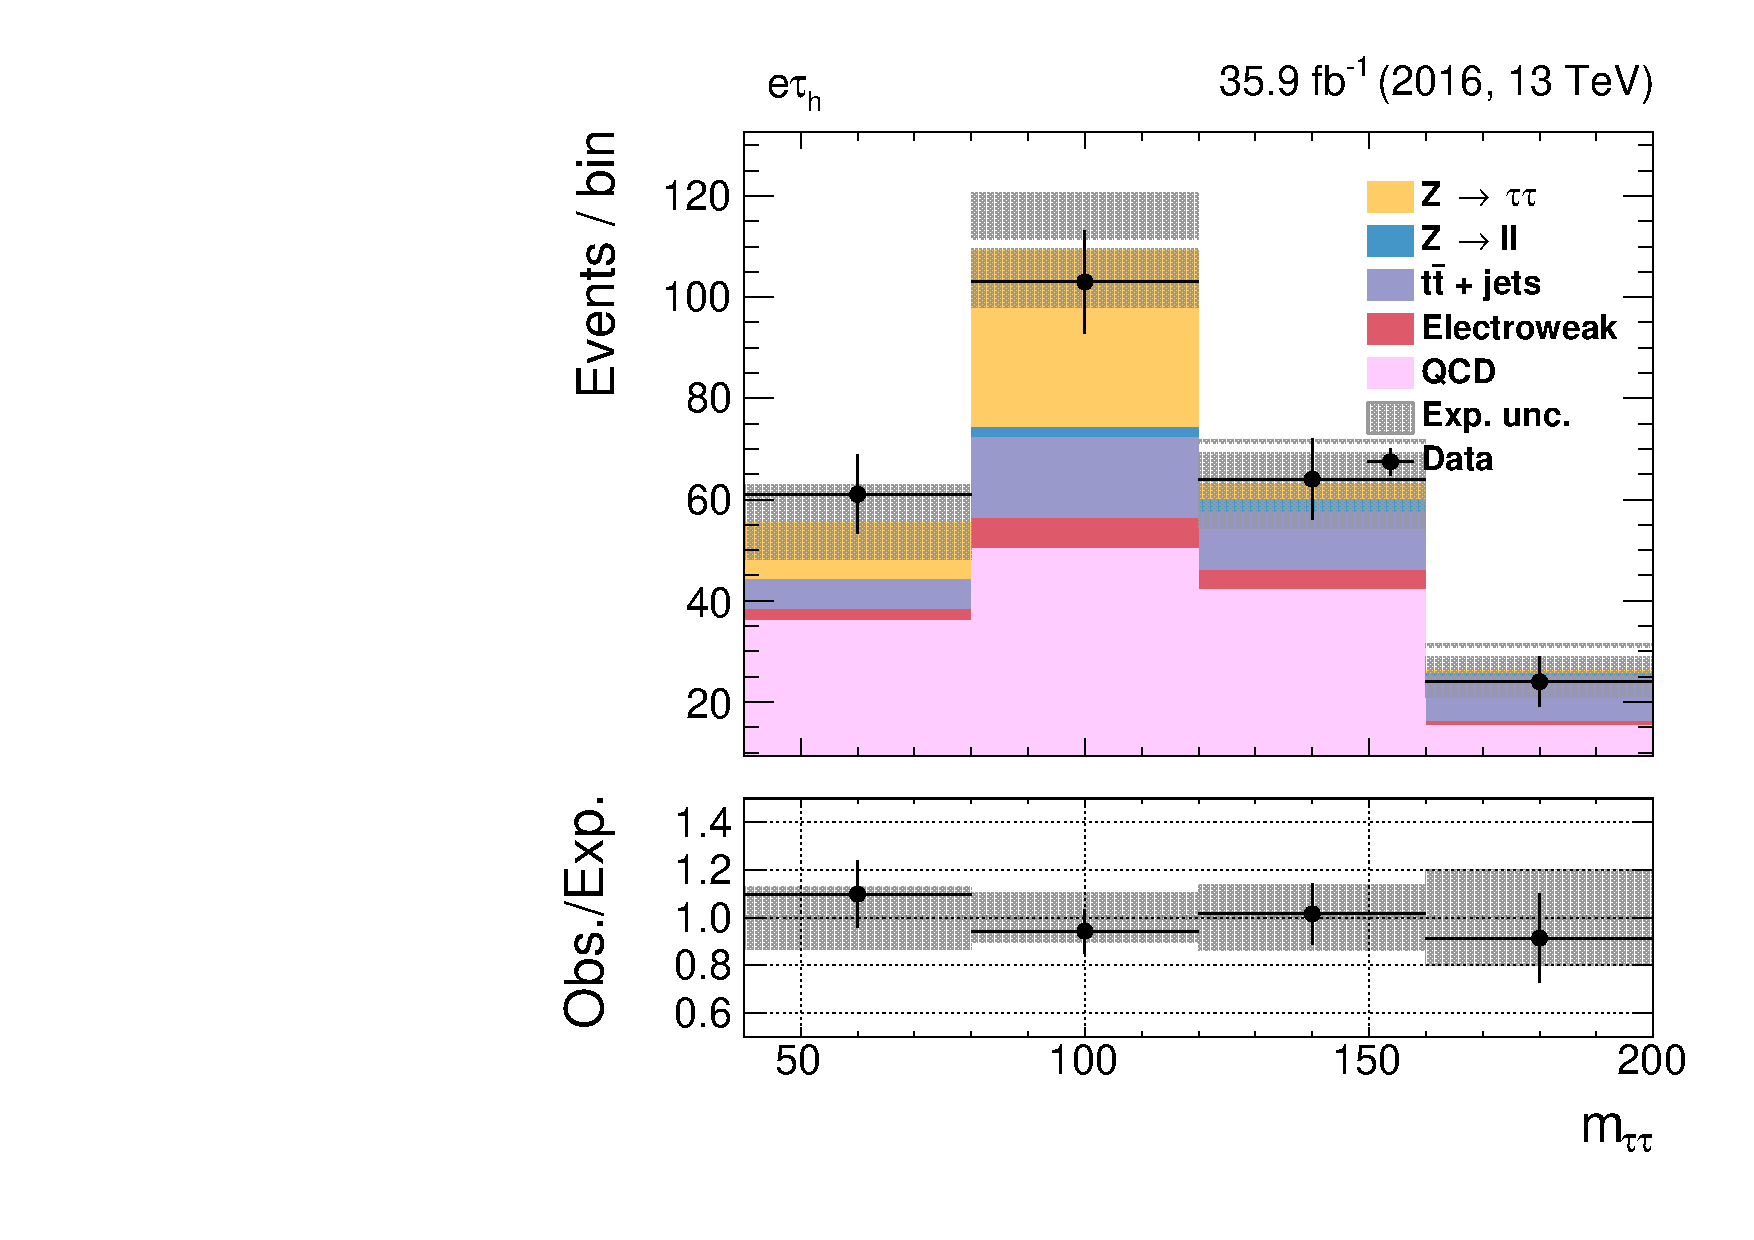
\includegraphics[width=0.47\textwidth]{Figures/background_estimation/RQCDOSSS/Postfit/et_dijet2D_antiiso_near/postfit_et_dijet2D_antiiso_near.pdf}}   
 \caption[Prefit and Postfit distributions in the $e\tau_\text{h}$ channel for the \textit{near} sideband.]{Prefit (left) and Postfit (right) distributions in the $e\tau_\text{h}$ channel for the \textit{near} sideband for the \textit{0-jet} (upper row), \textit{boosted} (middle row) and \textit{dijet} (bottom row) categories.
 During the fit, the QCD rate is pulled by the fit to find an optimal normalization of the background to describe data.}
 \label{fig:etmtqcd:et_prefitpostfit_near}
\end{figure}
\clearpage 
\begin{figure}[h!]
\centering
  {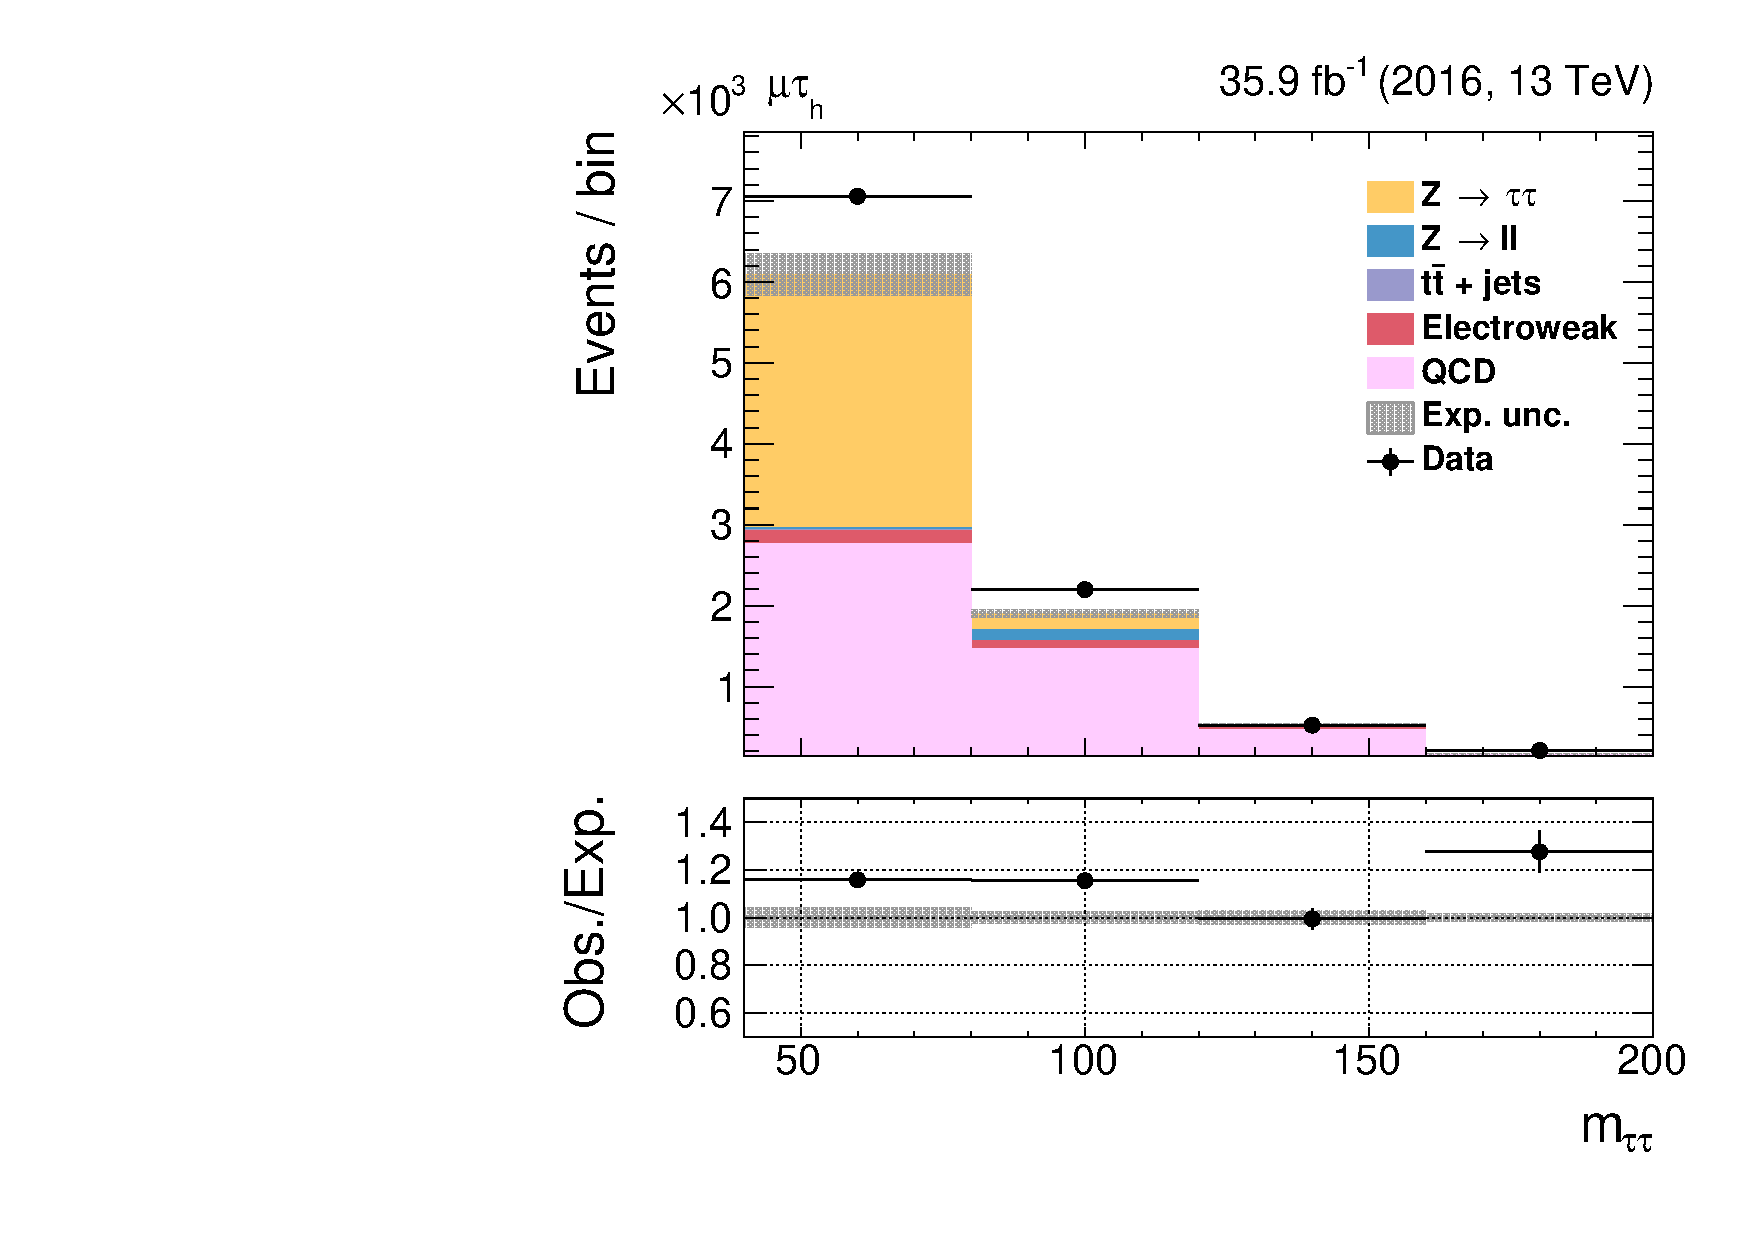
\includegraphics[width=0.47\textwidth]{Figures/background_estimation/RQCDOSSS/Postfit/mt_ZeroJet2D_antiiso_near/prefit_mt_ZeroJet2D_antiiso_near.pdf}}
  {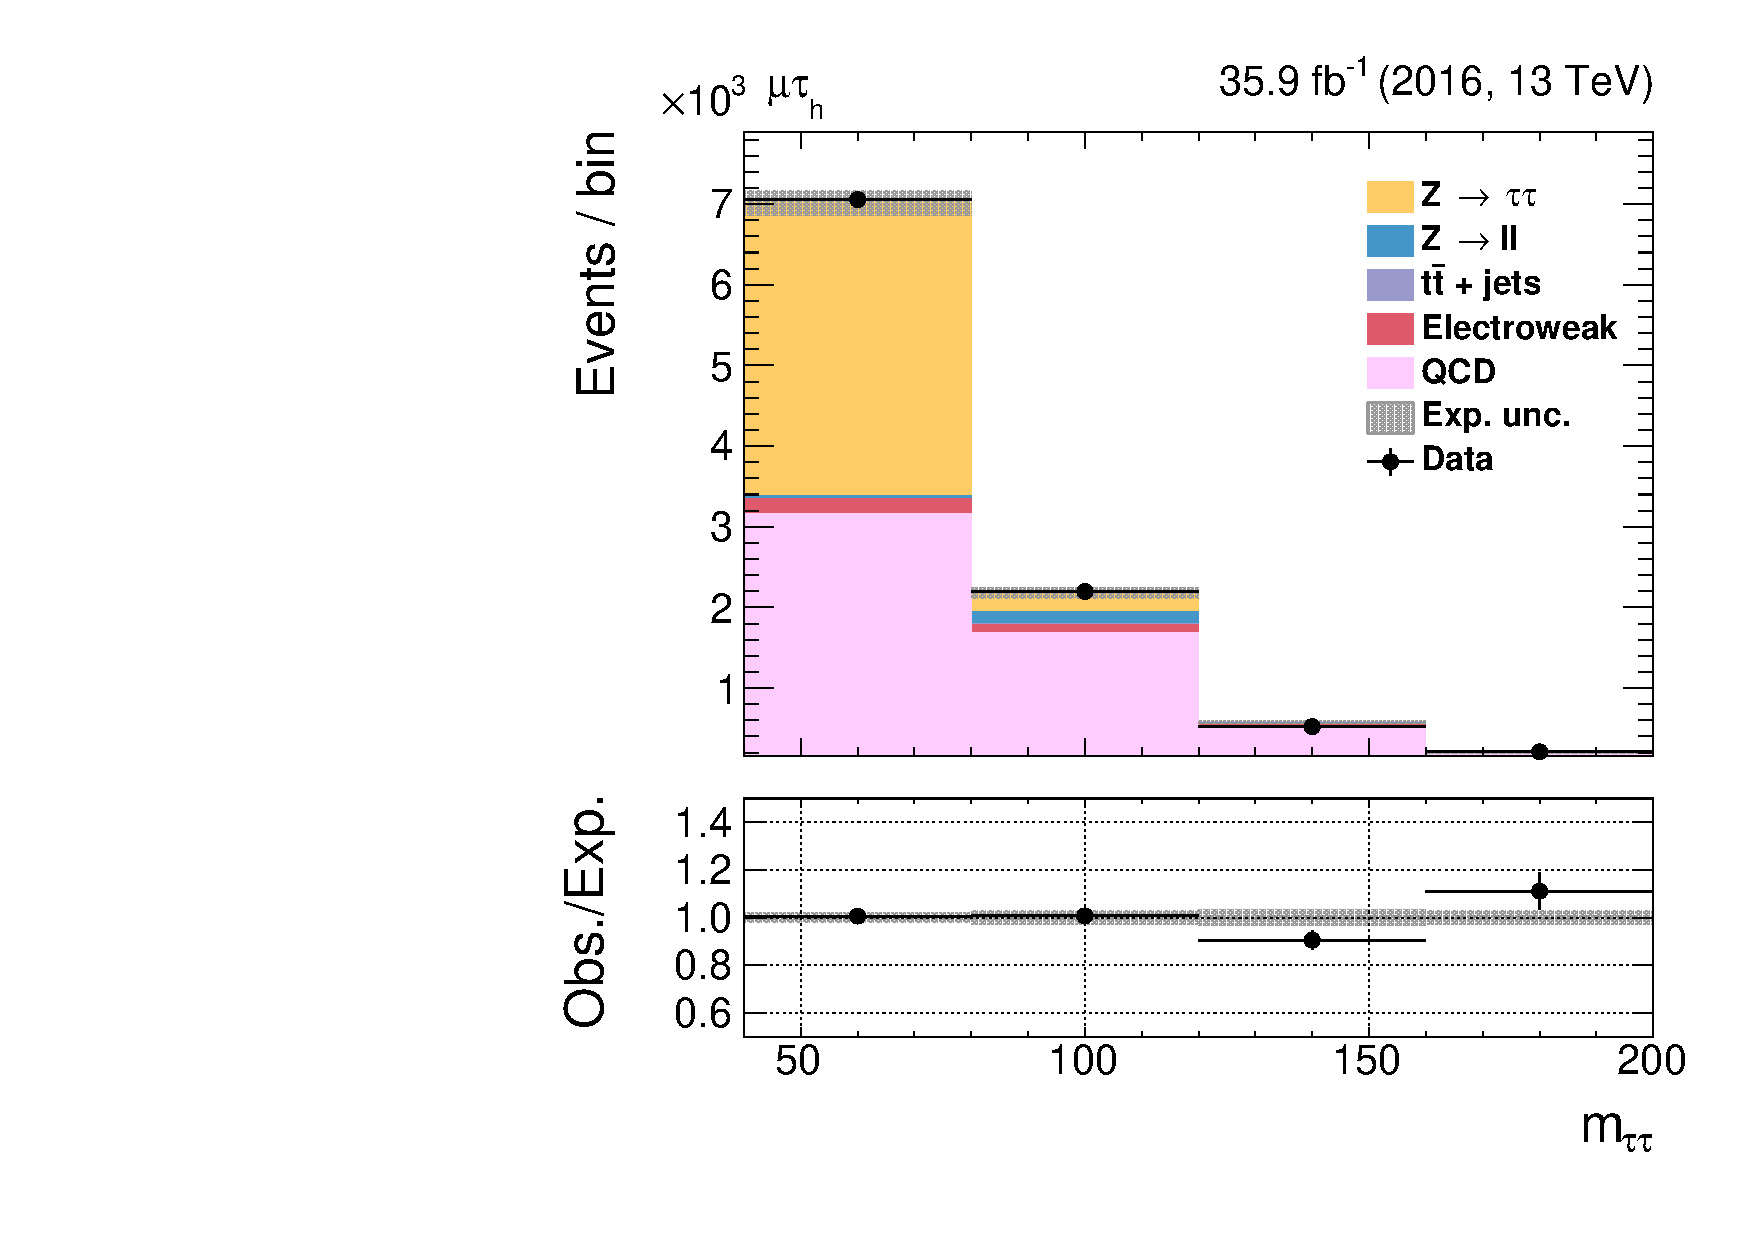
\includegraphics[width=0.47\textwidth]{Figures/background_estimation/RQCDOSSS/Postfit/mt_ZeroJet2D_antiiso_near/postfit_mt_ZeroJet2D_antiiso_near.pdf}} \\ 
  {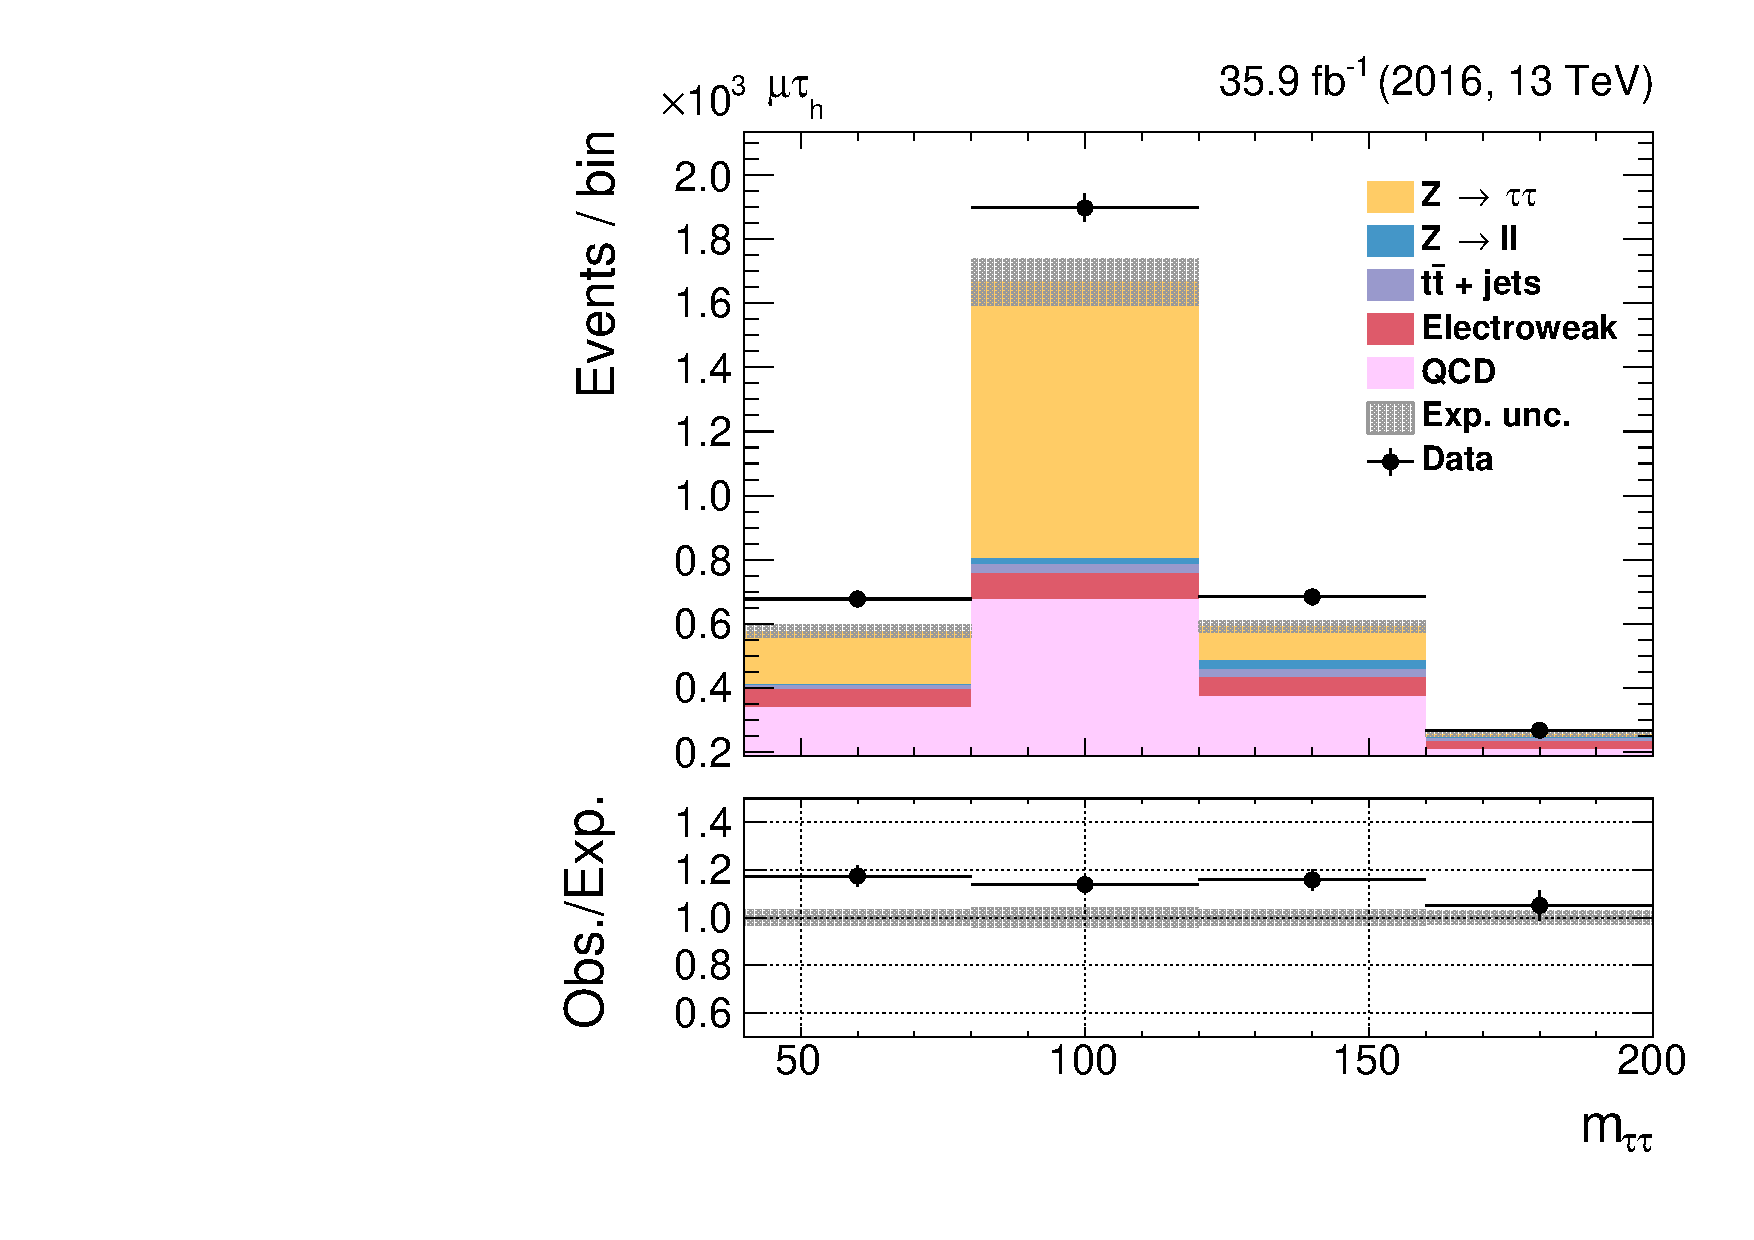
\includegraphics[width=0.47\textwidth]{Figures/background_estimation/RQCDOSSS/Postfit/mt_Boosted2D_antiiso_near/prefit_mt_Boosted2D_antiiso_near.pdf}}
  {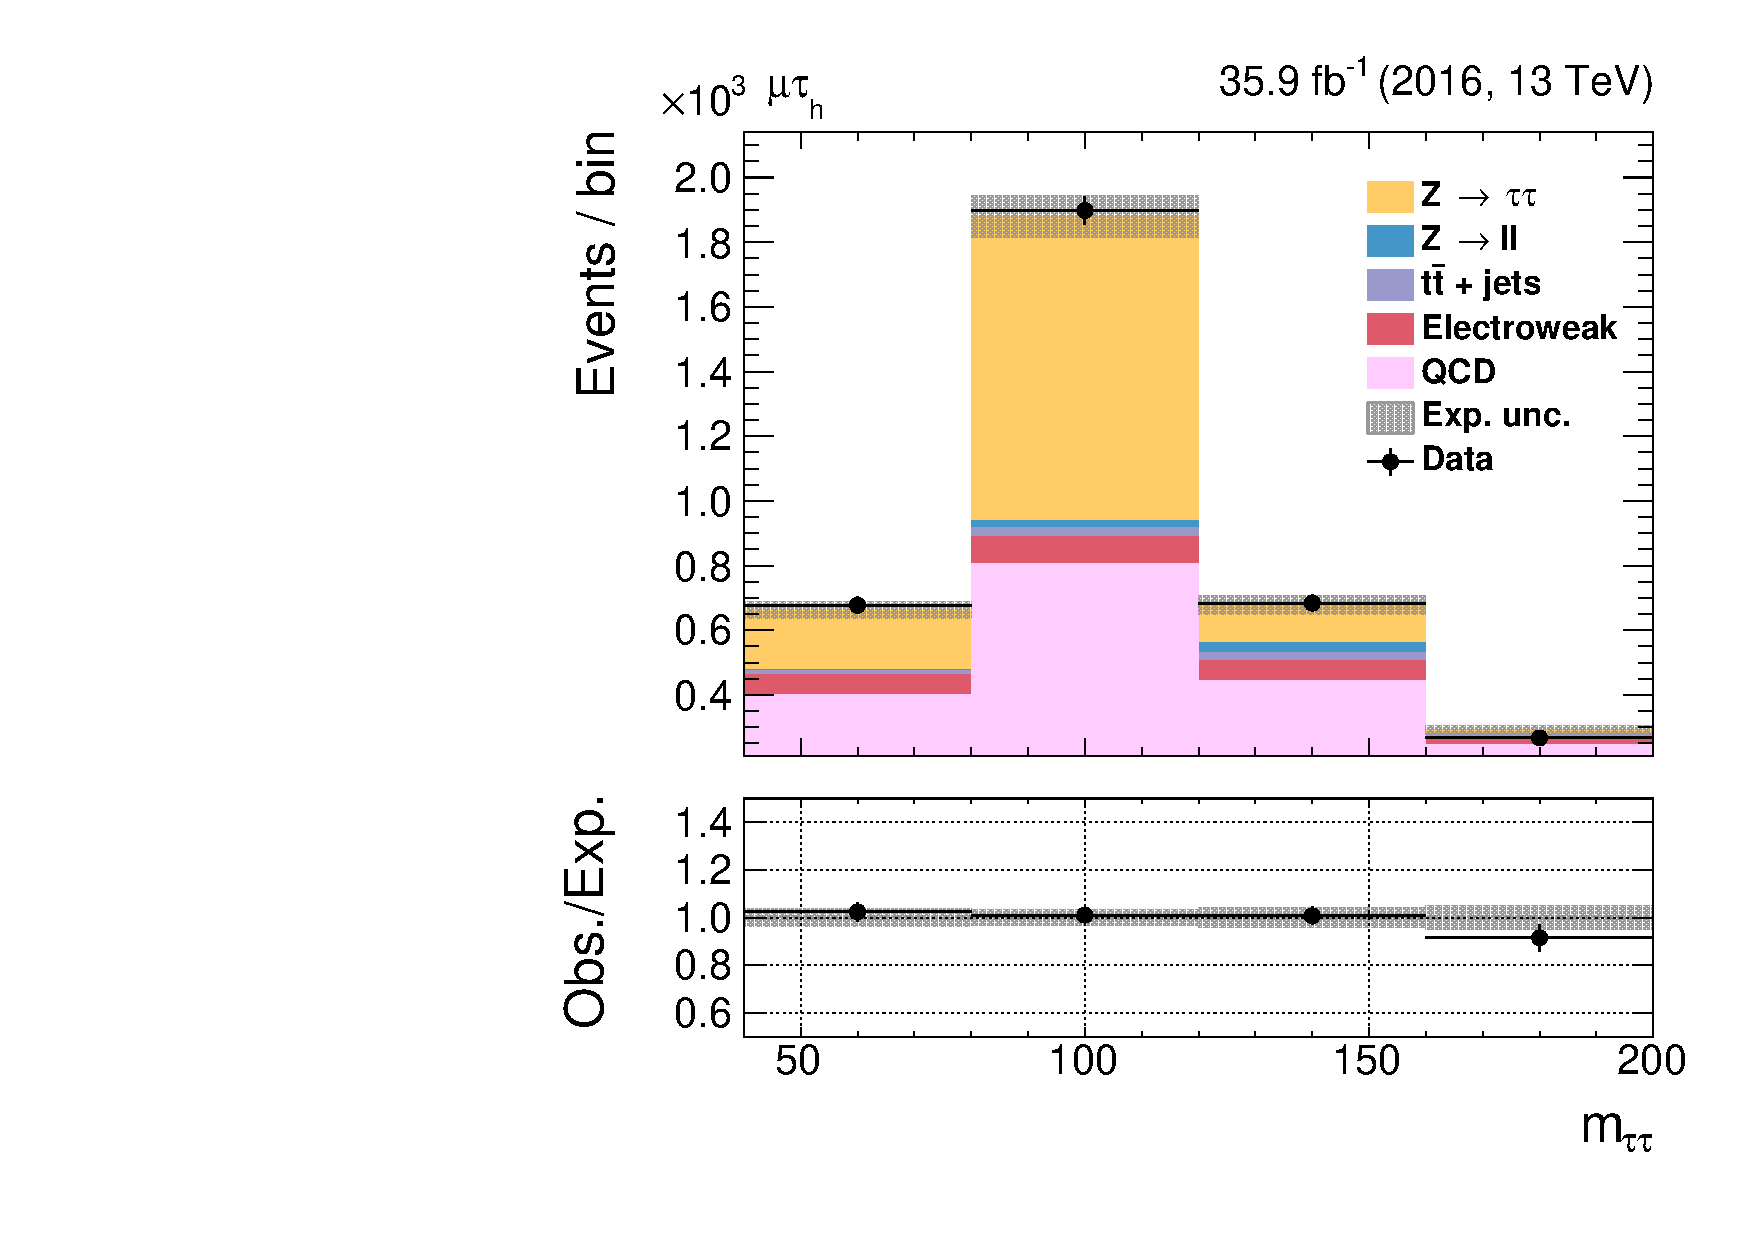
\includegraphics[width=0.47\textwidth]{Figures/background_estimation/RQCDOSSS/Postfit/mt_Boosted2D_antiiso_near/postfit_mt_Boosted2D_antiiso_near.pdf}} \\
  {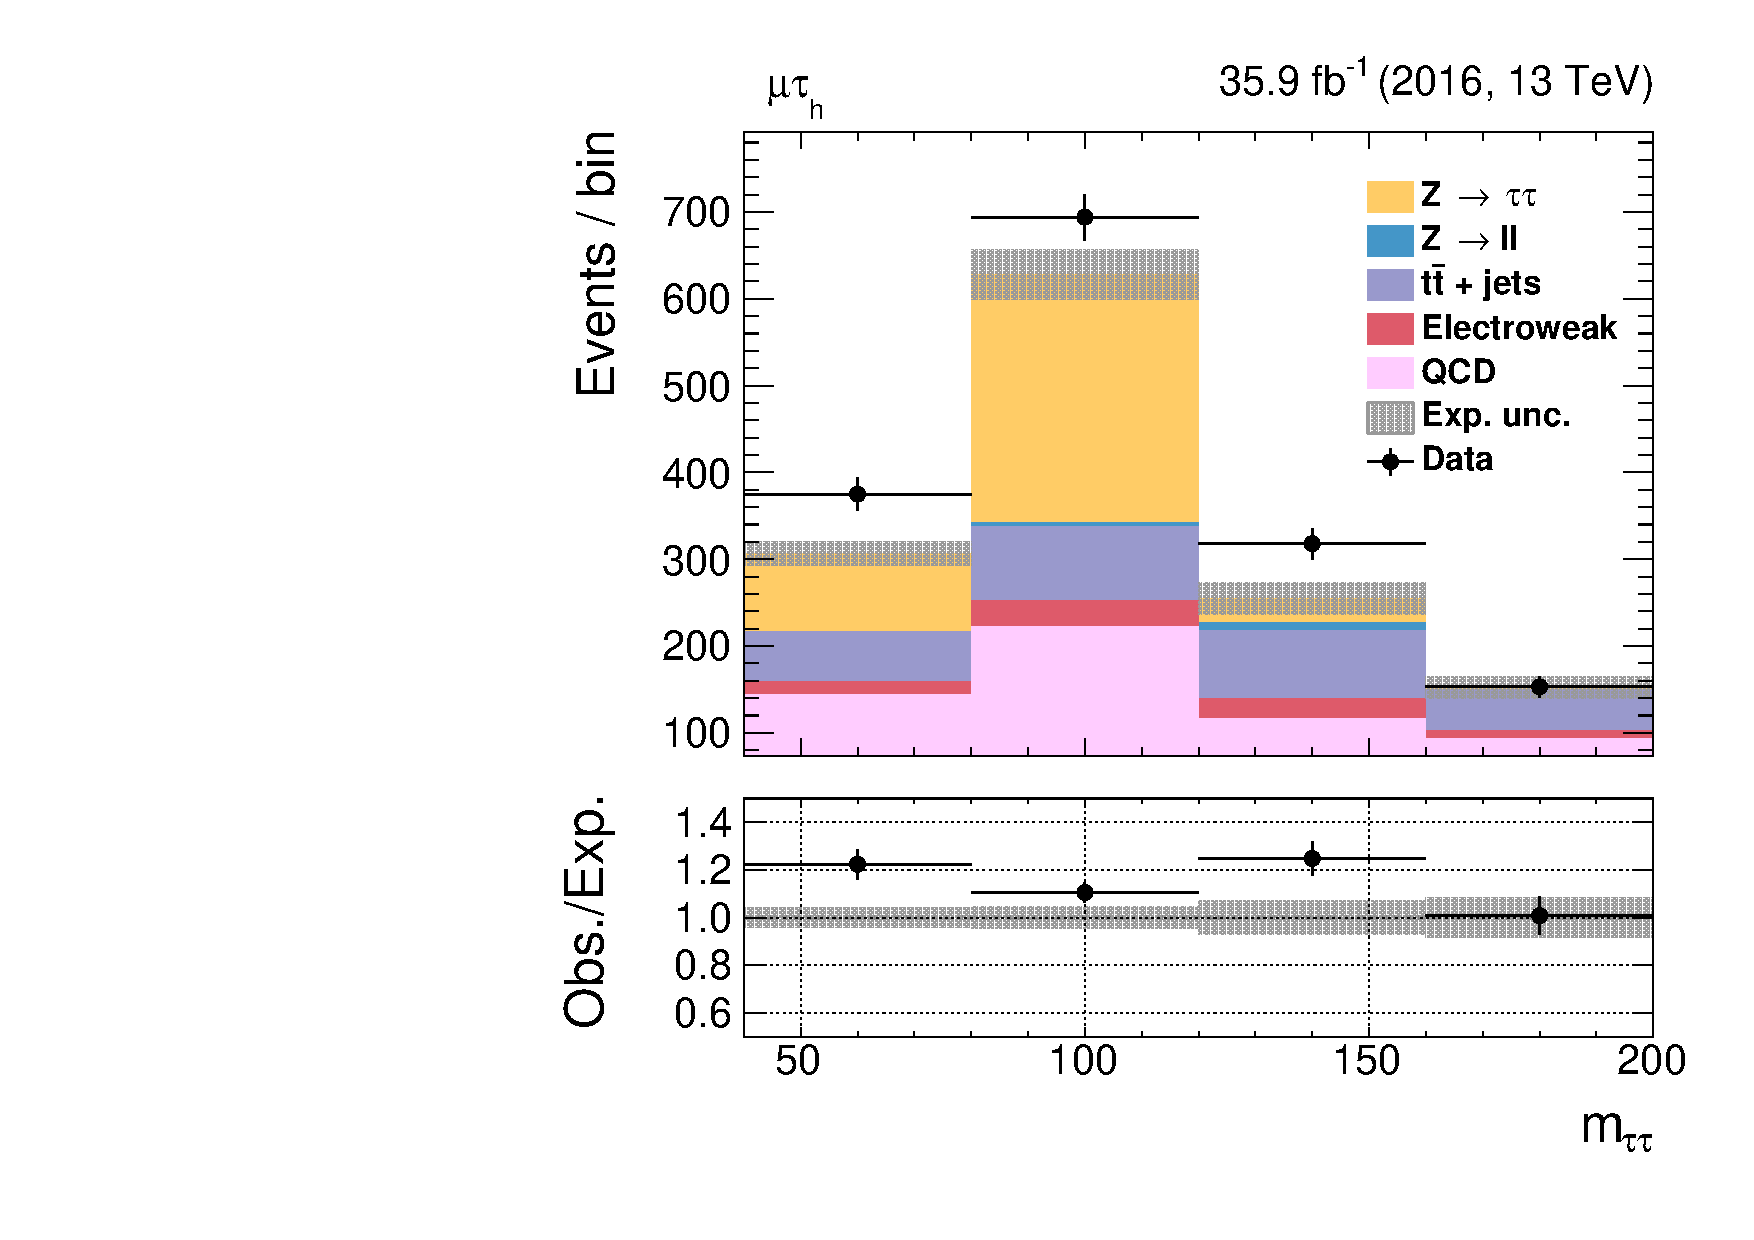
\includegraphics[width=0.47\textwidth]{Figures/background_estimation/RQCDOSSS/Postfit/mt_dijet2D_antiiso_near/prefit_mt_dijet2D_antiiso_near.pdf}}
  {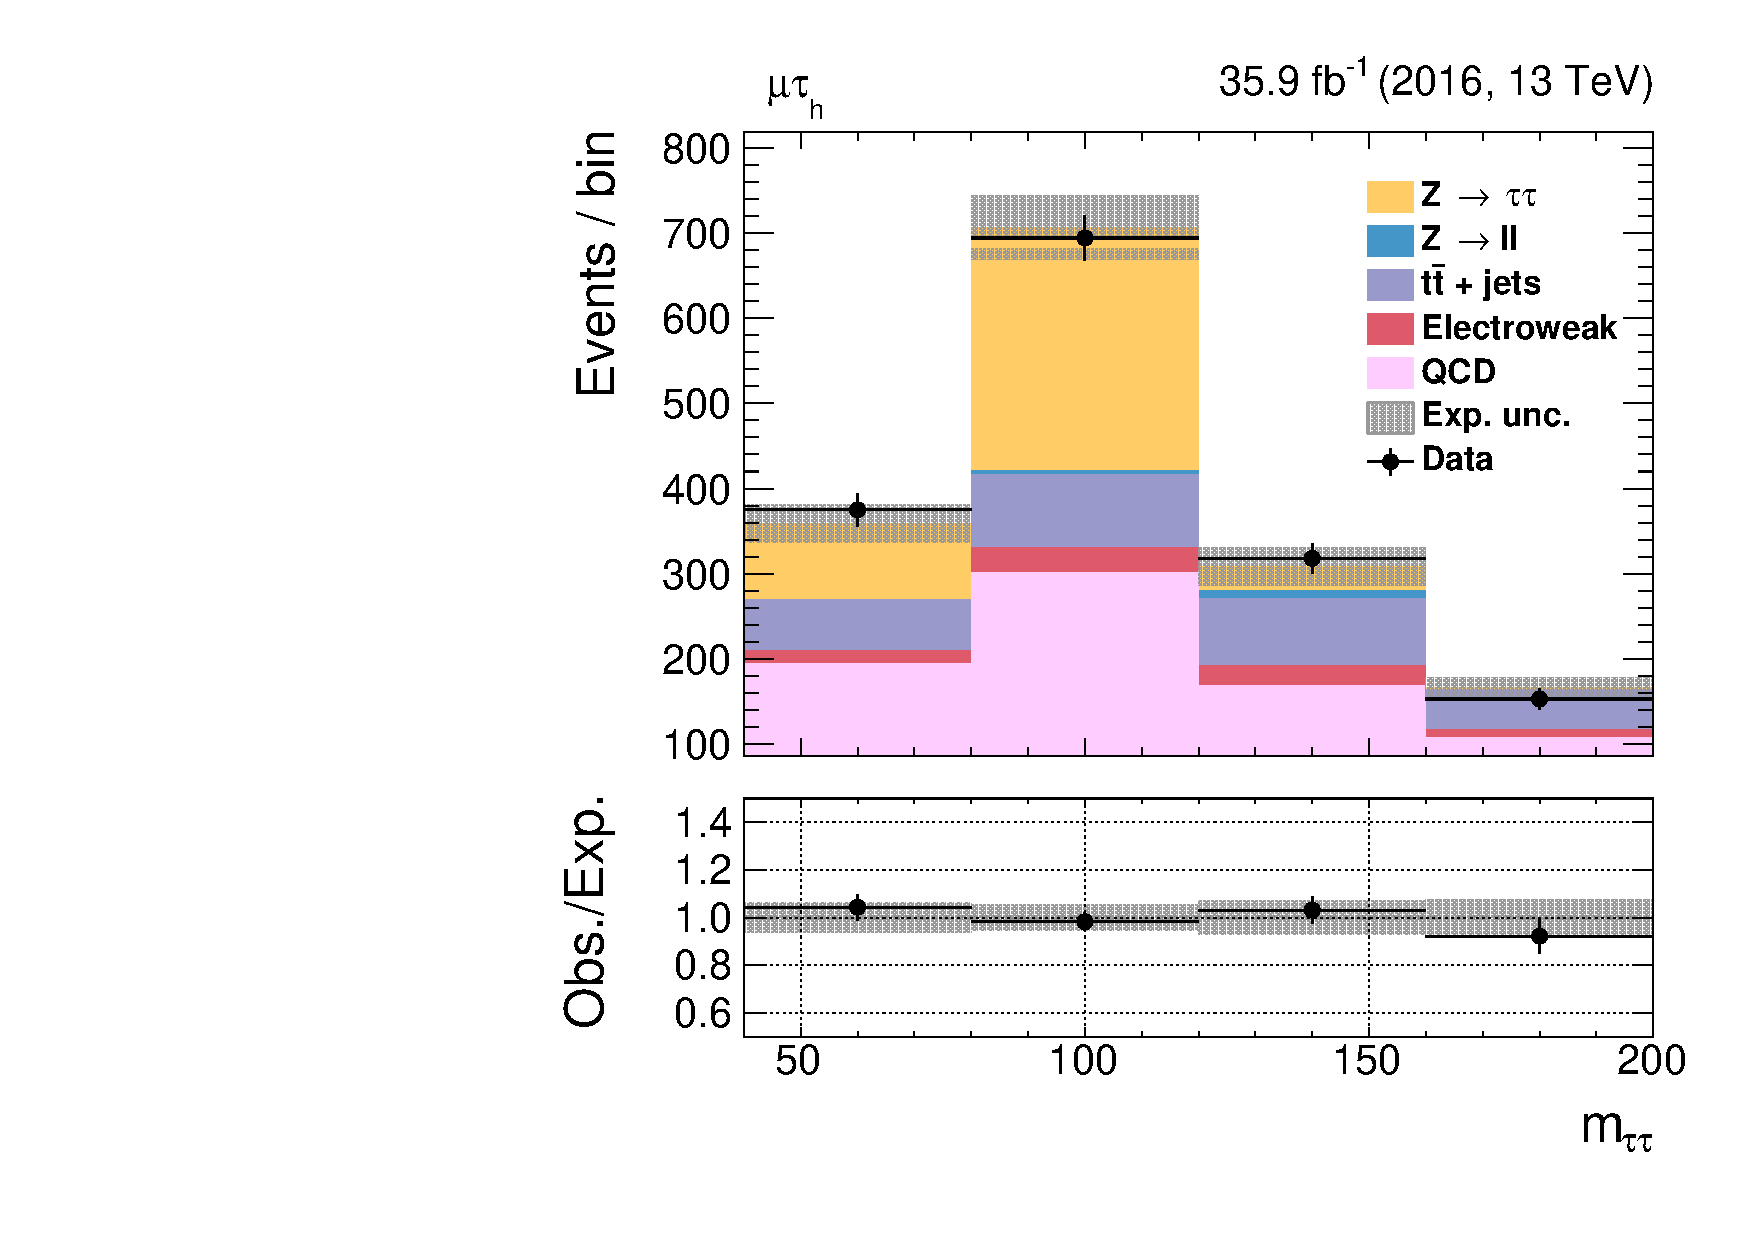
\includegraphics[width=0.47\textwidth]{Figures/background_estimation/RQCDOSSS/Postfit/mt_dijet2D_antiiso_near/postfit_mt_dijet2D_antiiso_near.pdf}}   
 \caption[Prefit and Postfit distributions in the $\mu\tau_\text{h}$ channel for the \textit{near} sideband.]{Prefit (left) and postfit (right) distributions in the $\mu\tau_\text{h}$ channel for the \textit{near} sideband for the \textit{0-jet} (upper row), \textit{boosted} (middle row) and \textit{dijet} (bottom row) categories.
 During the fit, the QCD rate is pulled by the fit to find an optimal normalization of the background to describe data.}\label{fig:etmtqcd:mt_prefitpostfit_near}
\end{figure}

\clearpage

 \paragraph{QCD control regions}\mbox{}\\
 For all signal categories one QCD control region is included to the final fit to constrain the QCD yield in the $e\tau_\text{h}$ and $\mu\tau_\text{h}$ channels.
 These control regions require the charges of the tau-plus-lepton pair to have the same sign. All other cuts defining the selection in the signal region are kept fixed. 
 Examples of these control regions are shown in figure \ref{fig:etmtqcd:0jet_qcd_control}. More plots can be found in the appendix in \figreft{supp_fig:etmtqcd:1jet_qcd_control}.

\begin{figure}[h!]
     \centering
     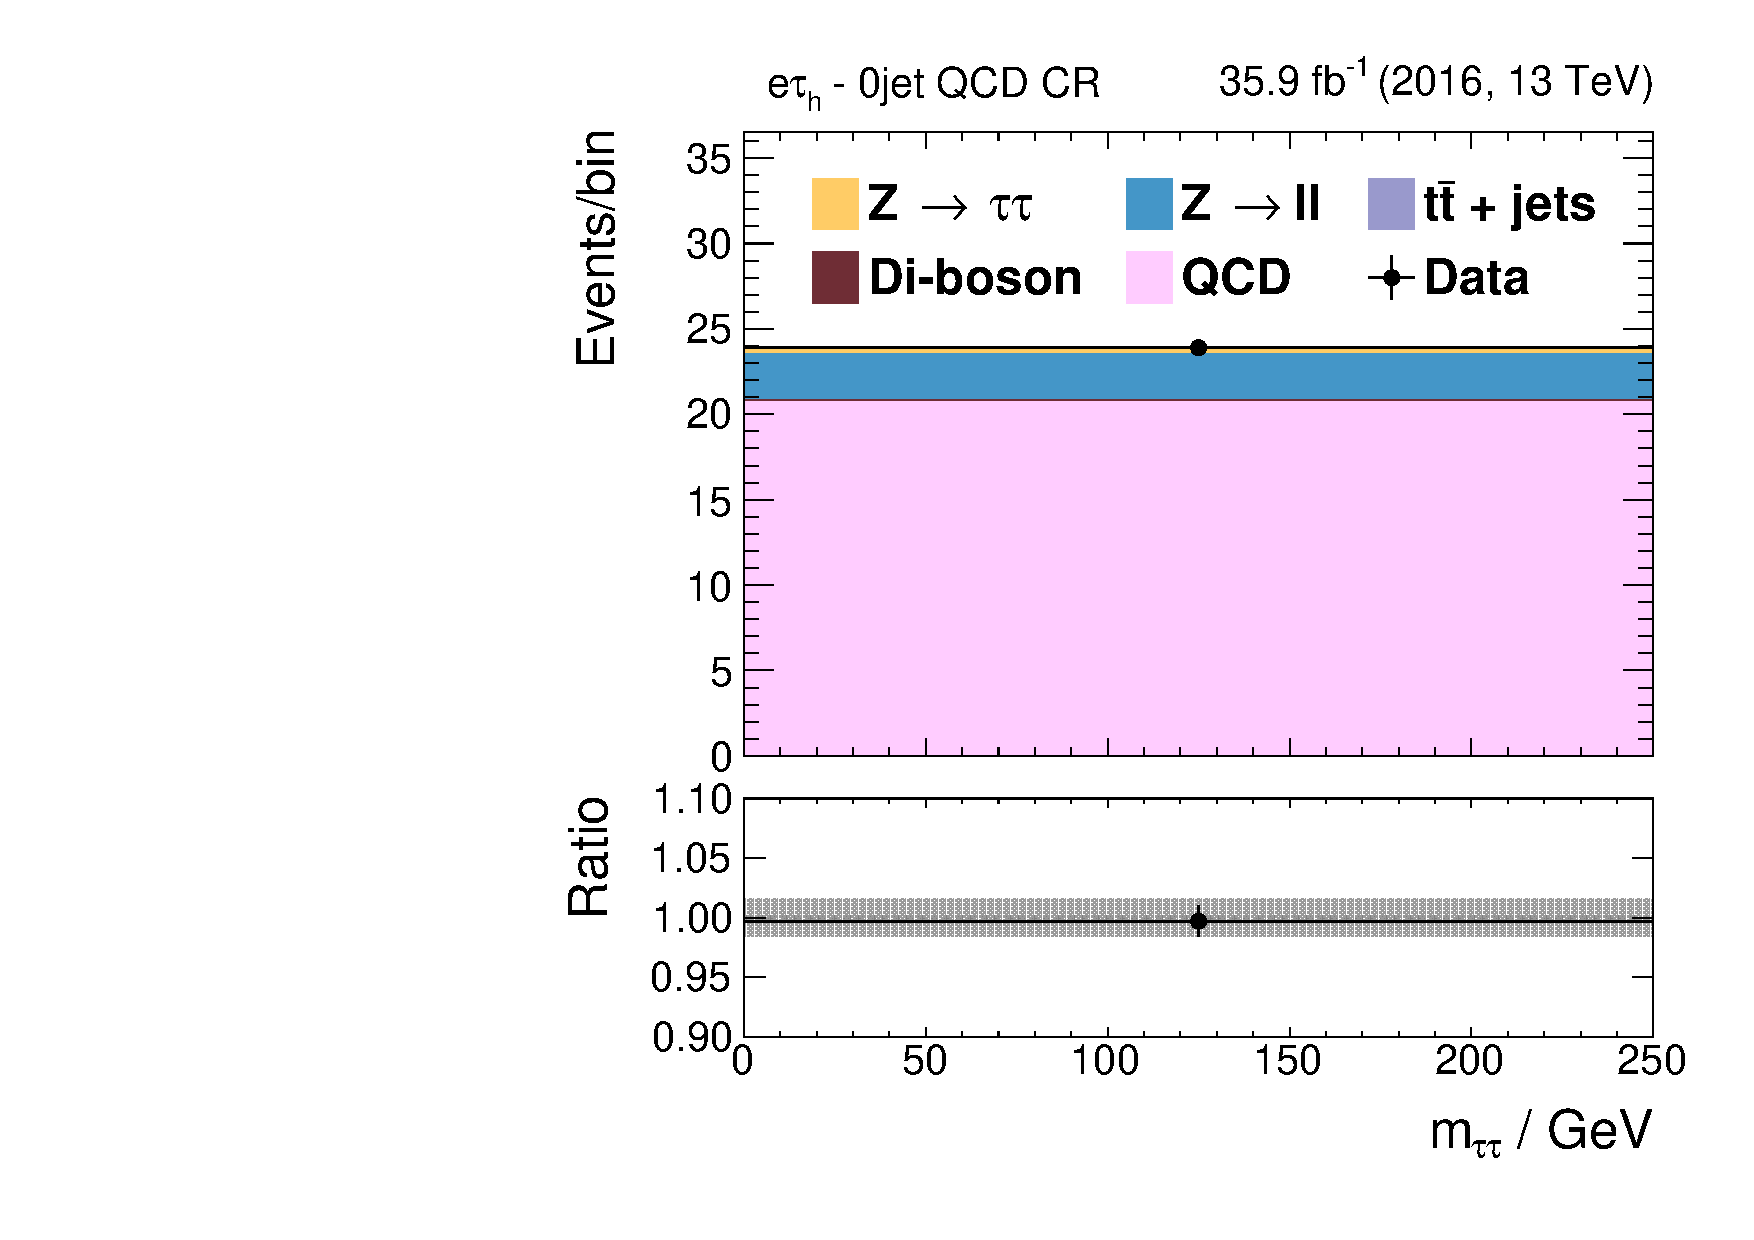
\includegraphics[width=0.47\textwidth]{Figures/background_estimation/qcd_et_control-regions/htt_inputet11__htt_et_11_13TeV.pdf}
     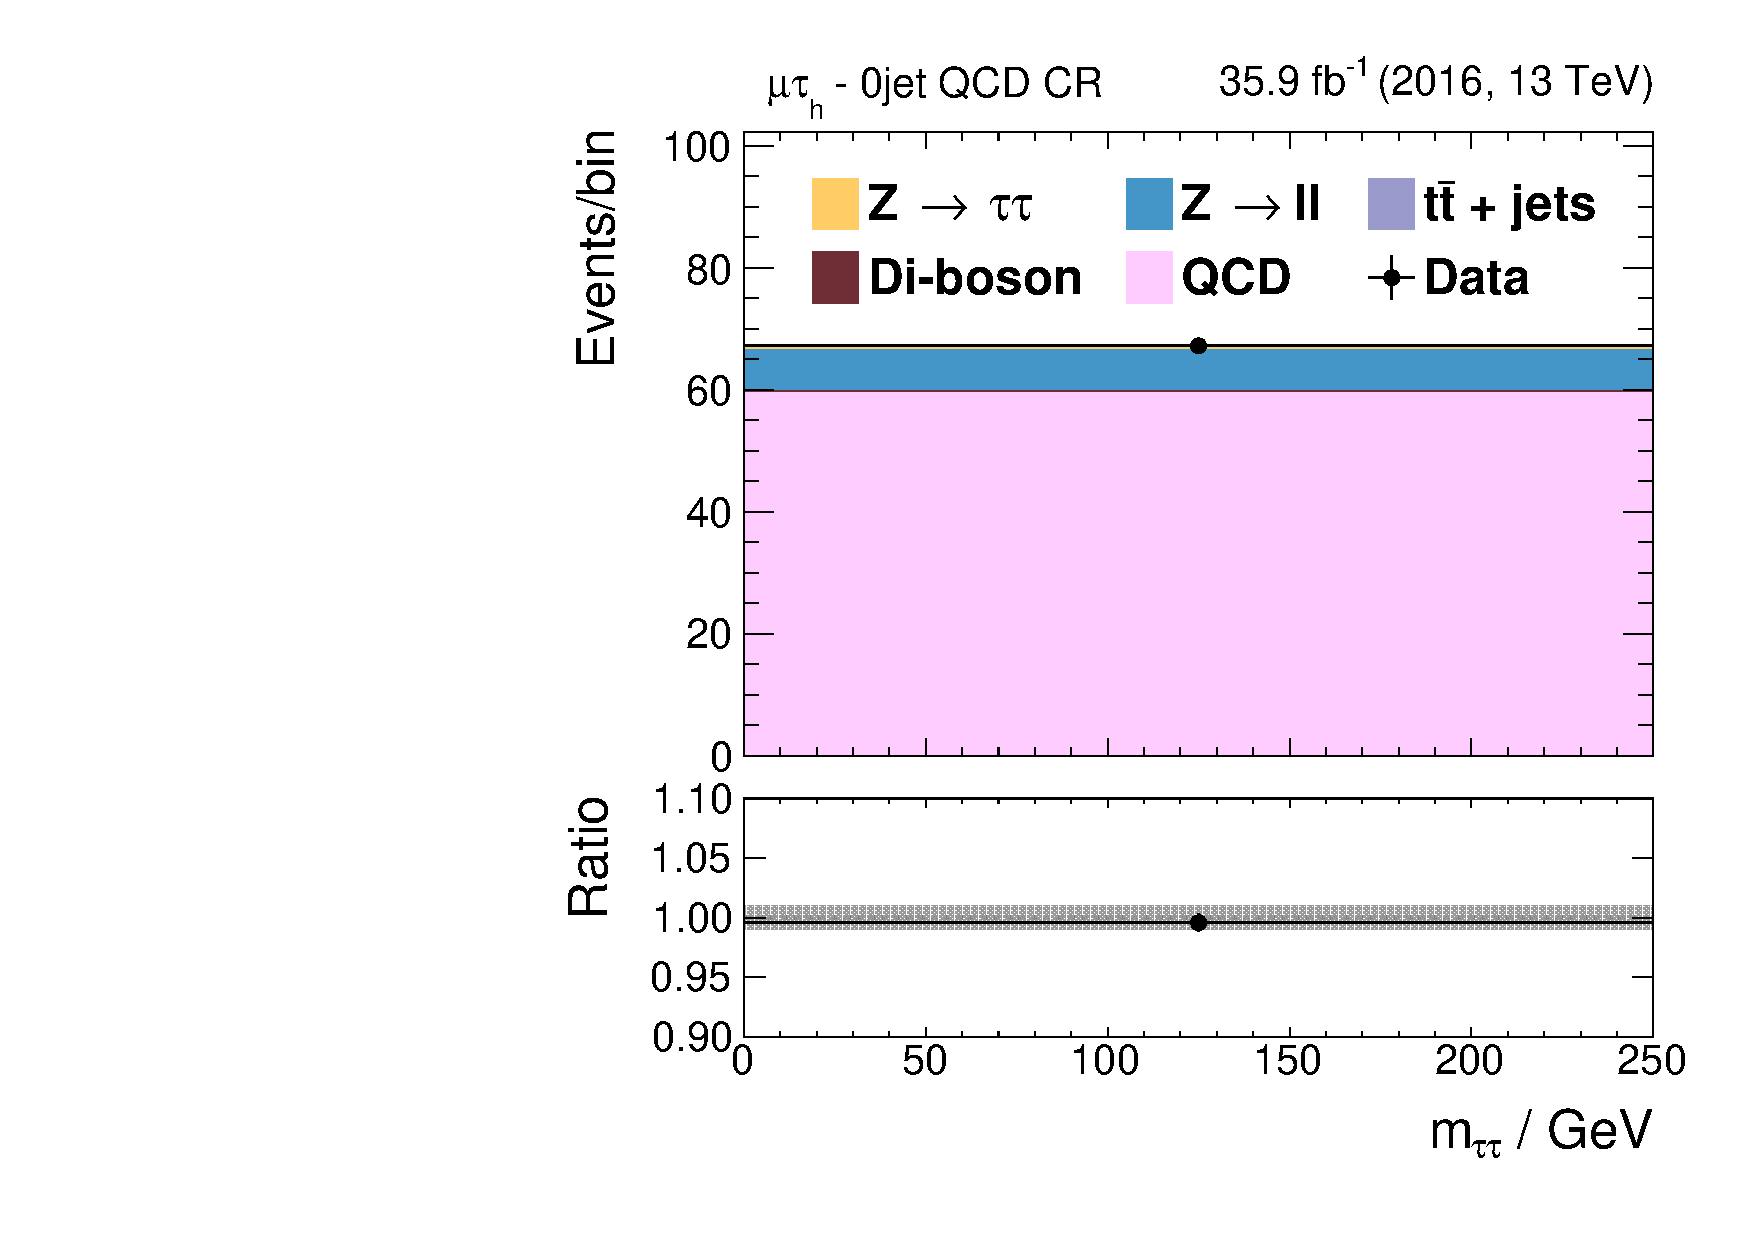
\includegraphics[width=0.47\textwidth]{Figures/background_estimation/qcd_mt_control-regions/htt_inputmt11__htt_mt_11_13TeV.pdf} \\
     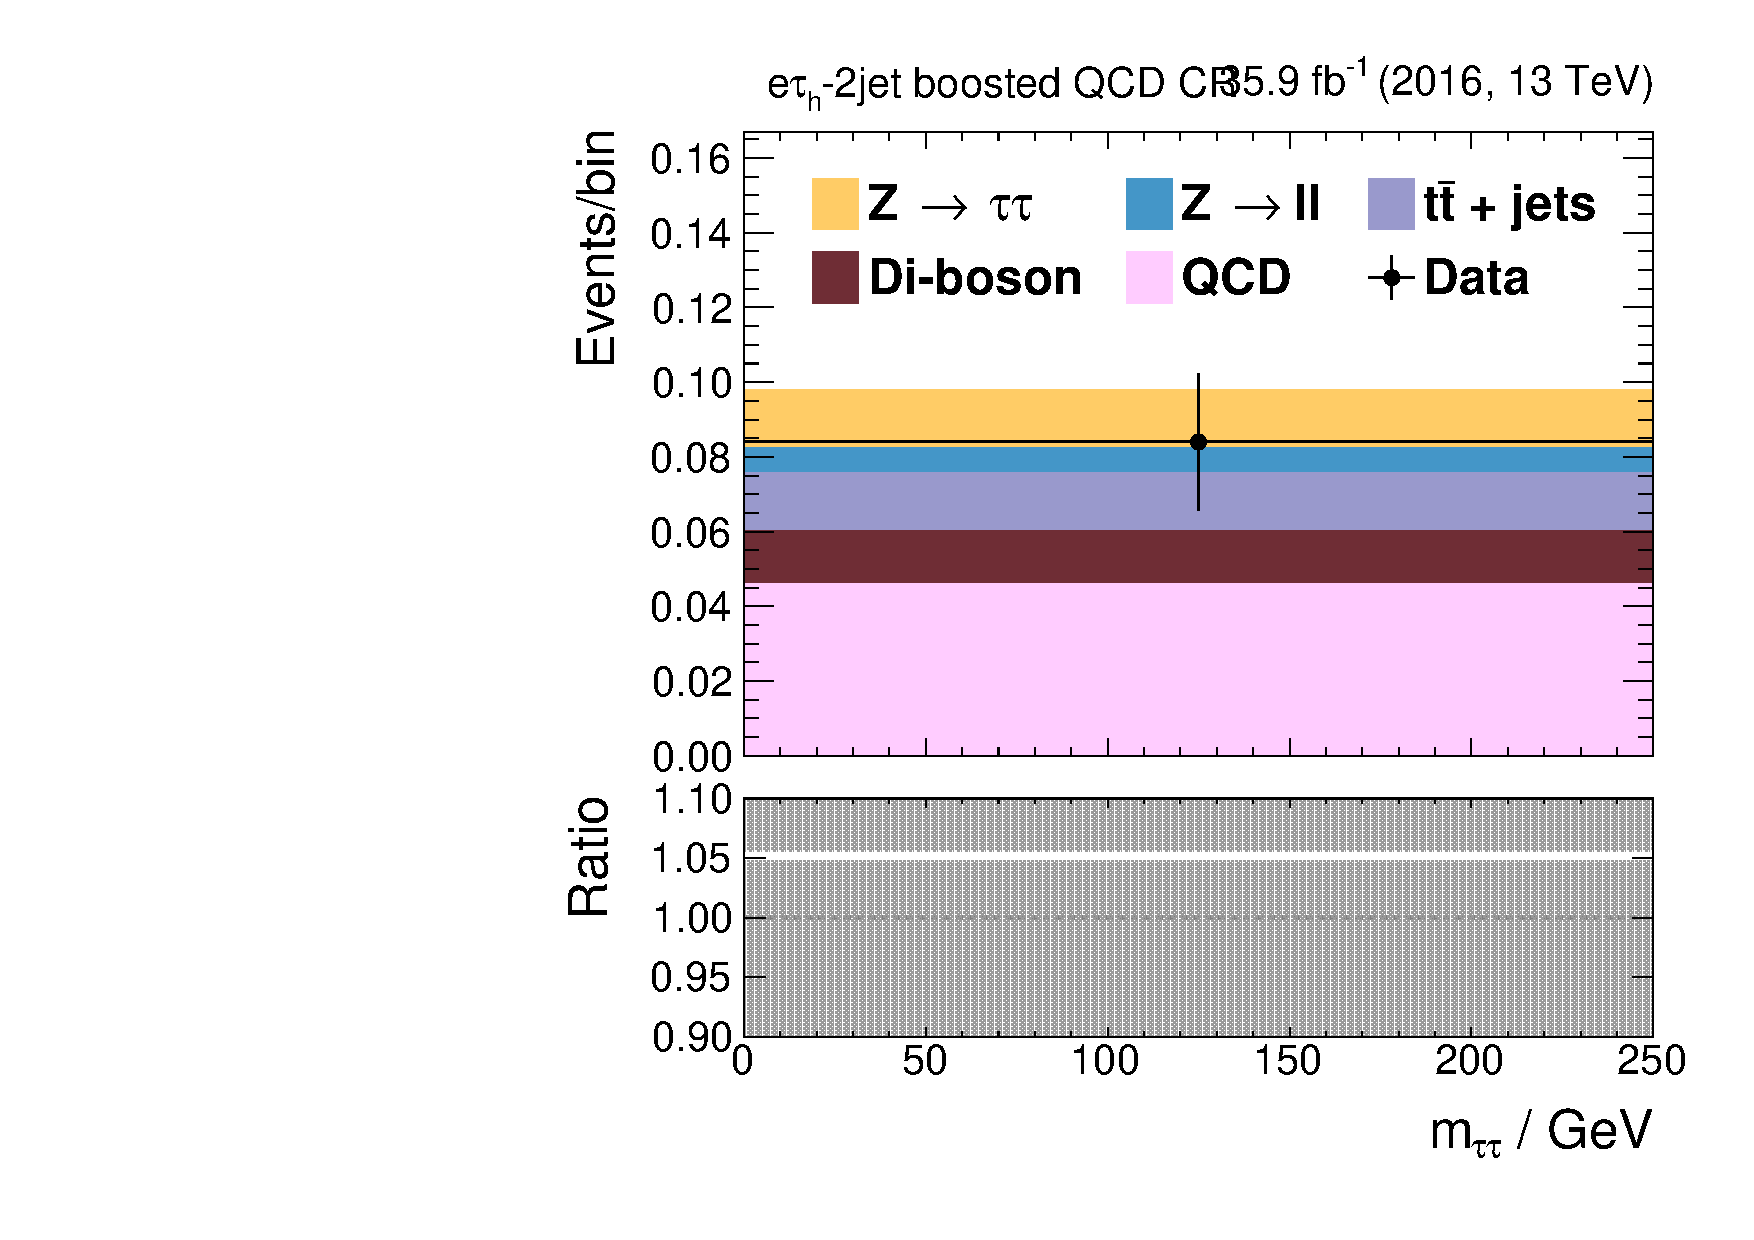
\includegraphics[width=0.47\textwidth]{Figures/background_estimation/qcd_et_control-regions/htt_inputet20__htt_et_20_13TeV.pdf}
     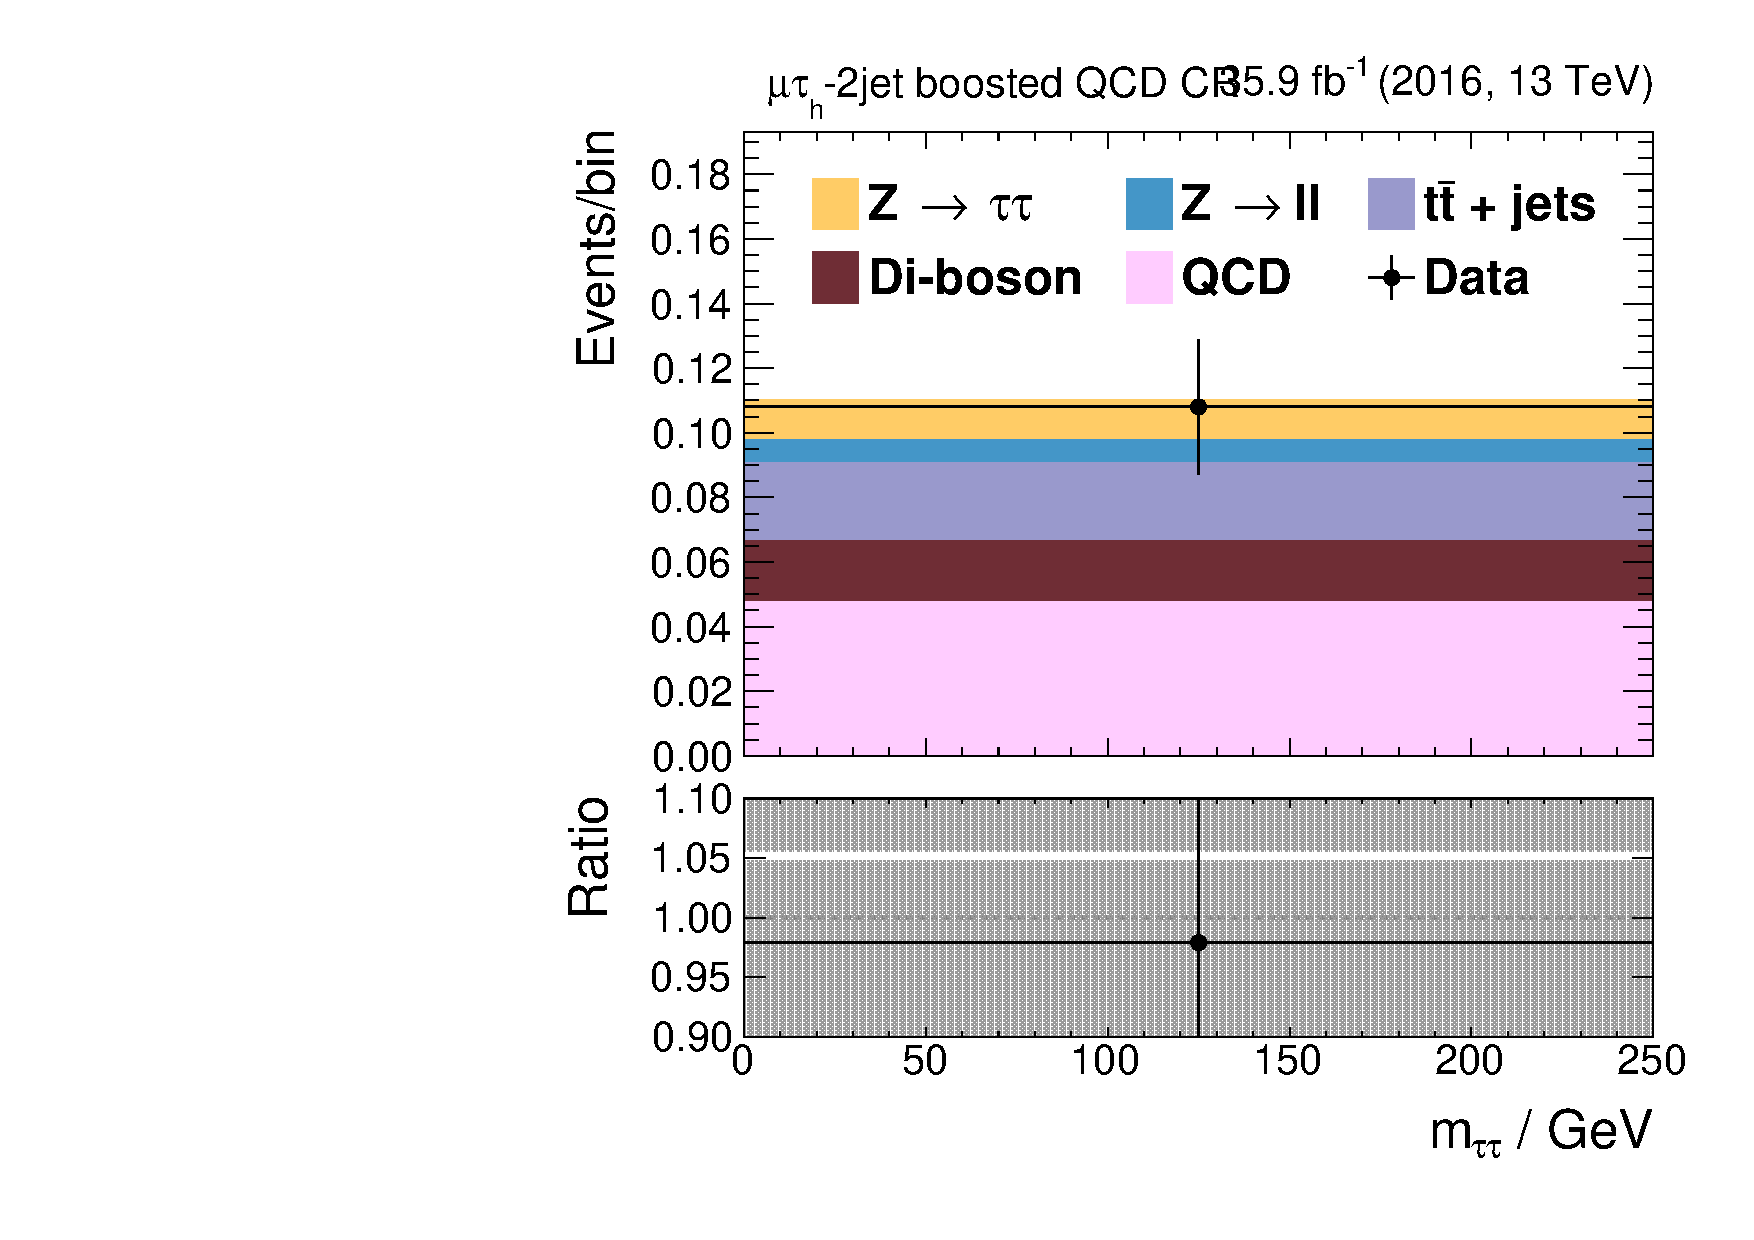
\includegraphics[width=0.47\textwidth]{Figures/background_estimation/qcd_mt_control-regions/htt_inputmt20__htt_mt_20_13TeV.pdf} 
  \caption[QCD control region in the \textit{0-jet} and \textit{dijet boosted} category.]{Background modeling and data in the QCD control region in the \textit{0-jet} category (upper row) and the \textit{dijet boosted} category (bottom row) for the $e\tau_\text{h}$ (left) and $\mu\tau_\text{h}$ (right) channel.}\label{fig:etmtqcd:0jet_qcd_control}
 \end{figure}%
 
\clearpage 

\subsubsection{$\tau_\text{h}\tau_\text{h}$ channel}
In the $\tau_\text{h}\tau_\text{h}$ channel QCD becomes a dominant background because quark or gluon jets are likely to be misidentified as hadronically decaying tau leptons.
\begin{figure}[h!]
    \centering
    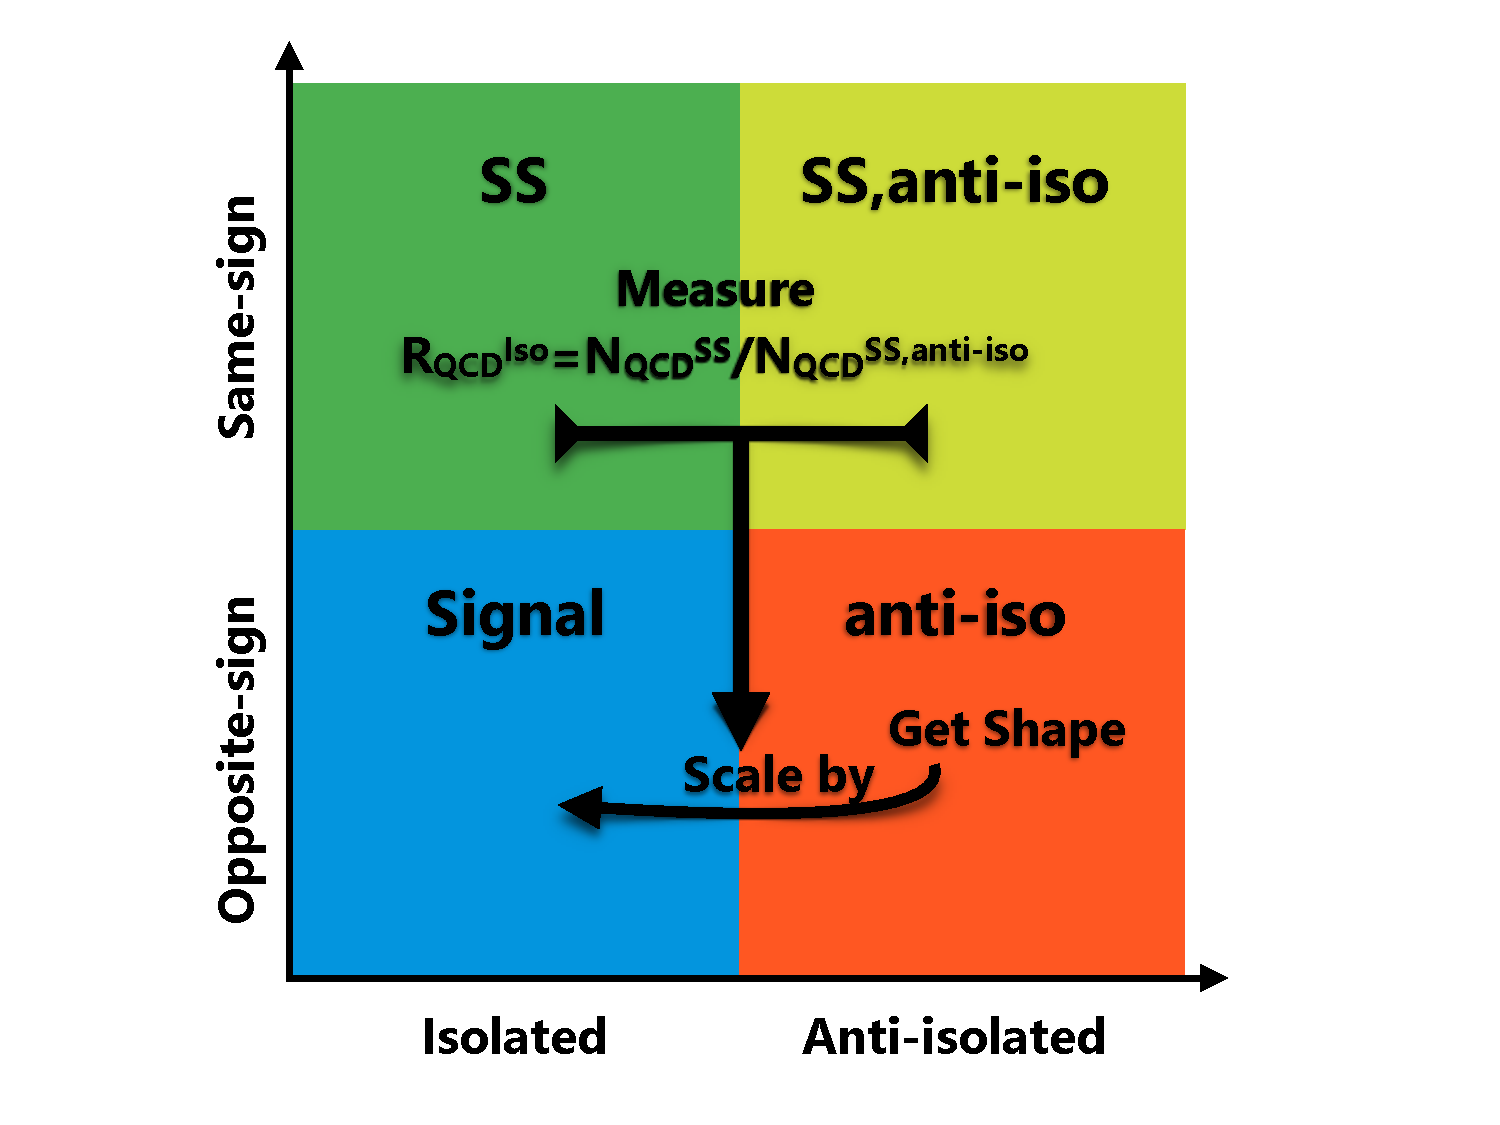
\includegraphics[width=.5\textwidth]{Figures/background_estimation/QCD_tt/ABCD_tauhadtauhad.pdf}
    \caption{Estimation procedure of the QCD background in the $\tau_\text{h}\tau_\text{h}$ channel. The control region in anti-isolated events is used to extract the shape of QCD from data. 
    The anti-isolated to isolated extrapolation factor $R_\text{QCD}^\text{iso}$ is measured in same-sign events. The factor scales the yield of the anti-isolated QCD estimate to the signal region giving the final estimate.}\label{BE:QCD:abcd_tauhadtauhad}
\end{figure} 
 
The multijet background in this channel is estimated from data in an anti-isolated control region as proposed in \cite{Sirunyan:2017khh}. 
For this, the working point (WP) of the isolation for one of the two hadronically decaying tau leptons is relaxed to pass the \textit{medium} WP of the MVA-based tau ID, which describes the tau lepton candidate isolation,
while simultaneously the isolation of the other $\tau_\text{h}$ is inverted, meaning that only tau leptons that do not pass the \textit{tight} WP are selected. In any case, the loose working point must be passed by both tau leptons.
The condition for the control region is 
\begin{align}
    I_{\tau_\text{h},1} != \text{tight WP} \tab \& \tab  I_{\tau_\text{h},1} &= \text{loose WP}  \tab \& \tab  I_{\tau_\text{h},2} = \text{medium WP} \tab \text{or} \\
    I_{\tau_\text{h},2} != \text{tight WP} \tab \& \tab  I_{\tau_\text{h},2} &= \text{loose WP}  \tab \& \tab  I_{\tau_\text{h},1} = \text{medium WP}.
\end{align}
By inverting the tight WP of one of the $\tau_\text{h}$'s it is ensured that no overlap exists with tau leptons that enter the signal regions. The relaxation of the other \tauh{} leads more events in the sideband regions, giving statistically more robust results.
Furthermore, another sideband is constructed by inverting the requirement that the two tau leptons must have oppositely signed electric charges (see \figreft{BE:QCD:abcd_tauhadtauhad}).
Backgrounds taken from simulation are subtracted from data in both isolated and anti-isolated sideband regions to obtain the number of multijet events.
This SS sideband is used to calculate the ratio of isolated to anti-isolated multijet events
\begin{equation}\label{BE:QCD:tt:eq}
    R_\text{QCD}^\text{iso} = \frac{N_\text{QCD}^\text{SS}}{N_\text{QCD}^\text{SS,anti-iso}} = \frac{N_\text{data}^\text{SS} - \sum_i N_{\text{bkg},i}^\text{SS}}{N_\text{data}^\text{SS,anti-iso} \sum_i N_{\text{bkg},i}^\text{SS,anti-iso}},
\end{equation} 
yielding the scale factors in \tabreft{BE:tt:QCD_syst}.
The naming convention follows the scheme that is introduced in (see \figreft{BE:QCD:abcd_tauhadtauhad}). 
The scale factor is applied to the QCD estimate in the anti-isolated control region. The result is the final QCD yield in the signal region.

As a same-sign QCD control region is added to the final fit, statistical uncertainties are covered by the bin-by-bin uncertainties in that region. Nevertheless, the choice of the anti-isolated region 
might be biased. For this reason, a systematic uncertainty is added to account for the extrapolation from the semi-isolated region (in which only one tau is anti-isolated) to the signal region.
This uncertainty is derived by repeating the estimation technique described above using a fully-isolated sideband, in which both taus are anti-isolated, to estimate the QCD contribution in the semi-isolated region $N_{QCD}^{Semi-anti, estimated}$ in a data-driven manner. This means both tau leptons must now fulfill the criterion
\begin{align}
    I_{\tau_\text{h},1} != \text{tight WP} \tab \& \tab  I_{\tau_\text{h},1} &= \text{loose WP}  \tab \text{and} \\
    I_{\tau_\text{h},2} != \text{tight WP} \tab \& \tab  I_{\tau_\text{h},2} &= \text{loose WP}.
\end{align}
The difference between $N_\text{QCD}^\text{Semi-anti, estimated}$ and the number of events as calculated for equation \eqref{BE:QCD:tt:eq} is consequently taken as the systematic uncertainty. 
This procedure was followed by \cite{danny1} yielding the values in \tabreft{BE:tt:QCD_syst}.

\begin{table}[!]
    \centering
    \caption{Scale factors and systematic uncertainties arising from the estimation of the multijet background in the \tautau{} channel. From \cite{danny1}.}\label{BE:tt:QCD_syst}
    \begin{tabular}{lccc}
        \toprule
        Category       & Scale factor & Type &  rel. uncertainty \\ \midrule
        0-jet          & 0.26 & lnN & 2\% \\
        boosted        & 0.23 & lnN & 4\% \\
        dijet lowboost & 0.22 & lnN & 8\% \\
        dijet boosted  & 0.20 & lnN & 48\% \\ \bottomrule
    \end{tabular}%
\end{table}%

\paragraph{QCD control regions}\mbox{} \newline
A QCD enriched control region for each signal category is added to the final fit to adjust the normalization of the QCD background dynamically. The
expected number of background events and data is shown for all categories in \figreft{bkg:tt_crs}.
The \textit{0-jet} and \textit{boosted} category provides contain 95\% QCD events, while the \textit{dijet lowboost} category still shows a fraction of 85\%.
The \textit{dijet boosted} category only contains 20\% expected QCD events.
% HiggsAnalysis/KITHiggsToTauTau/scripts/makePlots_prefitPostfitPlots.py -i CombineHarvester/HTTSMCP2016/output/2018-09-13_FULL_mela3D_JECgroupings/tt/common/htt_inputtt10.root -b ZTT "ZLL ZL ZJ" "TT TTT TTJ" "VV VVT VVJ" W QCD qqH -r -a " --y-subplot-lims 0.95 1.05 --y-label \"Events/bin\"  --title \"#tau_{h}#tau_{h} - 0jet QCD CR\" --formats pdf png "  --www qcd_tt_control-regions --cpggh
% HiggsAnalysis/KITHiggsToTauTau/scripts/makePlots_prefitPostfitPlots.py -i CombineHarvester/HTTSMCP2016/output/2018-09-13_FULL_mela3D_JECgroupings/tt/common/htt_inputtt11.root -b ZTT "ZLL ZL ZJ" "TT TTT TTJ" "VV VVT VVJ" W QCD qqH -r -a " --y-subplot-lims 0.95 1.05 --y-label \"Events/bin\"  --title \"#tau_{h}#tau_{h} - boosted QCD CR\" --formats pdf png "  --www qcd_tt_control-regions --cpggh
% HiggsAnalysis/KITHiggsToTauTau/scripts/makePlots_prefitPostfitPlots.py -i CombineHarvester/HTTSMCP2016/output/2018-09-13_FULL_mela3D_JECgroupings/tt/common/htt_inputtt12.root -b ZTT "ZLL ZL ZJ" "TT TTT TTJ" "VV VVT VVJ" W QCD qqH -r -a " --y-subplot-lims 0.9 1.1 --y-label \"Events/bin\"  --title \"#tau_{h}#tau_{h}-2jet lowboost QCD CR\" --formats pdf png "  --www qcd_tt_control-regions --cpggh
% HiggsAnalysis/KITHiggsToTauTau/scripts/makePlots_prefitPostfitPlots.py -i CombineHarvester/HTTSMCP2016/output/2018-09-13_FULL_mela3D_JECgroupings/tt/common/htt_inputtt13.root -b ZTT "ZLL ZL ZJ" "TT TTT TTJ" "VV VVT VVJ" W QCD qqH -r -a " --y-subplot-lims 0.9 1.1 --y-label \"Events/bin\"  --title \"#tau_{h}#tau_{h}-2jet boosted QCD CR\" --formats pdf png "  --www qcd_tt_control-regions --cpggh
\begin{figure}[h!]
    \centering
    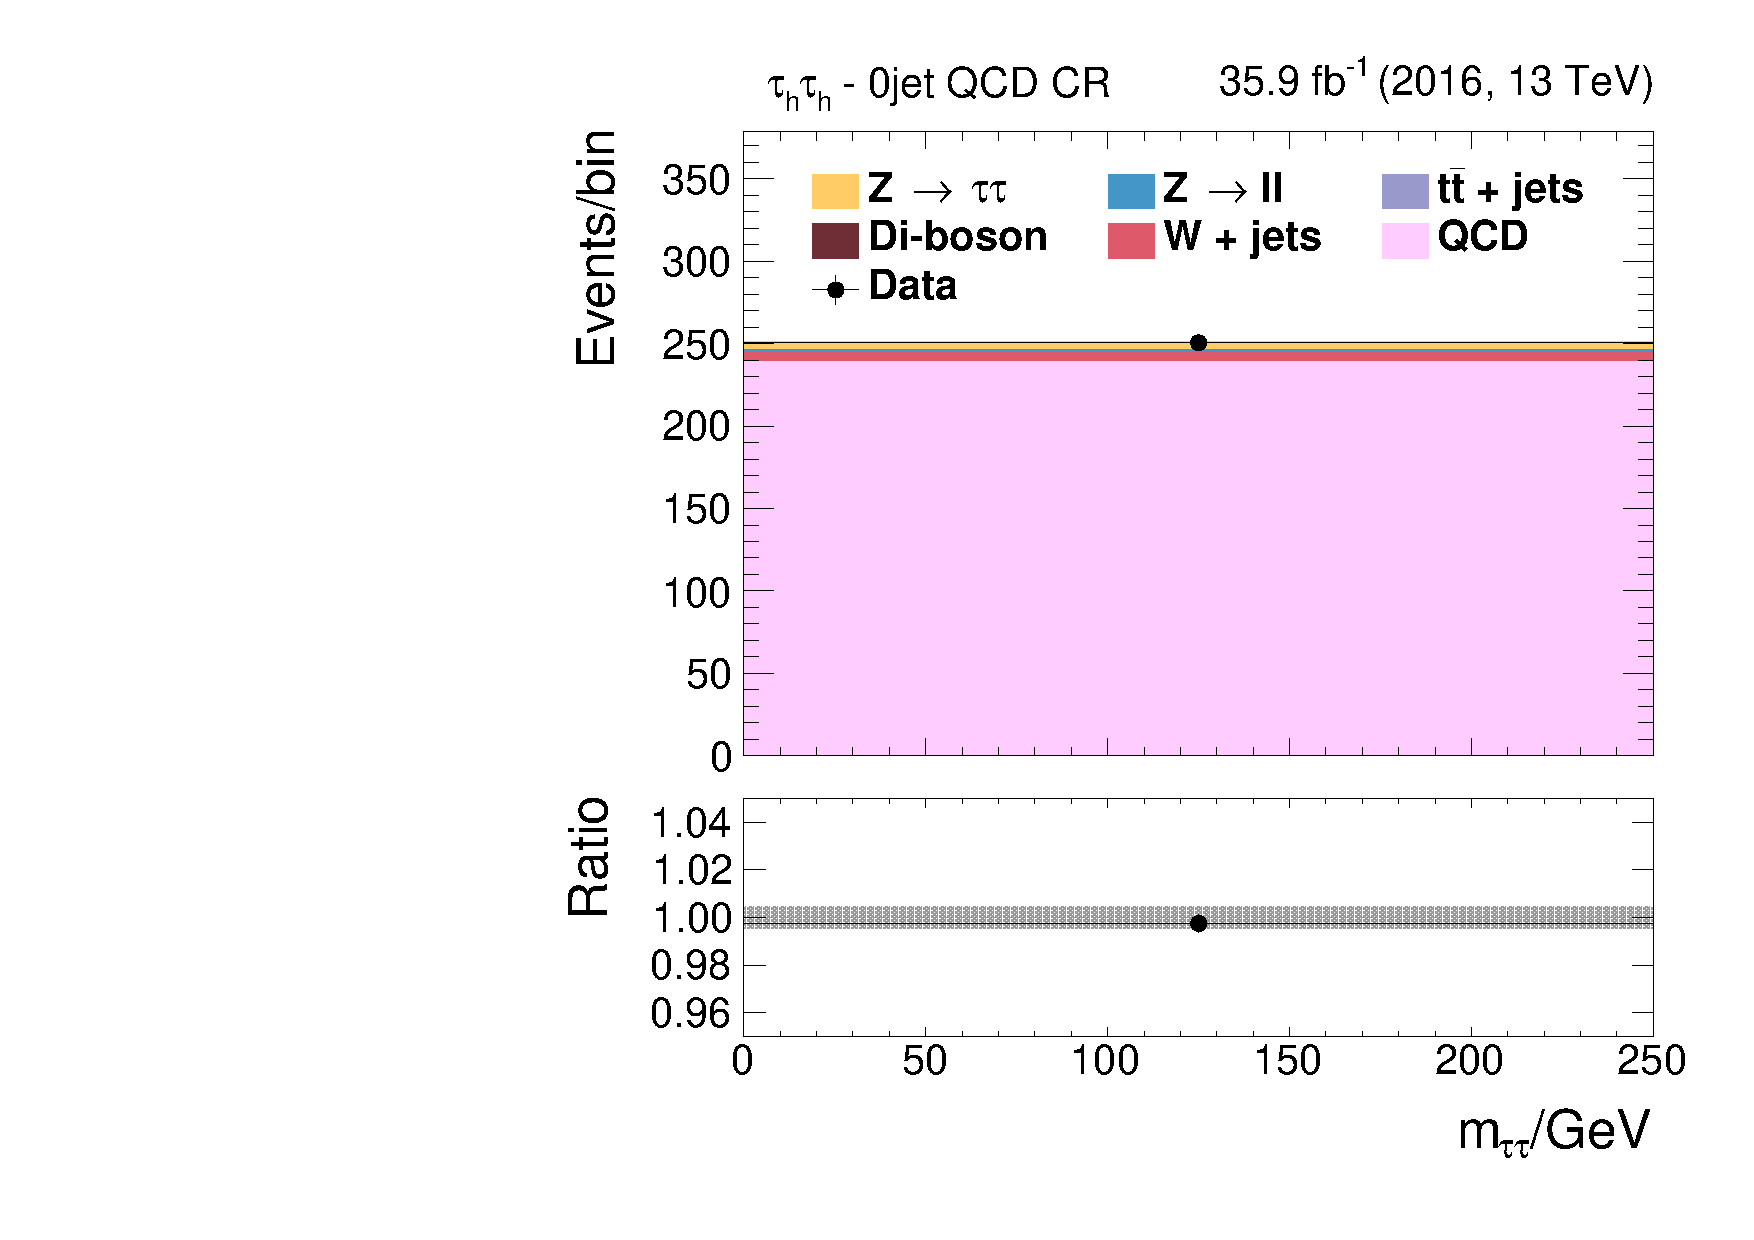
\includegraphics[width=0.47\textwidth]{Figures/background_estimation/qcd_tt_control-regions/htt_inputtt10__htt_tt_10_13TeV.pdf}
    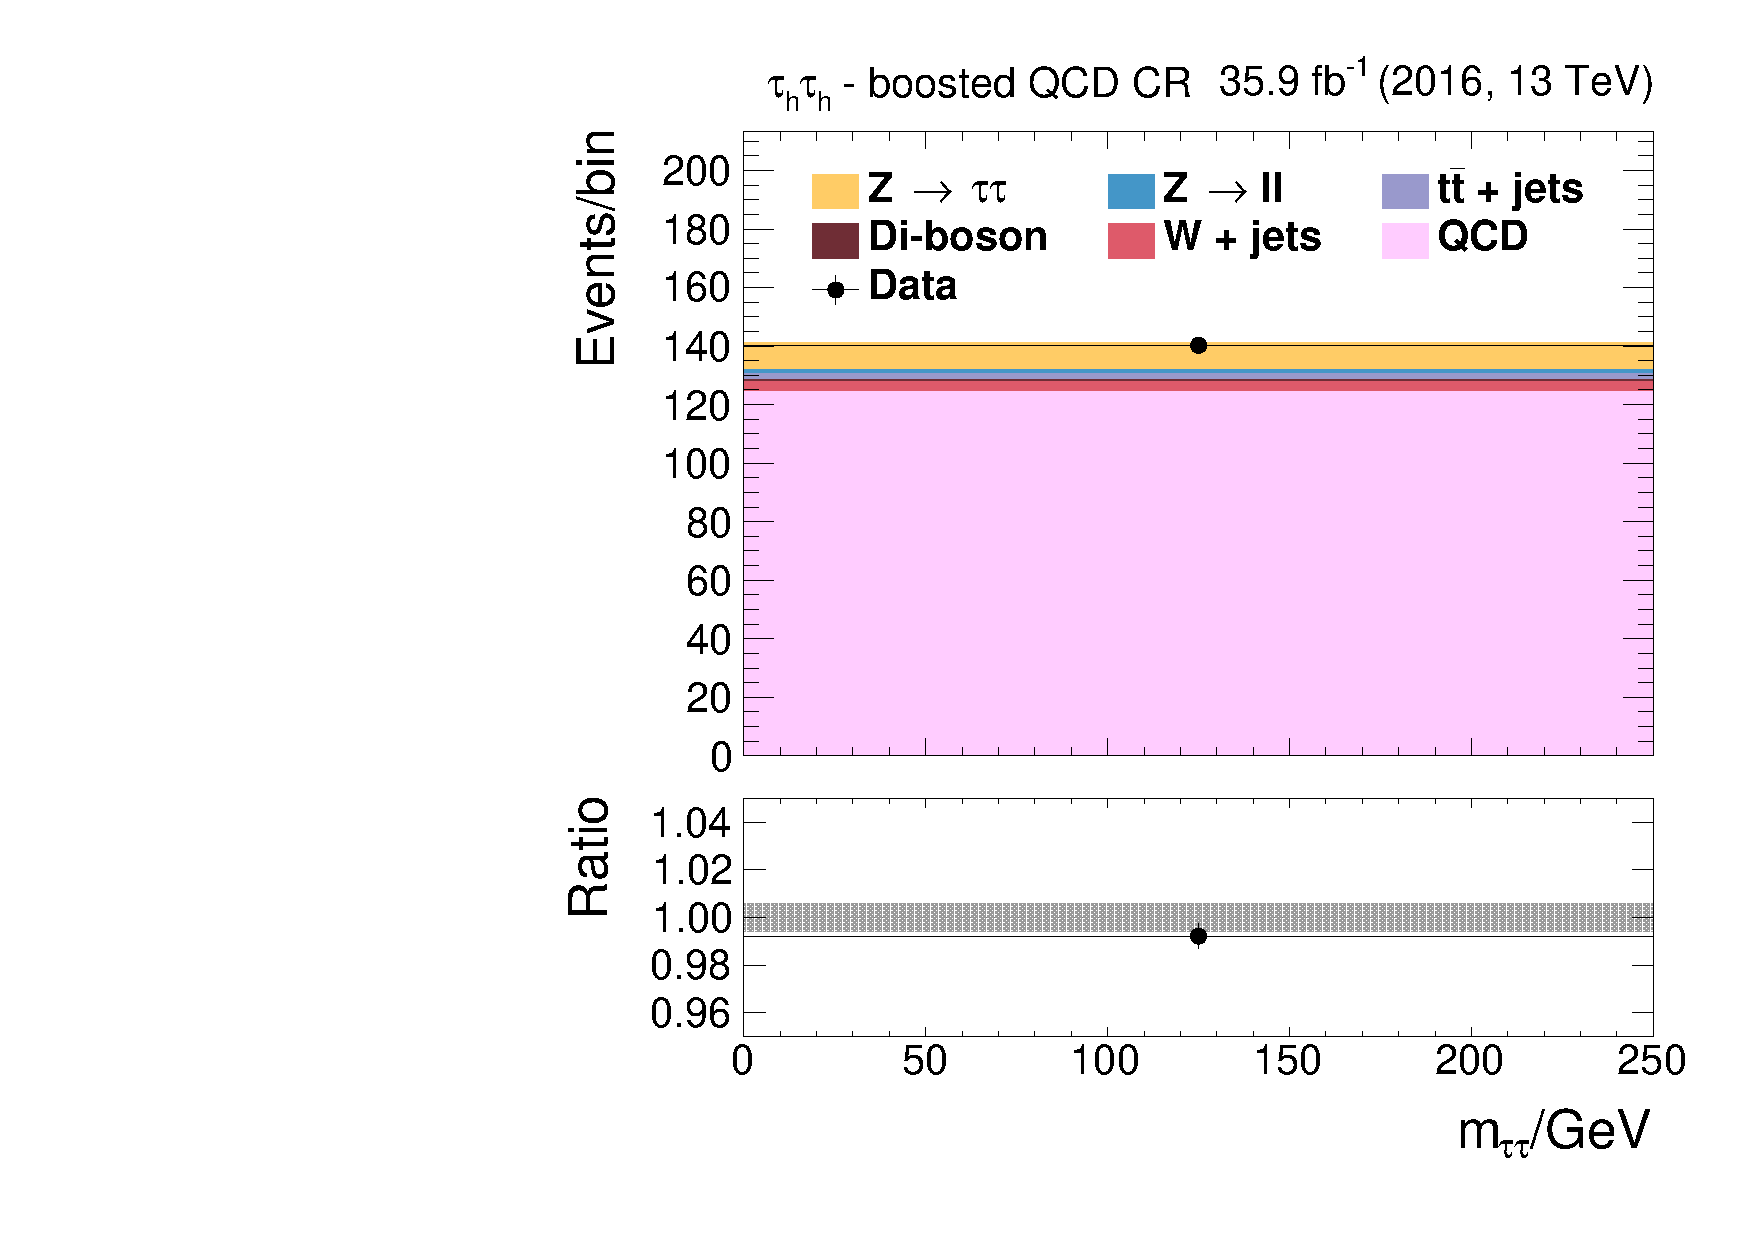
\includegraphics[width=0.47\textwidth]{Figures/background_estimation/qcd_tt_control-regions/htt_inputtt11__htt_tt_11_13TeV.pdf} \\
    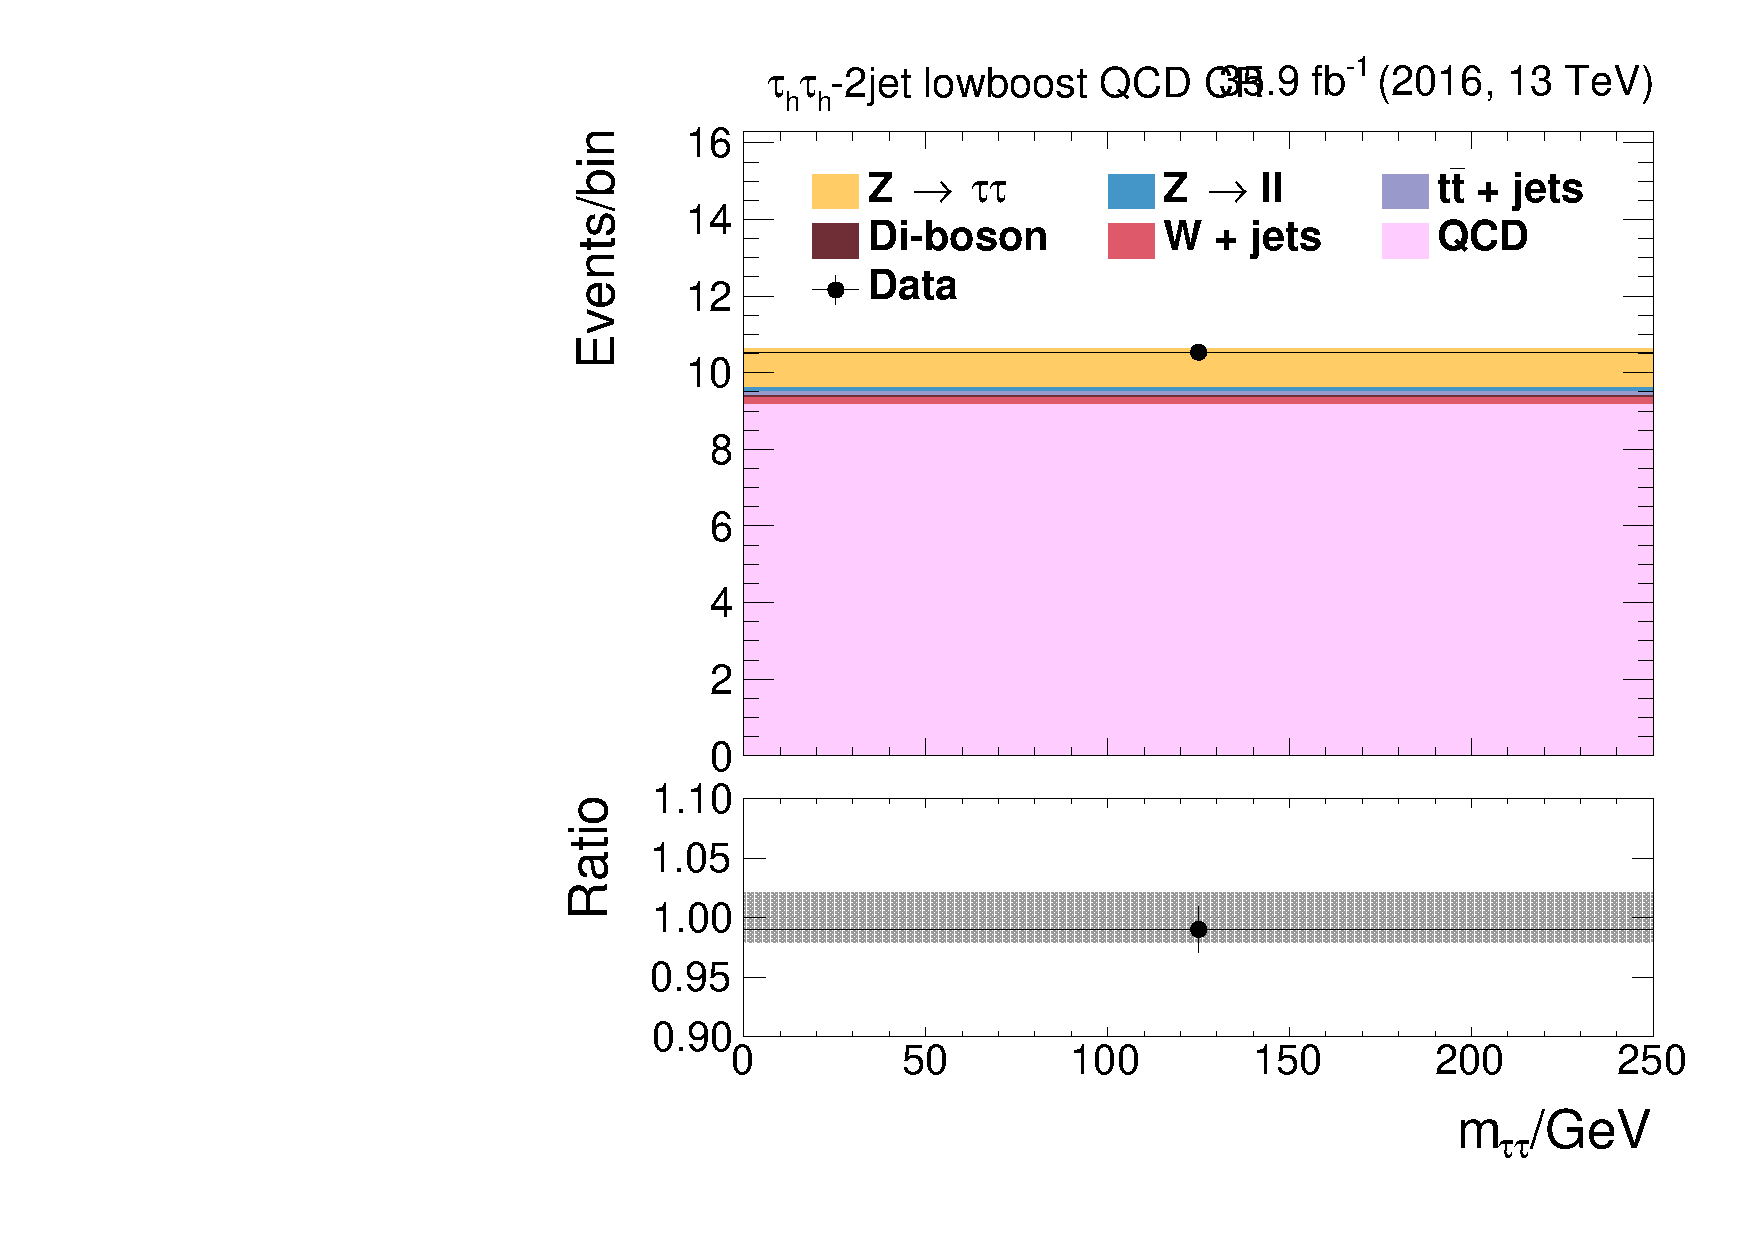
\includegraphics[width=0.47\textwidth]{Figures/background_estimation/qcd_tt_control-regions/htt_inputtt12__htt_tt_12_13TeV.pdf}
    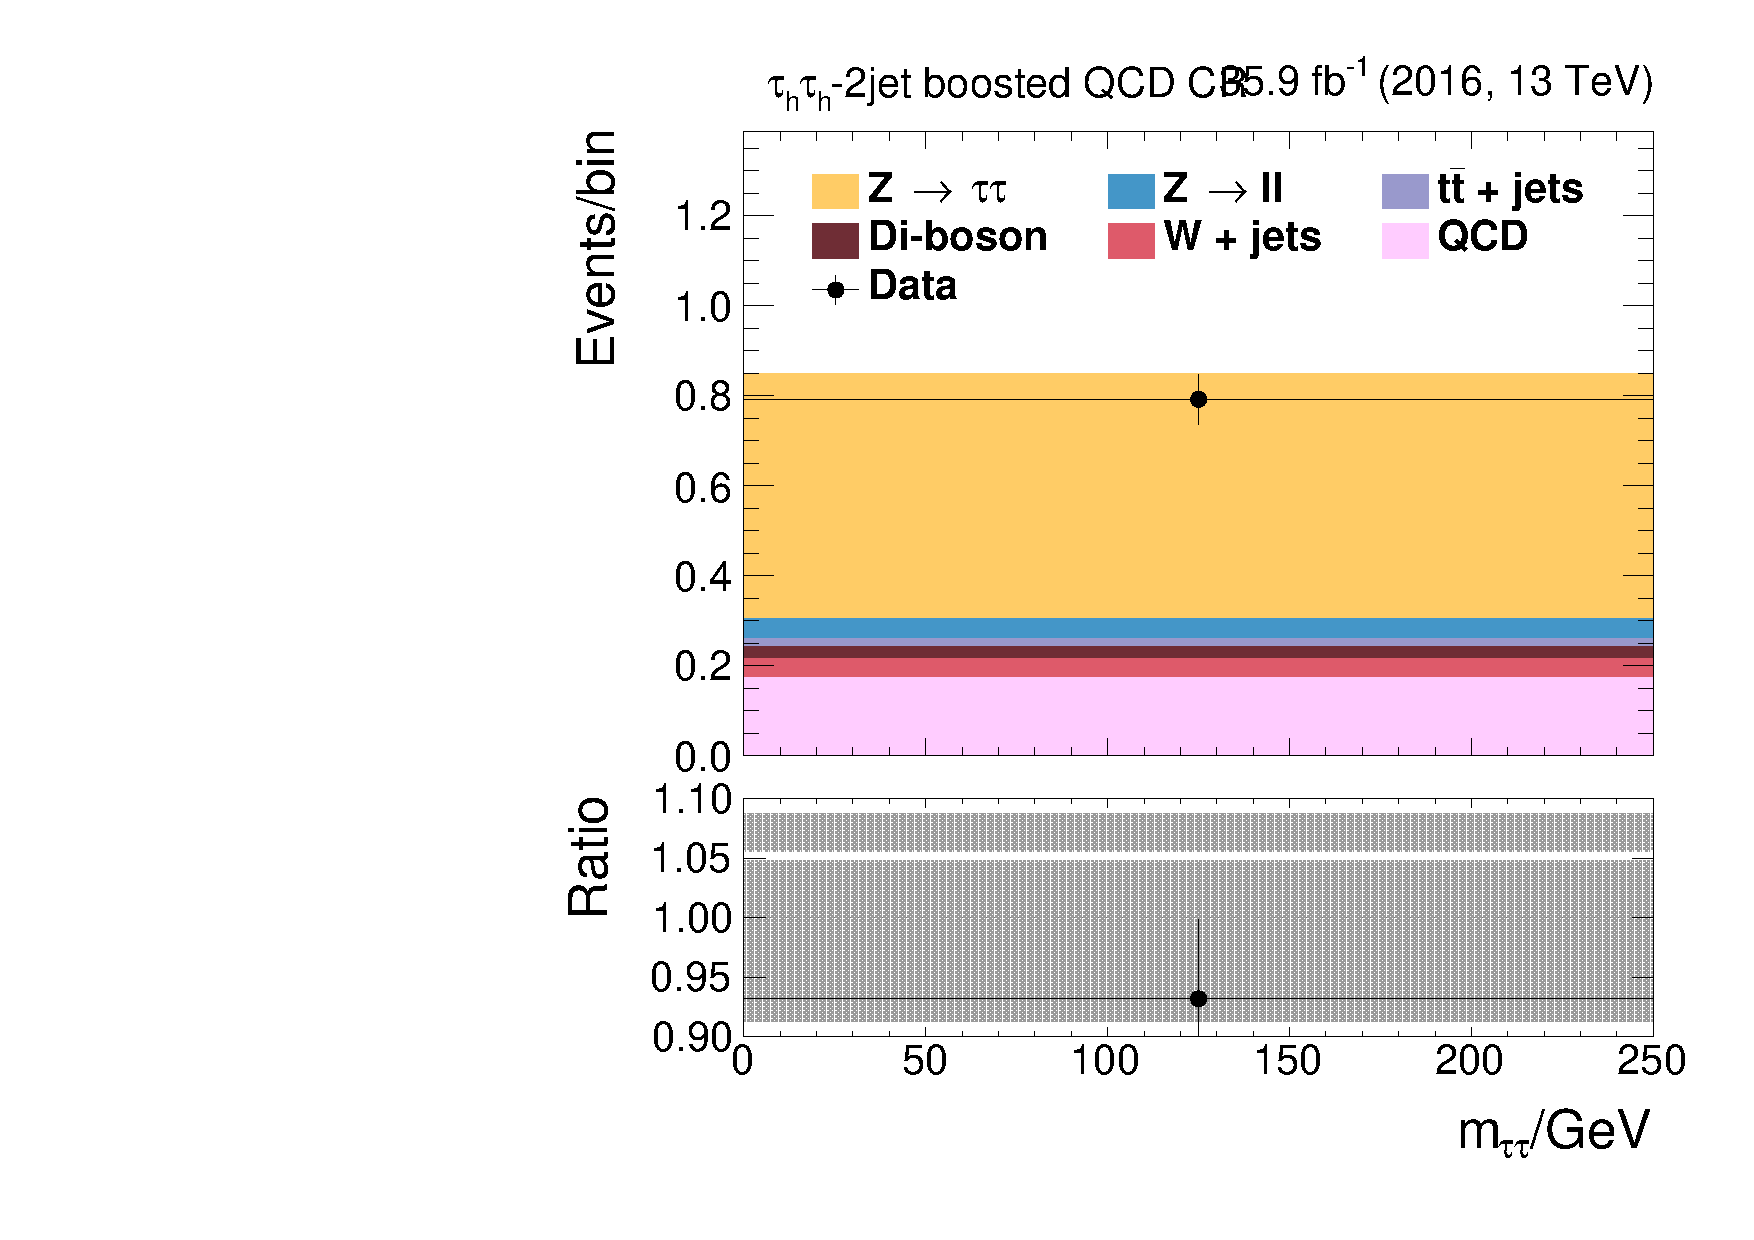
\includegraphics[width=0.47\textwidth]{Figures/background_estimation/qcd_tt_control-regions/htt_inputtt13__htt_tt_13_13TeV.pdf} 
    \caption{Background modeling and data of the QCD control regions in the $\tau_\text{h}\tau_\text{h}$ final state. The \textit{0-jet} (upper left), \textit{boosted} (upper right) and \textit{dijet lowboost} (bottom left) control regions reach purities in the QCD background above 85\%.
    The \textit{dijet boosted} category (bottom right) only a purity of 20\%.}\label{bkg:tt_crs}
\end{figure}

\subsection{VBF Higgs}
Higgs bosons produced via vector boson fusion (VBF) are an important background in this analysis as their two quark-initiated forward jets 
are likely to be misidentified as the signature of the two jets expected for the ggH signal. Dedicated JHU samples are used to derive the shape and yield of this background \tabref{ES:jhu_samples_xsecs}. 
As it must be accounted for the possibility of CP violation also in this vector boson coupling of the Higgs boson, the shape and normalization of the $\mathsf{qq\rightarrow H}$ background is modeled by the physics model introduced in \textreft{SA:physicsmodel}.

\subsection{Other backgrounds}
There are other smaller sources of background such as events with two vector bosons or events with single top quarks
and top-quarks in association with a W boson. The shapes and yields of these backgrounds are fully determined by simulation. 
As for the $\mathsf{Z\rightarrow \tau\tau}$ background they are categorized according to the match of the reconstructed $\tau_\text{h}$ and the generated object. 
This means there are two contributions 
\begin{ct_version_list}
    \item VVT: $\tau_\text{h}$ is matched to the generated hadronic tau in $e\tau_\text{h}$, $\mu\tau_\text{h}$ or $\tau_\text{h}\tau_\text{h}$.
    \item VVJ: otherwise.
\end{ct_version_list}
